% !TEX program = xelatex
% IC Compiler II Timing Analysis User Guide — 中文学习译本
% 原版：Version M-2016.12-SP4, June 2017 (Synopsys)
\documentclass[UTF8,a4paper,openany,oneside]{ctexbook}

% 与 ctexbook + XeLaTeX 配合；中文字体由本文件设置
\usepackage{geometry}
\geometry{a4paper, margin=2.5cm, headheight=14pt}

% Windows 默认；若缺字体请改成本机已安装的中文字体名
\setCJKmainfont{SimSun}
\setCJKsansfont{Microsoft YaHei}
\setCJKmonofont{FangSong}
\setmainfont{Times New Roman}
\setmonofont{Consolas}[Scale=0.92]

\usepackage{graphicx}
\graphicspath{{figures/}}
\usepackage{booktabs}
\usepackage{longtable}
\usepackage{tabularx}
\usepackage{multirow}
\usepackage{array}
\usepackage{enumitem}
\usepackage{xcolor}
\usepackage{fancyhdr}
\usepackage{titlesec}
\usepackage{caption}
\usepackage{listings}
\usepackage{tcolorbox}
\usepackage{amsmath}
\usepackage{microtype}
\usepackage{hyperref}

\hypersetup{
  colorlinks=true,
  linkcolor=blue!50!black,
  urlcolor=blue!60!black,
  citecolor=green!40!black,
  bookmarksnumbered=true,
  pdftitle={IC Compiler II Timing Analysis User Guide 中文学习译本},
  pdfauthor={Unofficial Study Translation}
}

\pagestyle{fancy}
\fancyhf{}
\fancyhead[L]{\small ICC2 Timing Analysis UG M-2016.12-SP4}
\fancyhead[R]{\small 中文学习译本}
\fancyfoot[C]{\thepage}
\renewcommand{\headrulewidth}{0.4pt}

\titleformat{\chapter}[display]
  {\Huge\bfseries}{\chaptertitlename\ \thechapter}{12pt}{\Huge}
\titleformat{\section}{\Large\bfseries}{\thesection}{1em}{}
\titleformat{\subsection}{\large\bfseries}{\thesubsection}{1em}{}
\titleformat{\subsubsection}{\normalsize\bfseries}{\thesubsubsection}{1em}{}

\newcommand{\bichapter}[2]{%
  \chapter[#1]{#1\\[0.35em]{\LARGE\normalfont\itshape #2}}%
}

\tcbuselibrary{skins,breakable}
\newtcolorbox{noteBox}{
  colback=yellow!8, colframe=orange!60!black,
  fonttitle=\bfseries, title=注意,
  breakable, left=4pt, right=4pt
}
\newtcolorbox{seeAlsoBox}{
  colback=blue!4, colframe=blue!50!black,
  fonttitle=\bfseries, title=参见,
  breakable, left=4pt, right=4pt
}

\lstdefinestyle{tcl}{
  language=Tcl,
  basicstyle=\ttfamily\small,
  keywordstyle=\color{blue!70!black}\bfseries,
  commentstyle=\color{green!40!black}\itshape,
  stringstyle=\color{red!60!black},
  showstringspaces=false,
  breaklines=true,
  frame=single,
  rulecolor=\color{black!30},
  backgroundcolor=\color{gray!5},
  columns=fullflexible,
  keepspaces=true,
  tabsize=2,
  captionpos=b,
  literate={–}{{-}}1
}
\lstset{style=tcl}
\newcommand{\cmd}[1]{\texttt{#1}}
\newcommand{\opt}[1]{\texttt{#1}}
\newcommand{\appopt}[1]{\texttt{#1}}

\captionsetup{font=small, labelfont=bf}
\renewcommand{\figurename}{图}
\renewcommand{\tablename}{表}
\renewcommand{\lstlistingname}{代码}

\setlist[itemize]{leftmargin=1.8em, itemsep=0.25em, topsep=0.4em}
\setlist[enumerate]{leftmargin=1.8em, itemsep=0.25em, topsep=0.4em}

\newcommand{\copyrightnotice}{%
\begin{center}
\small
原文版权归 Synopsys, Inc.\ 所有（Version M-2016.12-SP4, June 2017）。\\
本文件为\textbf{非官方个人学习译本}，仅供学习参考，不得用于商业传播。\\
命令名、选项名、文件名等技术标识符保持英文原文不译。\\
插图截自原版 PDF，图中英文标注保留。
\end{center}
}


\begin{document}

% -------------------- 封面 --------------------
\begin{titlepage}
  \centering
  \vspace*{2cm}
  {\Huge\bfseries IC Compiler\texttrademark\ II}\\[0.6em]
  {\Huge\bfseries Timing Analysis User Guide}\\[1.2em]
  {\LARGE 中文学习译本}\\[2em]
  {\large 原版版本：M-2016.12-SP4，June 2017}\\[0.5em]
  {\large Synopsys, Inc.}\\[3em]
  \begin{minipage}{0.85\textwidth}
    \copyrightnotice
  \end{minipage}
  \vfill
  {\large 基于官方 PDF 的结构化翻译}\\[0.3em]
  {\normalsize 前言 + 第~1--7~章}
\end{titlepage}

\frontmatter
\tableofcontents
\clearpage
% 前言 Preface
\chapter*{关于本用户指南}
\addcontentsline{toc}{chapter}{关于本用户指南}
\chaptermark{关于本用户指南}

\noindent\textit{About This User Guide}

Synopsys IC Compiler II 工具提供从网表到 GDSII 的完整设计方案，在整个设计流程中结合专有的设计规划、物理综合、时钟树综合与布线，完成逻辑与物理实现。

本指南说明 IC Compiler II 的实现与集成流程。有关该工具的更多信息，请参阅下列配套文档：
\begin{itemize}
  \item \textit{IC Compiler II Library Preparation User Guide}
  \item \textit{IC Compiler II Design Planning User Guide}
  \item \textit{IC Compiler II Data Model User Guide}
  \item \textit{IC Compiler II Implementation User Guide}
  \item \textit{IC Compiler II Graphical User Interface User Guide}
\end{itemize}

\section*{读者对象}
\addcontentsline{toc}{section}{读者对象}

本用户指南面向使用 IC Compiler II 实现设计的设计工程师。

使用该工具需要具备物理设计与综合技能，并熟悉以下内容：
\begin{itemize}
  \item 物理设计原理
  \item Linux 或 UNIX 操作系统
  \item 工具命令语言（Tcl）
\end{itemize}

\section*{相关出版物}
\addcontentsline{toc}{section}{相关出版物}

有关 IC Compiler II 的更多信息，请参阅 Synopsys SolvNet 在线支持站点上的文档：
\url{https://solvnet.synopsys.com/DocsOnWeb}

您可能还希望参阅以下相关 Synopsys 产品文档：
\begin{itemize}
  \item Design Compiler\textsuperscript{\textregistered}
  \item IC Validator
  \item PrimeTime\textsuperscript{\textregistered} Suite
\end{itemize}

\section*{发行说明}
\addcontentsline{toc}{section}{发行说明}

关于新功能、增强与变更、已知限制，以及已解决的 Synopsys Technical Action Requests（STAR）信息，请参阅 SolvNet 站点上的 \textit{IC Compiler II Release Notes}。

查看发行说明的步骤：
\begin{enumerate}
  \item 打开 SolvNet Download Center：\url{https://solvnet.synopsys.com/DownloadCenter}
  \item 选择 IC Compiler II，再在出现的列表中选择一个发行版本。
\end{enumerate}

\section*{排版约定}
\addcontentsline{toc}{section}{排版约定}

Synopsys 文档使用下列约定。

\begin{table}[htbp]
\centering
\caption{文档排版约定}
\begin{tabularx}{\textwidth}{@{}>{\bfseries}l X@{}}
\toprule
约定 & 说明 \\
\midrule
Courier & 表示语法，例如 \cmd{write\_file} \\
Courier italic & 表示语法中的用户自定义值，例如 \cmd{write\_file design\_list} \\
Courier bold & 表示示例中用户原样输入的内容，例如 \texttt{prompt> write\_file top} \\
\cmd{[]} & 表示语法中的可选参数，例如 \cmd{write\_file [-format fmt]} \\
\cmd{...} & 表示参数可按需重复，例如 \cmd{pin1 pin2 ... pinN} \\
\cmd{|} & 表示在多个备选中选择其一，例如 \cmd{low | medium | high} \\
Ctrl+C & 表示组合键，例如按住 Ctrl 再按 C \\
\cmd{\textbackslash} & 表示命令行续行 \\
\cmd{/} & 表示目录层次 \\
Edit $>$ Copy & 表示菜单命令路径，例如打开 Edit 菜单并选择 Copy \\
\bottomrule
\end{tabularx}
\end{table}

\section*{客户支持}
\addcontentsline{toc}{section}{客户支持}

客户支持通过 SolvNet 在线客户支持以及 Synopsys 技术支持中心提供。

\subsection*{访问 SolvNet}

SolvNet 站点包含技术文章知识库以及对 Synopsys 工具常见问题的解答，并可访问软件下载、文档与技术支持等在线服务。

访问地址：\url{https://solvnet.synopsys.com}

如提示，请输入用户名与密码。若尚无 Synopsys 账号，请按页面说明注册。
若使用 SolvNet 时需要帮助，请点击右上角菜单栏中的 \textbf{HELP}。

\subsection*{联系 Synopsys 技术支持中心}

若有问题、疑问或建议，可通过以下方式联系 Synopsys Technical Support Center：
\begin{itemize}
  \item 登录 SolvNet（\url{https://solvnet.synopsys.com}），点击 Support，再点击 ``Open A Support Case''，向本地支持中心提交支持案例。
  \item 向本地支持中心发送电子邮件。
  \begin{itemize}
    \item 北美地区：\texttt{support\_center@synopsys.com}
    \item 其他地区地址见 \url{http://www.synopsys.com/Support/GlobalSupportCenters/Pages}
  \end{itemize}
  \item 致电本地支持中心。
  \begin{itemize}
    \item 北美地区：(800) 245-8005
    \item 其他地区电话见 \url{http://www.synopsys.com/Support/GlobalSupportCenters/Pages}
  \end{itemize}
\end{itemize}


\mainmatter
% 第 1 章 Defining Modes, Corners, and Scenarios
\bichapter{定义模式、corner 与 scenario}{Defining Modes, Corners, and Scenarios}
\label{chap:mcs}

一个 block 可能在多种条件下工作，例如不同的温度与电压，也可能处于多种功能模式。做时序分析时，每一组条件用一个 corner 表示，每一种功能模式用一个 mode 表示。scenario 是 corner 与 mode 的组合，用于时序分析与优化。

开始处理 block 之前，必须定义该 block 使用的 mode、corner 与 scenario，并定义与之关联的约束。本章包括以下主题：
\begin{itemize}
  \item 创建与删除 mode
  \item 查询 mode
  \item 创建与删除 corner
  \item 查询 corner
  \item 创建 scenario
  \item 设置 scenario 的有效分析类型
  \item 查询 scenario
  \item 删除重复的 scenario、mode 与 corner
  \item IC Compiler II 时序约束
  \item 设置时序约束
  \item 为 IC Compiler II 时序分析转换 SDC 文件
  \item 从 Design Compiler 或 IC Compiler 导入时序约束
  \item 删除 SDC 约束
\end{itemize}

\section{创建与删除 mode}
\subsection*{Creating and Removing Modes}

用 \cmd{create\_mode} 创建功能模式。每个 mode 的名称必须唯一。

例如，创建名为 \cmd{mode1} 的 mode：
\begin{lstlisting}
icc2_shell> create_mode mode1
\end{lstlisting}

用 \cmd{current\_mode} 把当前 mode 切换到指定 mode：
\begin{lstlisting}
icc2_shell> current_mode mode1
\end{lstlisting}

用 \cmd{remove\_modes} 删除当前 block 的 mode。\opt{-all} 删除全部 mode；也可使用 Tcl 列表或 collection 指定要删除的 mode。删除某个 mode 时，与该 mode 关联的全部 scenario 一并删除。

例如，删除 \cmd{mode1} 与 \cmd{mode2}：
\begin{lstlisting}
icc2_shell> remove_modes {mode1 mode2}
\end{lstlisting}

\section{查询 mode}
\subsection*{Querying Modes}

可获取以下信息：
\begin{itemize}
  \item 当前 mode：不带参数调用 \cmd{current\_mode}。
\begin{lstlisting}
icc2_shell> current_mode
{"mode1"}
\end{lstlisting}
  \item block 上已定义的 mode 列表：使用 \cmd{get\_modes}。\\
        默认返回包含当前 block 全部 mode 的 collection（与 \cmd{all\_modes} 类似）。要取得其他 block 的 mode，使用 \opt{-design}。\\
        可按属性值（\opt{-filter}）、关联的 corner（\opt{-of\_objects}）或名称模式过滤返回的 mode。
  \item 当前 block 一个或多个 mode 的详细信息：使用 \cmd{report\_modes}。\\
        报告包含每个 mode 关联的 scenario 及其有效分析类型。
\end{itemize}

报告当前 block 全部 mode 的详细信息：
\begin{lstlisting}
icc2_shell> report_modes
\end{lstlisting}

报告名为 \cmd{mode1} 与 \cmd{mode2} 的 mode：
\begin{lstlisting}
icc2_shell> report_modes {mode1 mode2}
\end{lstlisting}

\begin{seeAlsoBox}
设置 scenario 的有效分析类型
\end{seeAlsoBox}

\section{创建与删除 corner}
\subsection*{Creating and Removing Corners}

用 \cmd{create\_corner} 创建时序 corner。每个 corner 的名称必须唯一。

例如，创建名为 \cmd{corner1} 的 corner：
\begin{lstlisting}
icc2_shell> create_corner corner1
\end{lstlisting}

用 \cmd{current\_corner} 切换当前 corner：
\begin{lstlisting}
icc2_shell> current_corner corner1
\end{lstlisting}

用 \cmd{remove\_corners} 删除当前 block 的 corner。\opt{-all} 删除全部 corner；也可使用 Tcl 列表或 collection 指定 corner。删除某个 corner 时，与该 corner 关联的全部 scenario 一并删除。

例如，删除 \cmd{corner1} 与 \cmd{corner2}：
\begin{lstlisting}
icc2_shell> remove_corners {corner1 corner2}
\end{lstlisting}

\section{查询 corner}
\subsection*{Querying Corners}

可获取以下信息：
\begin{itemize}
  \item 当前 corner：不带参数调用 \cmd{current\_corner}。
\begin{lstlisting}
icc2_shell> current_corner
{"corner1"}
\end{lstlisting}
  \item block 上已定义的 corner 列表：使用 \cmd{get\_corners}。\\
        默认返回包含当前 block 全部 corner 的 collection（与 \cmd{all\_corners} 类似）。其他 block 使用 \opt{-design}。\\
        可按属性值（\opt{-filter}）、关联对象（\opt{-of\_objects}）或名称模式过滤。
  \item 当前 block 一个或多个 corner 的详细信息：使用 \cmd{report\_corners}。\\
        报告包含每个 corner 关联的 scenario 及其有效分析类型。
\end{itemize}

报告当前 block 全部 corner：
\begin{lstlisting}
icc2_shell> report_corners
\end{lstlisting}

报告名为 \cmd{corner1} 与 \cmd{corner2} 的 corner：
\begin{lstlisting}
icc2_shell> report_corners {corner1 corner2}
\end{lstlisting}

\section{创建 scenario}
\subsection*{Creating a Scenario}

用 \cmd{create\_scenario} 创建时序 scenario。每个 scenario 的名称必须唯一。默认情况下，新建 scenario 组合当前 mode 与当前 corner。用 \opt{-mode} 指定 mode，用 \opt{-corner} 指定 corner。

例如，创建名为 \cmd{scenario1} 的 scenario，组合 \cmd{mode1} 与 \cmd{corner1}：
\begin{lstlisting}
icc2_shell> create_scenario -mode mode1 -corner corner1 -name scenario1
\end{lstlisting}

创建 scenario 时，默认它处于 active 状态、对全部分析类型启用，并成为当前 scenario。同时，它的 mode 成为当前 mode，它的 corner 成为当前 corner。

用 \cmd{set\_scenario\_status -active true|false} 改变 scenario 的 active 状态。用 \cmd{set\_scenario\_status} 修改其有效分析类型。

用 \cmd{remove\_scenarios} 删除当前 block 的 scenario。\opt{-all} 删除全部 scenario；也可使用 Tcl 列表或 collection 指定要删除的 scenario。

例如，删除 \cmd{scenario1} 与 \cmd{scenario2}：
\begin{lstlisting}
icc2_shell> remove_scenarios {scenario1 scenario2}
\end{lstlisting}

\begin{seeAlsoBox}
设置 scenario 的有效分析类型
\end{seeAlsoBox}

\section{设置 scenario 的有效分析类型}
\subsection*{Setting the Active Analysis Types for a Scenario}

默认情况下，scenario 处于 active 状态，并对全部分析类型启用。用 \cmd{set\_scenario\_status} 修改一个或多个 scenario 的有效分析类型，选项见表~\ref{tab:scenario-status}。

可用 \opt{-active false} 临时关闭各项分析设置。使用该选项时，指定 scenario 的全部分析被禁用，但各项设置仍保留在设计库中。再用 \opt{-active true} 时，各项设置重新生效。

\begin{table}[htbp]
\centering
\caption{\cmd{set\_scenario\_status} 的分析选项}
\label{tab:scenario-status}
\begin{tabular}{@{}ll@{}}
\toprule
分析类型 & 命令选项 \\
\midrule
全部 & \cmd{-all} \\
无 & \cmd{-none} \\
建立时间（setup） & \cmd{-setup true | false} \\
保持时间（hold） & \cmd{-hold true | false} \\
泄漏功耗 & \cmd{-leakage\_power true | false} \\
动态功耗 & \cmd{-dynamic\_power true | false} \\
最大转换时间 & \cmd{-max\_transition true | false} \\
最大电容 & \cmd{-max\_capacitance true | false} \\
最小电容 & \cmd{-min\_capacitance true | false} \\
\bottomrule
\end{tabular}
\end{table}

\section{查询 scenario}
\subsection*{Querying Scenarios}

可获取以下信息：
\begin{itemize}
  \item 当前 scenario：不带参数调用 \cmd{current\_scenario}。
\begin{lstlisting}
icc2_shell> current_scenario
{"scenario1"}
\end{lstlisting}
  \item block 上已定义的 scenario：使用 \cmd{get\_scenarios}。\\
        默认返回包含当前 block 全部 scenario 的 collection（与 \cmd{all\_scenarios} 类似）。\\
        可按属性值（\opt{-filter}）、关联 corner（\opt{-corners}）、关联 mode（\opt{-modes}）或名称模式过滤。
  \item 当前 block 一个或多个 scenario 的详细信息：使用 \cmd{report\_scenarios}。\\
        报告包含每个 scenario 的名称、关联 mode、关联 corner 以及有效分析类型。\\
        默认报告当前 block 的全部 scenario。还可以：
  \begin{itemize}
    \item 用 \opt{-scenarios} 报告指定 scenario；
    \item 用 \opt{-modes} 报告与指定 mode 关联的 scenario；
    \item 用 \opt{-corners} 报告与指定 corner 关联的 scenario。
  \end{itemize}
\end{itemize}

报告当前 block 全部 scenario：
\begin{lstlisting}
icc2_shell> report_scenarios
\end{lstlisting}

报告名为 \cmd{scenario1} 与 \cmd{scenario2} 的 scenario：
\begin{lstlisting}
icc2_shell> report_scenarios -scenarios {scenario1 scenario2}
\end{lstlisting}

\section{删除重复的 scenario、mode 与 corner}
\subsection*{Removing Duplicate Scenarios, Modes, and Corners}

为改善运行时间与容量，可用 \cmd{remove\_duplicate\_timing\_contexts} 删除重复的 scenario、corner 与 mode。该命令会：
\begin{itemize}
  \item 删除重复且 scenario 状态相同的 scenario。
  \item 把重复 mode 上的 scenario 重新归到一个公共 mode，并删除重复 mode。重新分配 scenario 时，必要时会创建新的 corner。
  \item 把重复 corner 上的 scenario 重新归到一个公共 corner，并删除重复 corner。
\end{itemize}

判断重复 mode 时，工具不考虑已反标的开关活动（switching activity）。因此运行该命令后需要重新施加开关活动。

若使用 \cmd{set\_block\_to\_top\_map} 把 block 级的 mode、corner 与 scenario 映射到顶层，运行 \cmd{remove\_duplicate\_timing\_contexts} 之后必须手工更新该映射。用 \cmd{report\_block\_to\_top\_map} 查看顶层与 block 级 mode、corner、scenario 之间的关系。

\section{IC Compiler II 时序约束}
\subsection*{IC Compiler II Timing Constraints}

IC Compiler II 把时序约束分为以下几类：
\begin{itemize}
  \item \textbf{Mode 专用约束}\\
        定义或修改时序图（timing graph，表示电路时序的加权图）的约束是 mode 专用约束，包括：
  \begin{itemize}
    \item 时钟定义
    \item 最大与最小延迟约束
  \end{itemize}
        至少应为每个时钟信号包含一条时钟定义。
  \item \textbf{Corner 专用约束}\\
        修改对象上计算延迟的约束是 corner 专用约束，包括：
  \begin{itemize}
    \item 工作条件（operating conditions）
    \item 端口负载电容
    \item 寄生参数信息与缩放因子
    \item 时序 derating 因子
  \end{itemize}
  \item \textbf{Scenario 专用约束}\\
        带有延迟值并引用 modal 对象（例如时钟）的约束是 scenario 专用约束，包括：
  \begin{itemize}
    \item 输入与输出延迟
    \item 时钟特性，例如 clock latency、uncertainty 与 transition
  \end{itemize}
        至少应为每个 I/O 端口包含输入延迟或输出延迟。
  \item \textbf{网表专用约束}\\
        适用于全部 corner、mode 与 scenario 的约束是网表专用约束，包括 ideal network 设置。\\
        它们可以全局作用于全部设计，也可以局部作用于某个设计。例如 \cmd{set\_ideal\_network} 设置的约束就是网表专用的。
\end{itemize}

\section{设置时序约束}
\subsection*{Setting Timing Constraints}

可以通过读入 Synopsys Design Constraints（SDC）文件，或逐条执行 SDC 命令来指定时序约束。SDC 命令的细节见 \textit{Using the Synopsys Design Constraints Format Application Note}。

用 \cmd{read\_sdc} 读入 SDC 文件：
\begin{lstlisting}
icc2_shell> read_sdc block.sdc
\end{lstlisting}

\begin{noteBox}
若 SDC 文件不含单位设置，单位取自主逻辑库。若 SDC 文件含有单位设置，则必须与主逻辑库中的单位一致。
\end{noteBox}

为使 block 设置高效且准确，按以下步骤操作：
\begin{enumerate}
  \item 把 block 约束拆成下列独立文件：
  \begin{itemize}
    \item 每个 mode 一个 mode 专用文件
    \item 每个 corner 一个 corner 专用文件
    \item 每个 scenario 一个 scenario 专用文件
    \item block 的全局约束文件
  \end{itemize}
  \item 为该 block 定义全部 mode、corner 与 scenario。
  \item 在施加对应约束之前，先把当前 mode、corner 或 scenario 设对。\\
        读入 SDC 文件或执行 SDC 命令时，约束按类型只作用于当前 scenario，或其关联的 mode / corner。
\end{enumerate}

例如，假设某 block 具有：
\begin{itemize}
  \item 两个 mode：\cmd{M1} 与 \cmd{M2}
  \item 一个 corner：\cmd{C}
  \item 两个 scenario：
  \begin{itemize}
    \item \cmd{M1@C}，由 mode \cmd{M1} 与 corner \cmd{C} 组合
    \item \cmd{M2@C}，由 mode \cmd{M2} 与 corner \cmd{C} 组合
  \end{itemize}
\end{itemize}

下列脚本创建 mode、corner 与 scenario，并施加对应约束与设置：
\begin{lstlisting}
# Create all modes, corners, and scenarios
create_mode M1
create_mode M2
create_corner C
create_scenario -mode M1 -corner C -name M1@C
create_scenario -mode M2 -corner C -name M2@C
# Apply mode-, corner-, and scenario-specific constraints
current_mode M1
read_sdc M1_mode.sdc
current_mode M2
read_sdc M2_mode.sdc
current_corner C
read_sdc C_corner.sdc
## Apply TLUPlus settings, extraction options, and other settings
current_scenario M1@C
read_sdc M1@C_scenario.sdc
current_scenario M2@C
read_sdc M2@C_scenario.sdc
\end{lstlisting}

\section{为 IC Compiler II 时序分析转换 SDC 文件}
\subsection*{Converting an SDC File for IC Compiler II Timing Analysis}

IC Compiler II 只支持 OCV 时序分析。若 SDC 按 best-case/worst-case（BCWC）时序分析编写，必须把它转换成两份 OCV SDC 文件。

把 BCWC SDC 转换成两份 OCV SDC 的步骤：
\begin{enumerate}
  \item 用 \cmd{create\_mode} 为设计创建一个 mode，见「创建与删除 mode」。
\begin{lstlisting}
icc2_shell> create_mode my_mode
\end{lstlisting}
  \item 为 best-case 约束创建：
  \begin{itemize}
    \item 用 \cmd{create\_corner} 创建一个 corner；
    \item 用 \cmd{create\_scenario} 创建一个 scenario。
  \end{itemize}
        best-case scenario 不用于 setup 分析，因此用 \cmd{set\_scenario\_status -setup false} 关闭该 scenario 的 setup 分析。
\begin{lstlisting}
icc2_shell> create_corner bc_corner
icc2_shell> create_scenario -mode my_mode -corner bc_corner \
    -name bc_scenario
icc2_shell> set_scenario_status -setup false bc_scenario
\end{lstlisting}
  \item 用 \cmd{read\_sdc} 从 BCWC SDC 文件读入 best-case 约束。\\
        默认情况下，工具读入 SDC 文件中的全部约束。若只保留 best-case 约束，读入前把应用选项 \appopt{time.convert\_constraint\_from\_bc\_wc} 设为 \cmd{bc\_only}。
\begin{lstlisting}
icc2_shell> set_app_options \
    -name time.convert_constraint_from_bc_wc -value bc_only
icc2_shell> read_sdc bc_wc.sdc
\end{lstlisting}
  \item 为 worst-case 约束创建 corner 与 scenario。\\
        worst-case scenario 不用于 hold 分析，因此用 \cmd{set\_scenario\_status -hold false} 关闭 hold 分析。
\begin{lstlisting}
icc2_shell> create_corner wc_corner
icc2_shell> create_scenario -mode my_mode -corner wc_corner \
    -name wc_scenario
icc2_shell> set_scenario_status -hold false wc_scenario
\end{lstlisting}
  \item 用 \cmd{read\_sdc} 从同一 BCWC SDC 文件读入 worst-case 约束。\\
        读入前把 \appopt{time.convert\_constraint\_from\_bc\_wc} 设为 \cmd{wc\_only}。
\begin{lstlisting}
icc2_shell> set_app_options \
    -name time.convert_constraint_from_bc_wc -value wc_only
icc2_shell> read_sdc bc_wc.sdc
\end{lstlisting}
  \item 把 \appopt{time.convert\_constraint\_from\_bc\_wc} 复位为 \cmd{none}。
\begin{lstlisting}
icc2_shell> set_app_options \
    -name time.convert_constraint_from_bc_wc -value none
\end{lstlisting}
\end{enumerate}

\section{从 Design Compiler 或 IC Compiler 导入时序约束}
\subsection*{Importing Timing Constraints From the Design Compiler or IC Compiler Tool}

把 Design Compiler 或 IC Compiler 的时序约束导入 IC Compiler II：
\begin{enumerate}
  \item 在 Design Compiler 或 IC Compiler 中用 \cmd{write\_timing\_context -format icc2} 生成约束。\\
        必须用 \opt{-output} 指定输出名称。输出是一个目录，其中包含表~\ref{tab:timing-context} 所列 Tcl 脚本。
\end{enumerate}

\begin{table}[htbp]
\centering
\caption{\cmd{write\_timing\_context -format icc2} 生成的 Tcl 脚本}
\label{tab:timing-context}
\begin{tabularx}{\textwidth}{@{}l X@{}}
\toprule
脚本名 & 内容 \\
\midrule
\cmd{top.tcl} &
创建 mode、corner 与 scenario 的命令；以及向 mode、corner、scenario 和设计填入约束的命令 \\
\cmd{scenario\_<scenario\_name>.tcl} & 特定 scenario 的约束 \\
\cmd{design.tcl} & 与 scenario 无关的设计约束 \\
\bottomrule
\end{tabularx}
\end{table}

默认情况下，该命令为全部 scenario（active 与 inactive）以及 block 上与 scenario 无关的时序约束生成文件。若只生成指定 scenario 的约束，使用 \opt{-scenarios}。

\begin{enumerate}
  \setcounter{enumi}{1}
  \item 在 IC Compiler II 中 source \cmd{top.tcl}，从而创建对应的 mode、corner 与 scenario 并施加约束。
\end{enumerate}

下列示例在 Design Compiler 中为全部 active scenario 以及与 scenario 无关的时序约束生成文件：
\begin{lstlisting}
dc_shell> write_timing_context -scenarios [get_scenarios -active true] \
    -output BLK1_const
\end{lstlisting}

下列示例把 Design Compiler 生成的约束导入 IC Compiler II：
\begin{lstlisting}
icc2_shell> open_block BLK1
icc2_shell> source BLK1_const/top.tcl
\end{lstlisting}

\section{删除 SDC 约束}
\subsection*{Removing SDC Constraints}

用 \cmd{remove\_sdc} 从 block 中删除 SDC 约束。

默认删除当前 block 中的全部 SDC 约束。也可以这样控制删除范围：
\begin{itemize}
  \item 用 \opt{-modes}、\opt{-corners} 或 \opt{-scenarios} 删除指定 mode、corner 或 scenario 上的约束。\\
        例如，删除 mode \cmd{M1} 的 mode 专用约束、corner \cmd{C1} 与 \cmd{C2} 的 corner 专用约束，以及 scenario \cmd{M1C1} 与 \cmd{M1C2} 的 scenario 专用约束：
\begin{lstlisting}
icc2_shell> remove_sdc -modes M1 -corners {C1 C2} \
    -scenarios {M1C1 M1C2}
\end{lstlisting}
  \item 用 \opt{-design} 删除不关联任何 mode、corner 或 scenario 的设计专用约束。
  \item 用 \opt{-include} 或 \opt{-exclude} 包含或排除特定类型的约束。
\end{itemize}

只删除 case analysis 设置：
\begin{lstlisting}
icc2_shell> remove_sdc -include case_analysis
\end{lstlisting}

删除除 ideal network 设置以外的全部 SDC 约束：
\begin{lstlisting}
icc2_shell> remove_sdc -exclude ideal_network
\end{lstlisting}

\opt{-include} 与 \opt{-exclude} 的完整合法取值见 \cmd{remove\_sdc} 的 man 页。

% 第 2 章 Defining Clocks
\bichapter{定义时钟}{Defining Clocks}
\label{chap:clocks}

时序分析的关键一步是准确指定时钟以及时钟效应，例如 latency 与 uncertainty。指定、报告与分析时钟见以下主题：
\begin{itemize}
  \item 创建真实时钟
  \item 创建虚拟时钟
  \item 创建生成时钟
  \item 时钟网络效应
  \item 指定时钟源端延迟
  \item 指定理想网络延迟
  \item 指定时钟不确定性
  \item 指定理想时钟转换时间
  \item 为理想时钟启用 clock-to-data 分析
  \item 时钟的单边性（unateness）
  \item 传播指定的时钟极性
  \item 创建脉冲时钟
  \item 设置并报告最小脉冲宽度约束
  \item 定义时钟组之间的关系
  \item 报告时钟相关信息
  \item 删除时钟
\end{itemize}

\section{创建真实时钟}
\subsection*{Creating Real Clocks}

真实时钟（real clock）是物理上存在、定义在 block 的 pin 或 port 对象上的时钟。用 \cmd{create\_clock} 创建真实时钟，并指定：
\begin{itemize}
  \item 用 \opt{-period} 给出时钟周期。
  \item 创建时钟所用的源对象（pin 或 port）。若不指定源对象，工具会创建一个虚拟时钟。
\end{itemize}

还可以指定：
\begin{itemize}
  \item 用 \opt{-waveform} 给出波形。若不指定，默认占空比为 50\%，上升沿在时刻 0，下降沿在半周期处。
  \item 用 \opt{-name} 给出时钟名。若不显式命名，时钟名取自源对象。
  \item 用 \opt{-add} 在同一源对象上再定义时钟。此时必须用 \opt{-name} 为附加时钟命名。
\end{itemize}

下列命令在端口 \cmd{CLK} 上创建一个时钟，并在同一端口上再创建一个名为 \cmd{CLK\_1} 的时钟，其上升沿在 1.0、下降沿在 2.0：
\begin{lstlisting}
icc2_shell> create_clock -period 5.0 [get_ports CLK]
icc2_shell> create_clock -period 4.0 -waveform {1.0 2.0} \
    -name CLK_1 -add [get_ports CLK]
\end{lstlisting}

\section{创建虚拟时钟}
\subsection*{Creating Virtual Clocks}

虚拟时钟（virtual clock）在物理上不存在，但可以用来约束 block。用 \cmd{create\_clock} 创建虚拟时钟，并指定：
\begin{itemize}
  \item 用 \opt{-period} 给出周期。
  \item 用 \opt{-name} 给出时钟名。
\end{itemize}

还可以用 \opt{-waveform} 指定波形。若不指定，默认占空比为 50\%，上升沿在时刻 0，下降沿在半周期处。

下列命令创建名为 \cmd{CLK\_VIR}、使用默认波形的时钟：
\begin{lstlisting}
icc2_shell> create_clock -period 5.0 -name CLK_VIR
\end{lstlisting}

\section{创建生成时钟}
\subsection*{Creating Generated Clocks}

基于另一时钟产生的时钟称为生成时钟（generated clock）。下图给出二分频生成时钟的时钟产生逻辑，以及原始（master）时钟与生成时钟的理想波形。

\begin{figure}[htbp]
  \centering
  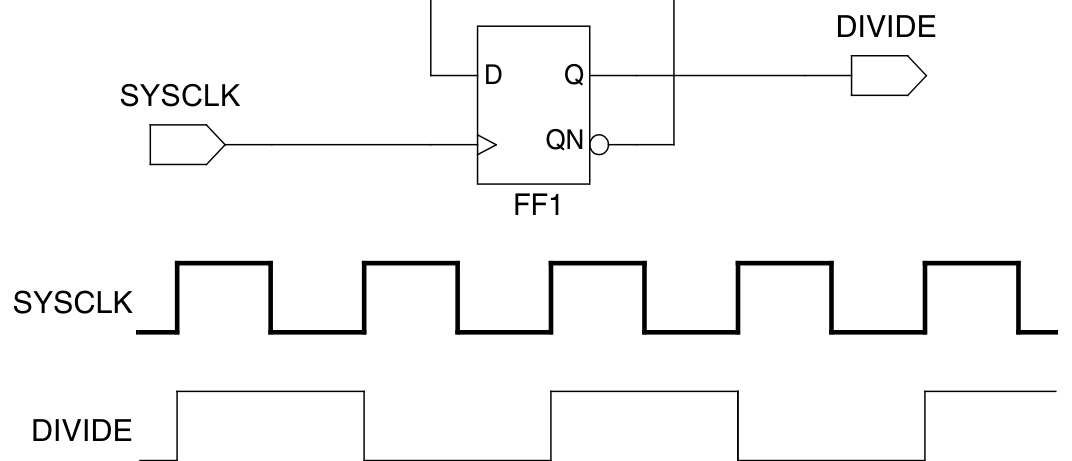
\includegraphics[width=0.85\textwidth]{fig-2-1.png}
  \caption{二分频时钟发生器}
  \label{fig:div2}
\end{figure}

工具不会从逻辑推导生成时钟的行为。必须用 \cmd{create\_generated\_clock}，按 master 时钟来说明生成时钟的行为，并指定：
\begin{itemize}
  \item 创建生成时钟所用的源对象（port、pin 或 net）。
  \item 用 \opt{-source} 指定 master 时钟的源。
  \item 用下列三种方法之一说明频率或波形如何从 master 时钟导出：
  \begin{itemize}
    \item 用 \opt{-divide\_by} 并给出分频因子，由 master 时钟频率除以该因子得到生成时钟频率。
    \item 用 \opt{-multiply\_by} 并给出倍频因子，由 master 时钟频率乘以该因子得到生成时钟频率。
    \item 用 \opt{-edges} 并列出要使用的 master 时钟边沿，按指定边沿导出波形。
  \end{itemize}
\end{itemize}

还可以：
\begin{itemize}
  \item 用 \opt{-name} 为生成时钟命名。若不命名，工具使用源对象列表中第一个对象的名称。
  \item 用 \opt{-add} 在同一生成时钟源对象上添加多个生成时钟。此时必须用 \opt{-master\_clock} 为附加生成时钟指定 master 时钟。
  \item 用 \opt{-combinational}，在计算生成时钟的 source latency 时只考虑生成时钟源与 master 时钟源之间的组合路径。默认情况下，时序分析同时考虑这两点之间的组合路径与时序路径。
  \item 对用 \opt{-divide\_by} 或 \opt{-multiply\_by} 创建的生成时钟，用 \opt{-invert} 反相波形。
  \item 对用 \opt{-multiply\_by} 创建的生成时钟，用 \opt{-duty\_cycle} 改变占空比。
  \item 对用 \opt{-edges} 从 master 时钟指定边沿导出的生成时钟，用 \opt{-edge\_shift} 延迟或平移所选边沿。
\end{itemize}

\subsection{生成时钟示例}
\subsubsection*{Generated Clock Examples}

下例创建两个生成时钟 \cmd{DIV2A} 与 \cmd{DIV2A\_INV}，频率为 master 时钟 \cmd{CLKA} 的一半。此外，\cmd{DIV2A\_INV} 的波形相对 master 时钟反相。
\begin{lstlisting}
icc2_shell> create_generated_clock -name DIV2A \
    -source [get_ports CLKA] -divide_by 2 \
    [get_pins U15/Q]
icc2_shell> create_generated_clock -name DIV2A_INV \
    -source [get_ports CLKA] -divide_by 2 -invert \
    [get_pins U15/QN]
\end{lstlisting}

下图给出该例中 master 时钟与生成时钟的波形。

\begin{figure}[htbp]
  \centering
  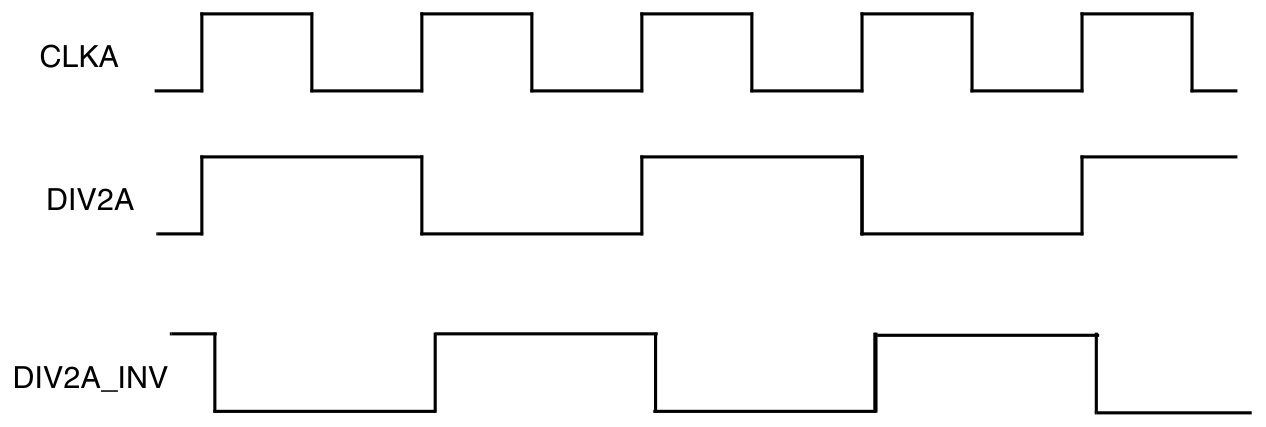
\includegraphics[width=0.9\textwidth]{fig-2-2.png}
  \caption{master 时钟与二分频生成时钟的波形}
  \label{fig:div2-wf}
\end{figure}

下例创建生成时钟 \cmd{MULT2B}，频率为 master 时钟 \cmd{CLKB} 的两倍，有效占空比为 75\%。
\begin{lstlisting}
icc2_shell> create_generated_clock -name MULT2B -duty_cycle 75 \
    -source [get_ports CLKB] -multiply_by 2 \
    [get_pins U29/GC]
\end{lstlisting}

\begin{figure}[htbp]
  \centering
  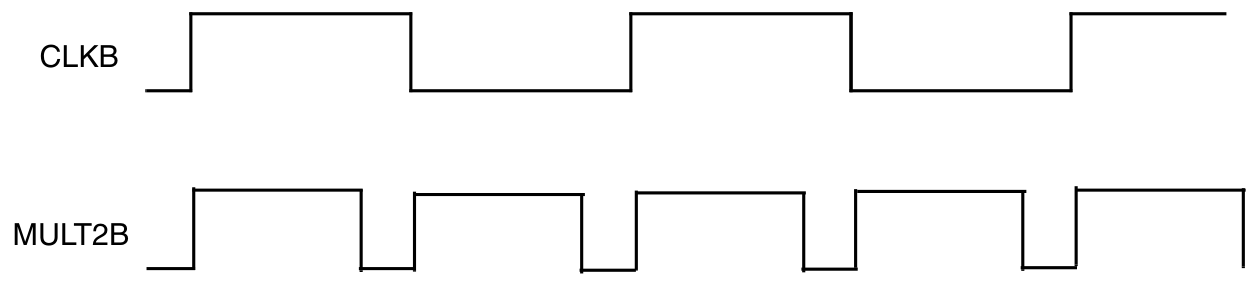
\includegraphics[width=0.9\textwidth]{fig-2-3.png}
  \caption{master 时钟与二倍频生成时钟的波形}
  \label{fig:mult2-wf}
\end{figure}

下例创建 master 时钟 \cmd{CLKC}，以及波形基于 master 时钟第 3、第 5 与第 9 个边沿、且每个边沿平移 2.2 个时间单位的生成时钟 \cmd{DIV3C}。
\begin{lstlisting}
icc2_shell> create_clock -period 2.2 -name CLKC [get_ports CLKC]
icc2_shell> create_generated_clock -name DIV3C \
    -edges {3 5 9} -edge_shift {2.2 2.2 2.2} \
    -source [get_ports SYSCLK] [get_pins U41/QN]
\end{lstlisting}

\cmd{report\_clocks} 按如下方式报告这些时钟：
\begin{lstlisting}
    p - propagated_clock
    G - Generated clock
Clock          Period   Waveform        Attrs     Sources
-------------------------------------------------------------
CLKC           2.20     {0 1.1}                   {CLKC}
DIV3C          6.60     {4.4 6.6}       G         {U41/Q}
Generated     Master       Generated    Waveform
Clock         Source       Source       Modification
-------------------------------------------------------------
DIV3C         MYCLK        U41/Q        edges( 3 5 9 )
                                        shifts( 2.2 2.2 2.2 )
\end{lstlisting}

\begin{figure}[htbp]
  \centering
  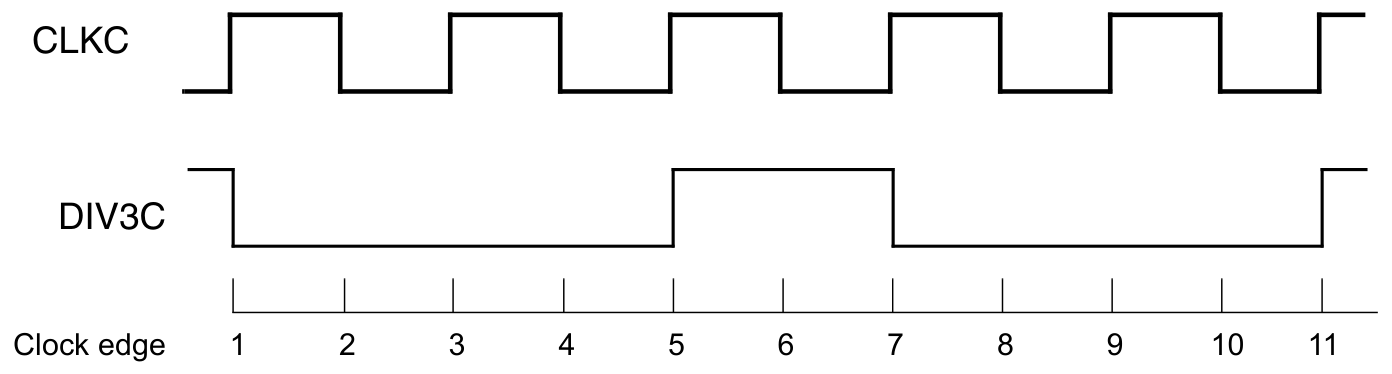
\includegraphics[width=0.92\textwidth]{fig-2-4.png}
  \caption{master 时钟与边沿平移后的三分频生成时钟波形}
  \label{fig:div3-wf}
\end{figure}

下例创建生成时钟 \cmd{CLKD\_INV}，并指定计算该生成时钟的 source latency 时，只使用生成时钟源与 master 时钟源之间的组合路径：
\begin{lstlisting}
icc2_shell> create_generated_clock -name CLKD_INV -divide_by 1 \
    -combinational -source [get_ports CLKD] [get_pins U52/Y]
\end{lstlisting}

下图给出该例中生成时钟源与 master 时钟源之间的全部可用路径。

\begin{figure}[htbp]
  \centering
  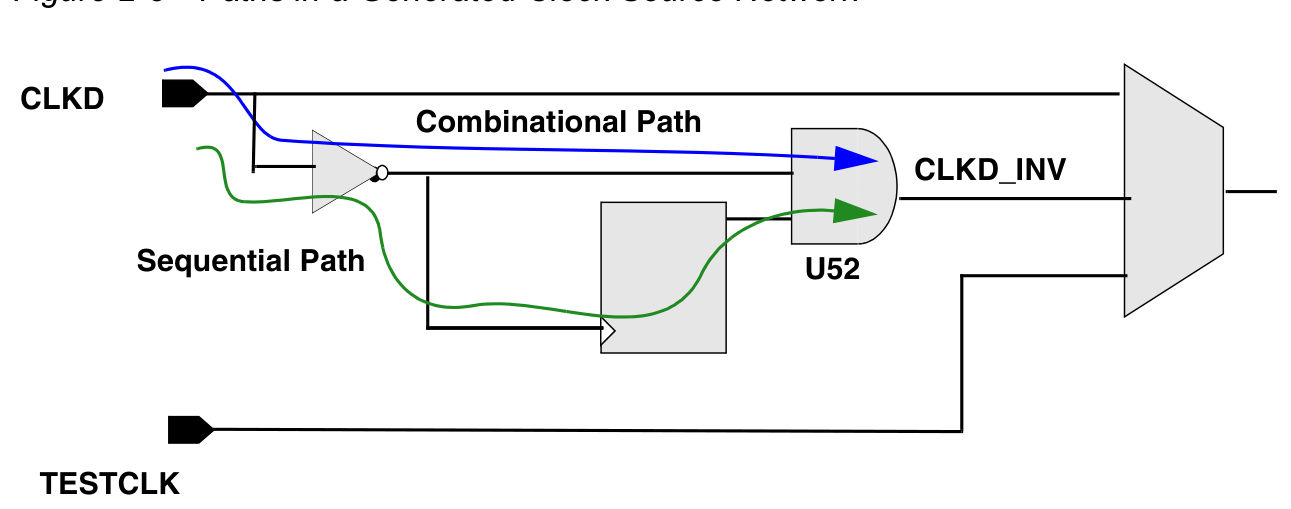
\includegraphics[width=0.85\textwidth]{fig-2-5.png}
  \caption{生成时钟源网络中的路径}
  \label{fig:gen-src-paths}
\end{figure}

\section{时钟网络效应}
\subsection*{Clock Network Effects}

时钟网络具有下列特性。

\begin{itemize}
  \item \textbf{Latency}\\
        时钟信号从原始时钟源传播到设计中时序单元所经历的时间。Latency 由两部分组成：
  \begin{itemize}
    \item Source latency：从时钟源到设计中时钟定义引脚的延迟。
    \item Network latency：从时钟定义点到寄存器时钟引脚的延迟。
  \end{itemize}
        表示 network latency 有两种方法：
  \begin{itemize}
    \item 估计并显式指定每个时钟的 latency。这称为理想网络延迟（ideal network latency），对应时钟称为理想时钟。理想时钟通常用在时钟树综合之前。
    \item 让工具沿时钟网络传播延迟来计算 latency。这称为传播网络延迟（propagated network latency），对应时钟称为传播时钟。传播时钟应只在时钟树综合之后使用。
  \end{itemize}
  \item \textbf{Uncertainty}\\
        同一时钟或不同时钟在寄存器时钟引脚上到达时间的最大变化。时钟不确定性有两个分量：
  \begin{itemize}
    \item 时钟抖动（jitter）：相对理想波形，源时钟相继边沿在产生时刻上的变化。
    \item 时钟偏斜（skew）：从 block 的时钟源到不同寄存器时钟引脚的传播延迟不同，所造成的到达时间差。这只适用于时钟树综合之前。时钟树综合之后，skew 已由传播时钟网络延迟计入。
  \end{itemize}
  \item \textbf{Transition time}\\
        信号从逻辑低变到逻辑高（上升时间）或从逻辑高变到逻辑低（下降时间）所需的时间。
\end{itemize}

下图给出时钟网络的时序效应。

\begin{figure}[htbp]
  \centering
  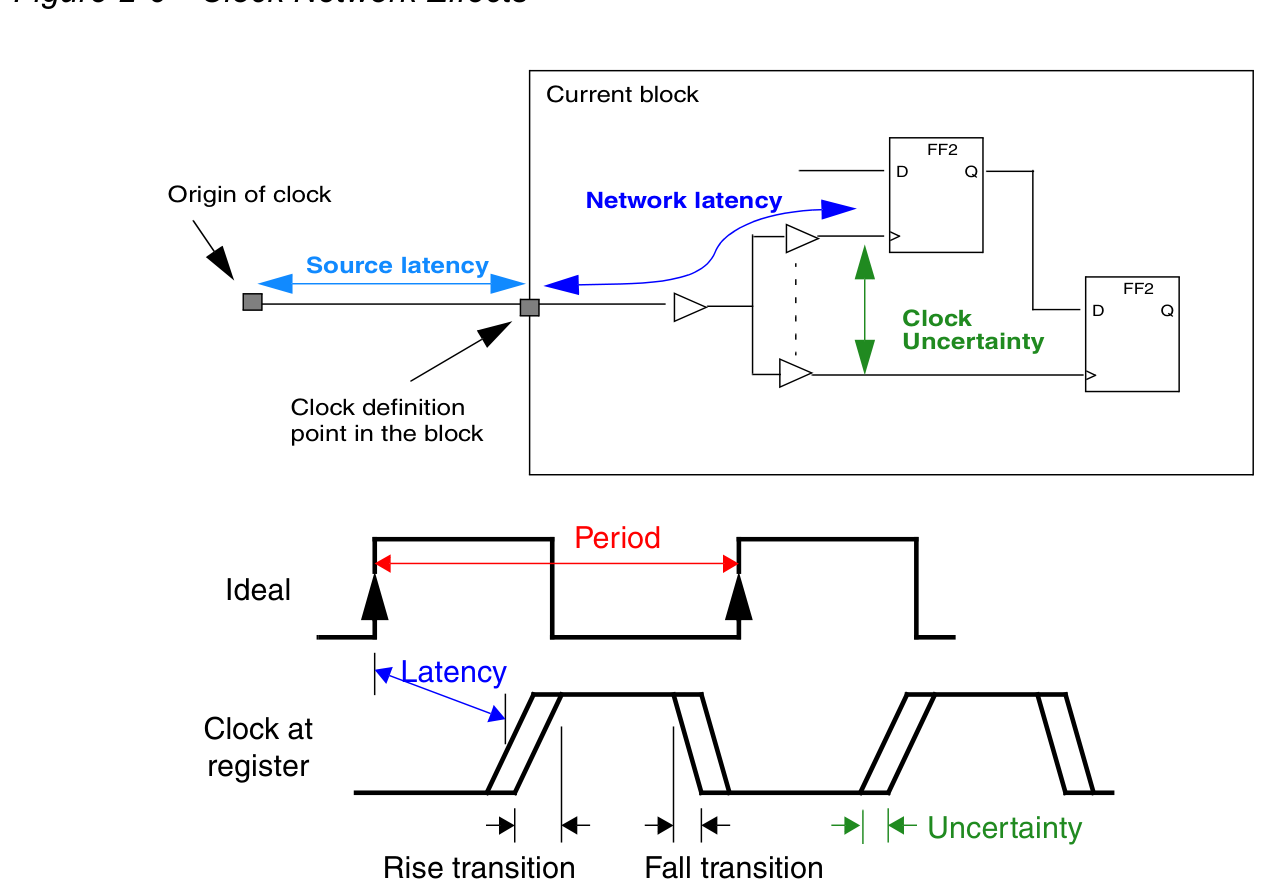
\includegraphics[width=0.88\textwidth]{fig-2-6.png}
  \caption{时钟网络效应}
  \label{fig:clk-net-effects}
\end{figure}

\section{指定时钟源端延迟}
\subsection*{Specifying Clock Source Latency}

对理想时钟与传播时钟都可用 \cmd{set\_clock\_latency -source} 设置 source latency，并指定：
\begin{itemize}
  \item 延迟值。
  \item 受影响的对象列表，可以包含一个或多个时钟、端口或引脚。若对象是 pin 或 port，必须用 \opt{-clock} 指定与该理想网络延迟关联的时钟。
\end{itemize}

还可以指定：
\begin{itemize}
  \item 用 \opt{-early} 与 \opt{-late} 给出 source latency 的 early / late 变化。工具对约束时钟所钟控的每个起点与终点，采用最严的 source latency（early 或 late）。setup 检查对每个起点用 late、对每个终点用 early；hold 检查对每个起点用 early、对每个终点用 late，如下图所示。
\end{itemize}

\begin{figure}[htbp]
  \centering
  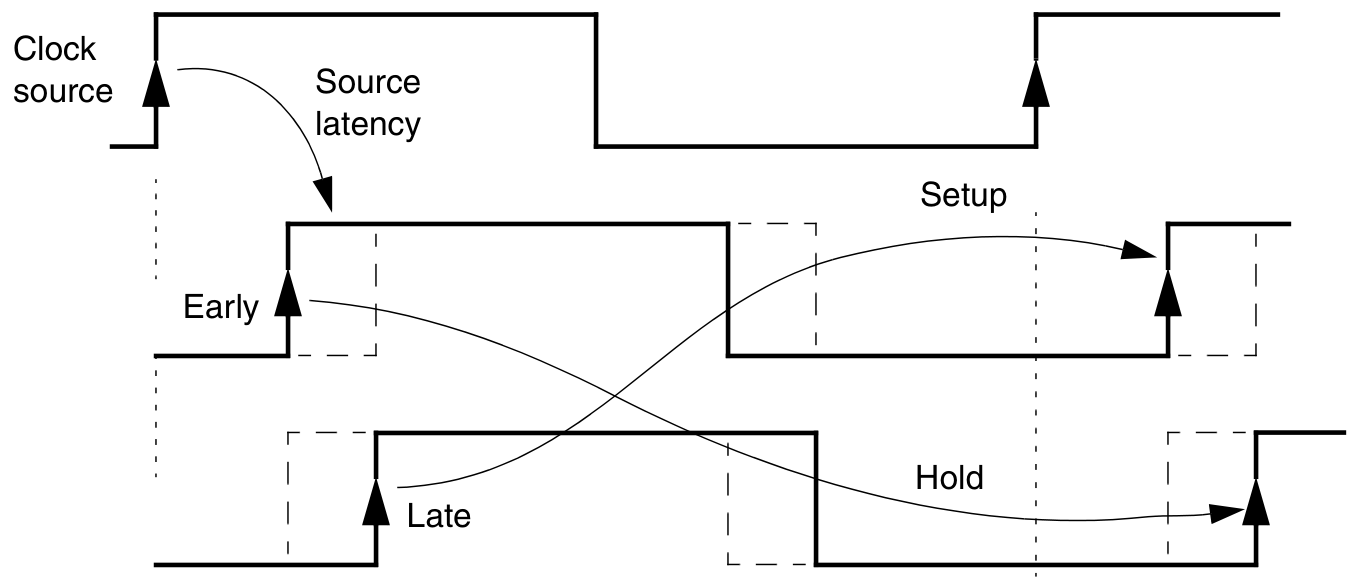
\includegraphics[width=0.85\textwidth]{fig-2-7.png}
  \caption{early 与 late 源端延迟波形}
  \label{fig:early-late-lat}
\end{figure}

\begin{itemize}
  \item 用 \opt{-dynamic} 给出 source latency 的动态变化分量，即相继时钟周期之间不同的那一部分。
\end{itemize}

对多 scenario 设计，source latency 默认只作用于当前 scenario。还可以：
\begin{itemize}
  \item 用 \opt{-modes} 指定某个 mode 的全部 scenario。
  \item 用 \opt{-corners} 指定指定 corner 与当前 mode 的全部 scenario。
  \item 同时用 \opt{-modes} 与 \opt{-corners} 指定指定 mode 与 corner 的全部 scenario。
  \item 用 \opt{-scenarios} 指定具体 scenario。使用该选项时不能再用 \opt{-modes} 或 \opt{-corners}。
\end{itemize}

下列命令把时钟 \cmd{CLK1} 的 source latency 指定为外部时钟网络延迟在 1.5 到 2.5 之间变化，动态分量为 0.5：
\begin{lstlisting}
icc2_shell> set_clock_latency 1.5 -source -early -dynamic 0.5 \
    [get_clocks CLK1]
icc2_shell> set_clock_latency 2.5 -source -late -dynamic 0.5 \
    [get_clocks CLK1]
\end{lstlisting}

用 \cmd{remove\_clock\_latency} 去掉由 \cmd{set\_clock\_latency} 指定的 source latency。

\section{指定理想网络延迟}
\subsection*{Specifying Ideal Network Latency}

用 \cmd{set\_ideal\_network} 把时钟指定为理想时钟。在完成时钟树综合之前，把所有时钟都指定为理想时钟。

用 \cmd{set\_clock\_latency} 指定理想网络延迟，并给出：
\begin{itemize}
  \item 延迟值。
  \item 受影响的对象列表，可以包含一个或多个时钟、端口或引脚。若对象是 pin 或 port，必须用 \opt{-clock} 指定关联时钟。
\end{itemize}

若在时钟网络的某个 pin 或 port 上指定了理想 latency，同时又在对应时钟对象上指定了 latency，则 pin 或 port 上的值作用于其扇出中的全部寄存器时钟引脚，并覆盖加在时钟对象上的 latency。

还可以把理想网络延迟限制为：
\begin{itemize}
  \item 只用 \opt{-rise} 或 \opt{-fall} 作用于上升沿或下降沿。否则同时作用于两个沿。
  \item 只用 \opt{-min} 或 \opt{-max} 作用于最小或最大工作条件。否则作用于全部工作条件。
\end{itemize}

对多 scenario 设计，理想时钟 latency 默认只作用于当前 scenario。指定范围的方式与 source latency 相同：\opt{-modes}、\opt{-corners}、两者同时，或 \opt{-scenarios}。使用 \opt{-scenarios} 时不能再用 \opt{-modes} 或 \opt{-corners}。

下例为当前设计中名为 \cmd{CLK1} 的时钟把期望的上升 latency 设为 1.2、下降 latency 设为 0.9：
\begin{lstlisting}
icc2_shell> set_clock_latency -rise 1.2 [get_clocks CLK1]
icc2_shell> set_clock_latency -fall 0.9 [get_clocks CLK1]
\end{lstlisting}

用 \cmd{remove\_clock\_latency} 去掉由 \cmd{set\_clock\_latency} 指定的理想网络延迟。

\section{指定时钟不确定性}
\subsection*{Specifying Clock Uncertainty}

用 \cmd{set\_clock\_uncertainty} 指定时钟不确定性，给出不确定性数值以及下列之一：
\begin{itemize}
  \item 简单不确定性或抖动：同一时钟相继边沿之间的不确定性。对象列表由时钟、端口或引脚组成。简单不确定性作用于所指定时钟、端口或引脚扇出中的全部寄存器时钟引脚。
  \item 两个时钟之间的时钟间不确定性（interclock uncertainty），用下列方法之一：
  \begin{itemize}
    \item 用 \opt{-from}、\opt{-rise\_from} 或 \opt{-fall\_from} 指定源时钟。
    \item 用 \opt{-to}、\opt{-rise\_to} 或 \opt{-fall\_to} 指定目的时钟。
  \end{itemize}
        指定两个时钟之间的 interclock uncertainty 时，若既有从第一个时钟到第二个时钟的路径，也有反方向路径，即使数值相同，也必须为两个方向都指定不确定性。
\end{itemize}

\begin{figure}[htbp]
  \centering
  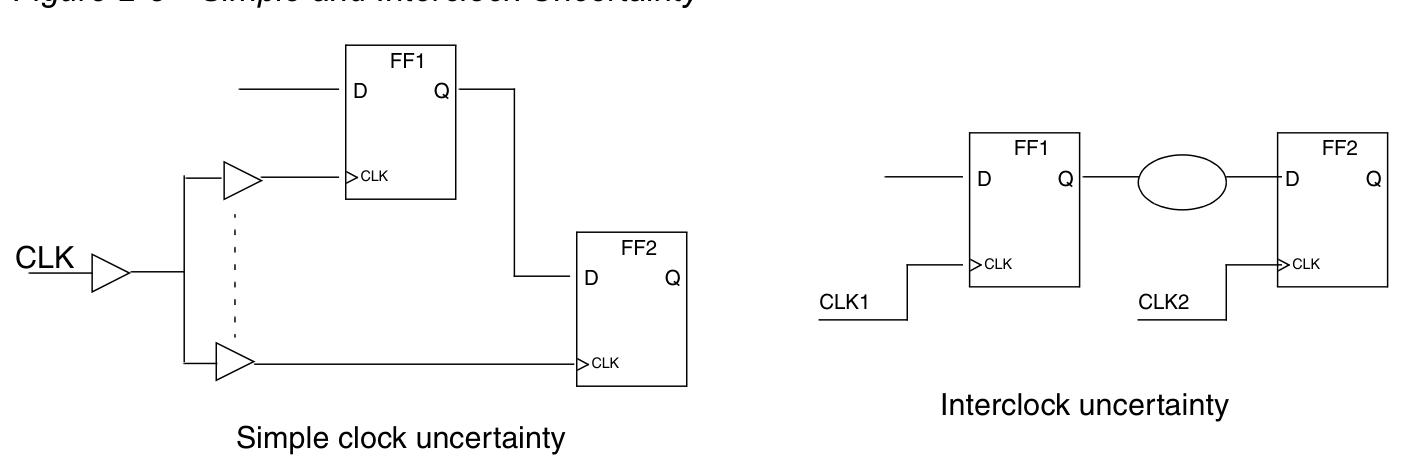
\includegraphics[width=0.92\textwidth]{fig-2-8.png}
  \caption{简单不确定性与时钟间不确定性}
  \label{fig:uncertainty}
\end{figure}

还可以：
\begin{itemize}
  \item 用 \opt{-setup} 指定 setup 检查的简单或时钟间不确定性。
  \item 用 \opt{-hold} 指定 hold 检查的不确定性。
\end{itemize}

对多 scenario 设计，时钟不确定性默认只作用于当前 scenario。指定范围同样使用 \opt{-modes}、\opt{-corners}、两者同时，或 \opt{-scenarios}。使用 \opt{-scenarios} 时不能再用 \opt{-modes} 或 \opt{-corners}。

例如，对由时钟 \cmd{CLK1} 钟控的终点，把简单 setup 不确定性设为 0.21、hold 不确定性设为 0.33：
\begin{lstlisting}
icc2_shell> set_clock_uncertainty -setup 0.21 [get_clocks CLK1]
icc2_shell> set_clock_uncertainty -hold 0.33 [get_clocks CLK1]
\end{lstlisting}

把时钟 \cmd{CLKA} 与 \cmd{CLKB} 之间的 interclock uncertainty 设为 2（setup 与 hold 都设置）：
\begin{lstlisting}
icc2_shell> set_clock_uncertainty 2 -from [get_clocks CLKA] \
    -to [get_clocks CLKB]
icc2_shell> set_clock_uncertainty 2 -from [get_clocks CLKB] \
    -to [get_clocks CLKA]
\end{lstlisting}

用 \cmd{remove\_clock\_uncertainty} 去掉时钟不确定性设置。

\section{指定理想时钟转换时间}
\subsection*{Specifying Ideal Clock Transition}

理想时钟的默认转换时间为零。要用 \cmd{set\_clock\_transition} 为理想时钟指定非零转换时间，并给出：
\begin{itemize}
  \item 理想转换时间值。
  \item 它作用的时钟列表。
\end{itemize}

还可以限定转换时间只作用于：
\begin{itemize}
  \item 用 \opt{-rise} 或 \opt{-fall} 指定的上升沿或下降沿。
  \item 用 \opt{-min} 或 \opt{-max} 指定的最小或最大条件。
\end{itemize}

对多 scenario 设计，理想时钟转换时间默认只作用于当前 scenario。范围选项与前面相同：\opt{-modes}、\opt{-corners}、两者同时，或 \opt{-scenarios}。

工具把所指定的转换时间用于这些时钟传递扇出中的全部寄存器时钟引脚。

例如，在当前 scenario 中，把时钟 \cmd{CLK1} 全部寄存器时钟引脚上的转换时间指定为 0.64：
\begin{lstlisting}
icc2_shell> set_clock_transition 0.64 [get_clocks CLK1]
\end{lstlisting}

用 \cmd{remove\_clock\_transition} 去掉该命令指定的理想转换时间。

\section{为理想时钟启用 clock-to-data 分析}
\subsection*{Enabling Clock-to-Data Analysis for Ideal Clocks}

若时钟到达某个不是时钟引脚（时序引脚）的单元引脚，如下图所示，工具把它识别为 clock-to-data 引脚，并把引脚属性 \cmd{pin\_is\_clock\_to\_data} 设为 \cmd{true}。

\begin{figure}[htbp]
  \centering
  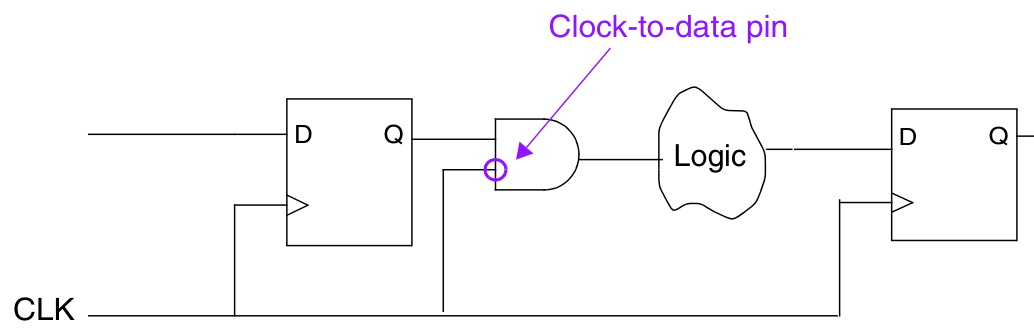
\includegraphics[width=0.72\textwidth]{fig-2-9.png}
  \caption{clock-to-data 引脚}
  \label{fig:c2d}
\end{figure}

可用下列命令找出 block 中的 clock-to-data 引脚：
\begin{lstlisting}
icc2_shell> get_pins -filter "pin_is_clock_to_data==true"
\end{lstlisting}

若传播时钟到达 clock-to-data 引脚，工具把传播时钟到达时间用作该引脚的数据到达时间，把传播时钟转换时间用作数据转换时间。

理想时钟到达 clock-to-data 引脚时，默认不把理想时钟 latency 用作数据到达时间，也不把理想时钟转换时间用作数据转换时间。要把理想时钟的 latency 与转换时间用到该引脚上，把应用选项 \appopt{time.enable\_clock\_to\_data\_analysis} 设为 \cmd{true}。

\section{时钟的单边性}
\subsection*{Unateness of Clocks}

时钟信号分为：
\begin{itemize}
  \item \textbf{Positive unate}：时钟源的上升沿只能在寄存器时钟引脚上引起上升沿，下降沿只能引起下降沿。
  \item \textbf{Negative unate}：时钟源的上升沿只能在寄存器时钟引脚上引起下降沿，下降沿只能引起上升沿。也就是说，时钟信号被反相。
  \item \textbf{Non-unate}：时钟路径中存在 non-unate 时序弧，时钟极性不明确。例如经过 XOR 门的时钟不是 unate 的。极性是正还是负，取决于 XOR 另一输入的状态。
\end{itemize}

下图给出产生 unate 与 non-unate 时钟信号的时钟逻辑示例。

\begin{figure}[htbp]
  \centering
  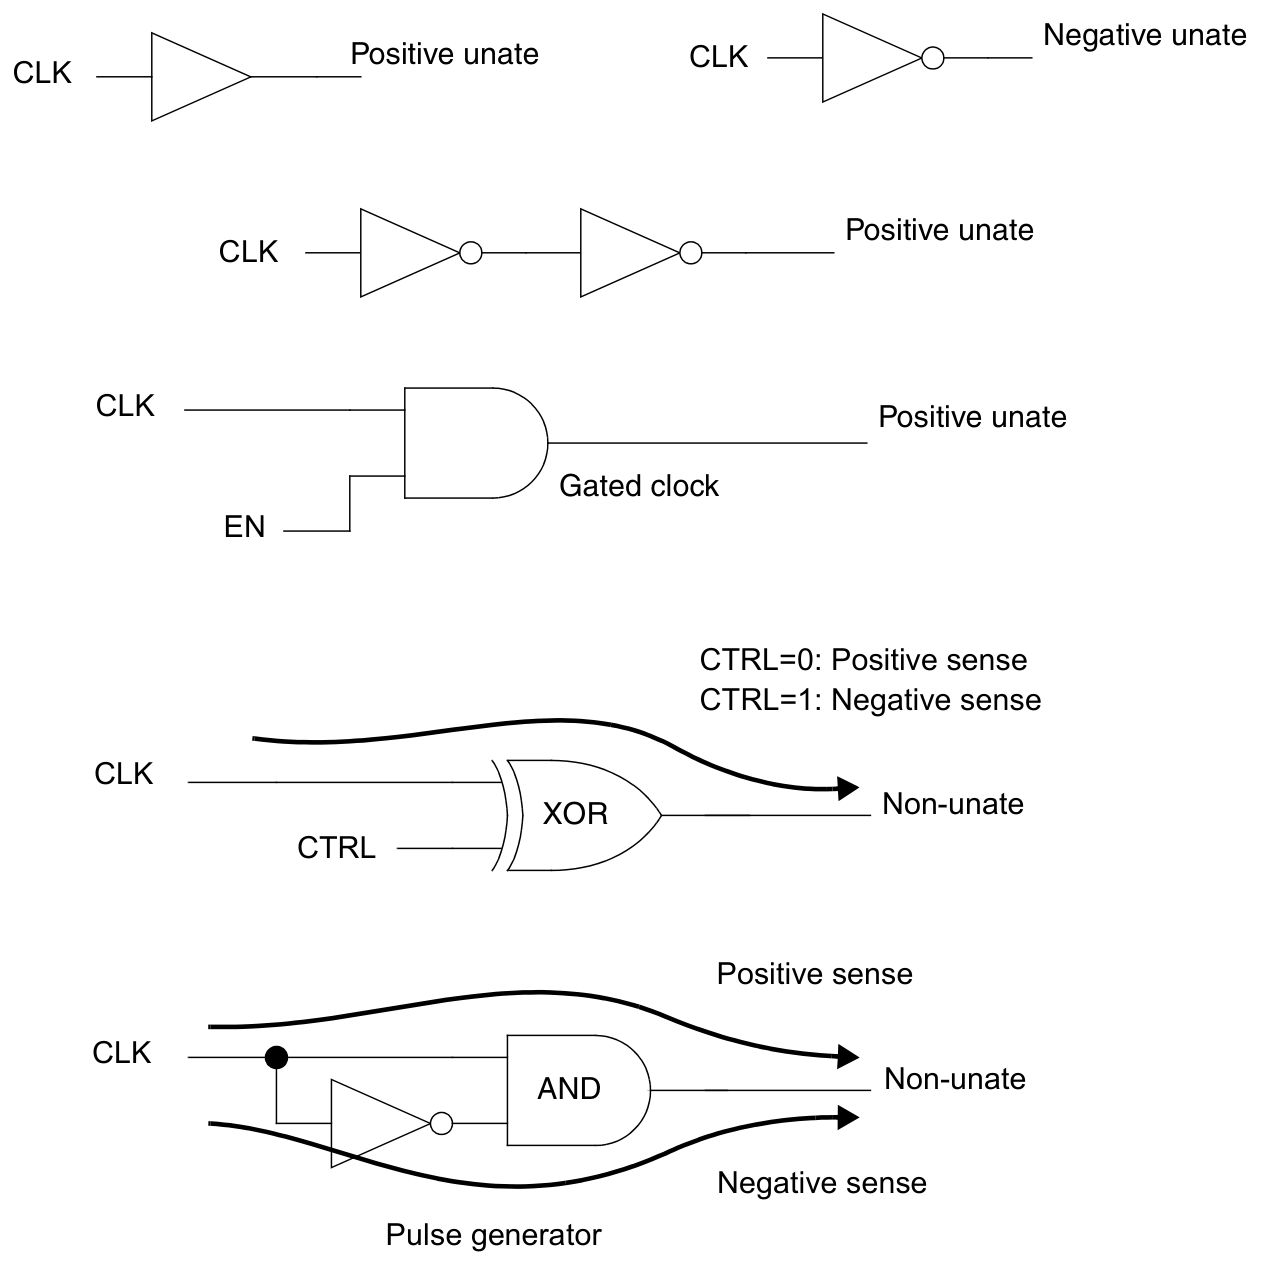
\includegraphics[width=0.82\textwidth]{fig-2-10.png}
  \caption{unate 与 non-unate 时钟信号}
  \label{fig:unate}
\end{figure}

\section{传播指定的时钟极性}
\subsection*{Propagating a Specific Clock Sense}

若时钟网络只含产生 positive unate 或 negative unate 时钟信号的逻辑，工具可以推导到达每个寄存器时钟引脚的时钟极性。若时钟网络含有产生 non-unate 时钟信号的逻辑，可以用 \cmd{set\_sense} 只传播时钟的某一种极性，以消除这种歧义：
\begin{itemize}
  \item 用 \opt{-positive} 让某一点之后只传播正极性。
  \item 用 \opt{-negative} 让某一点之后只传播负极性。
\end{itemize}

也可以用 \cmd{set\_sense} 阻止时钟越过某一点继续传播：
\begin{itemize}
  \item 用 \opt{-clock\_leaf} 阻止时钟越过该点，并把该点视为时钟 sink。因为该点被当作时钟 sink，工具会：
  \begin{itemize}
    \item 把扇入该点的路径上引脚的 \cmd{is\_clock\_used\_as\_clock} 属性设为 \cmd{true}；
    \item 相对该点做时钟门控检查。
  \end{itemize}
  \item 用 \opt{-stop\_propagation} 阻止时钟越过该点，但不把它视为时钟 sink。因此工具不会设置 \cmd{is\_clock\_used\_as\_clock}，也不会相对该点做时钟门控检查。
\end{itemize}

\opt{-positive}、\opt{-negative}、\opt{-logical\_stop\_propagation} 与 \opt{-stop\_propagation} 互斥。

若多个时钟都能到达所指定的引脚，可用 \opt{-clocks} 把设置限制到某些时钟。

用 \cmd{remove\_clock\_sense} 撤销 \cmd{set\_sense} 的效果。

下例让名为 \cmd{CLK1} 的时钟在单元引脚 \cmd{U29/z} 之后只传播正极性，让 \cmd{CLK2} 只传播负极性：
\begin{lstlisting}
icc2_shell> set_sense -positive \
    -clocks [get_clocks CLK1] [get_pins U29/z]
icc2_shell> set_sense -negative \
    -clocks [get_clocks CLK2] [get_pins U29/z]
\end{lstlisting}

下例阻止全部时钟（既作为时钟也作为数据）越过引脚 \cmd{U32/z} 继续传播：
\begin{lstlisting}
icc2_shell> set_sense -stop_propagation [get_pins U32/z]
\end{lstlisting}

\section{创建脉冲时钟}
\subsection*{Creating Pulse Clocks}

脉冲时钟（pulse clock）常用于提高性能并降低功耗。它由一串短脉冲组成，脉冲的上升沿与下降沿都由另一时钟的同一个边沿触发。

要分析含脉冲时钟的电路，工具需要该时钟的时序特性。可以使用已在 \cmd{.lib} 库描述中完成特性化的脉冲发生器单元。此时不必再额外指定脉冲时钟特性。关于在库单元上指定脉冲发生器特性，见 Library Compiler 文档。

若库中没有已特性化的脉冲发生器单元，必须在设计中每个脉冲产生点用下列方法之一指定脉冲时钟特性：
\begin{itemize}
  \item 用 \cmd{create\_generated\_clock} 相对源时钟描述脉冲时序。这会在脉冲产生点创建一个新的时钟域。
  \item 用 \cmd{set\_sense} 指定所产生脉冲相对源时钟的极性。这不创建新时钟域，只为该点下游已有时钟指定极性。
\end{itemize}

\subsection{用 create\_generated\_clock 创建脉冲时钟}
\subsubsection*{Creating a Pulse Clock With the create\_generated\_clock Command}

可以把 \opt{-edges} 与 \cmd{create\_generated\_clock} 一起用来创建脉冲时钟。使用 \opt{-edges} 时：
\begin{itemize}
  \item 重复数字所在的位置决定产生的是高有效还是低有效脉冲。
  \item 被重复的边沿编号决定用 master 时钟的哪一种边沿来触发脉冲。
\end{itemize}

例如：
\begin{itemize}
  \item 源时钟上升沿触发高脉冲：\opt{-edges \{1 1 3\}}。
  \item 源时钟下降沿触发高脉冲：\opt{-edges \{2 2 4\}}。
  \item 源时钟上升沿触发低脉冲：\opt{-edges \{1 3 3\}}。
  \item 源时钟下降沿触发低脉冲：\opt{-edges \{2 4 4\}}。
\end{itemize}

用重复的边沿编号把生成时钟指定为脉冲时钟，可以保证源时钟与脉冲时钟之间的延迟检查正确。

考虑下图中的脉冲时钟电路。源时钟的边沿编号 1 同时触发脉冲时钟的上升沿与下降沿。脉冲宽度由反相器的延迟决定。

\begin{figure}[htbp]
  \centering
  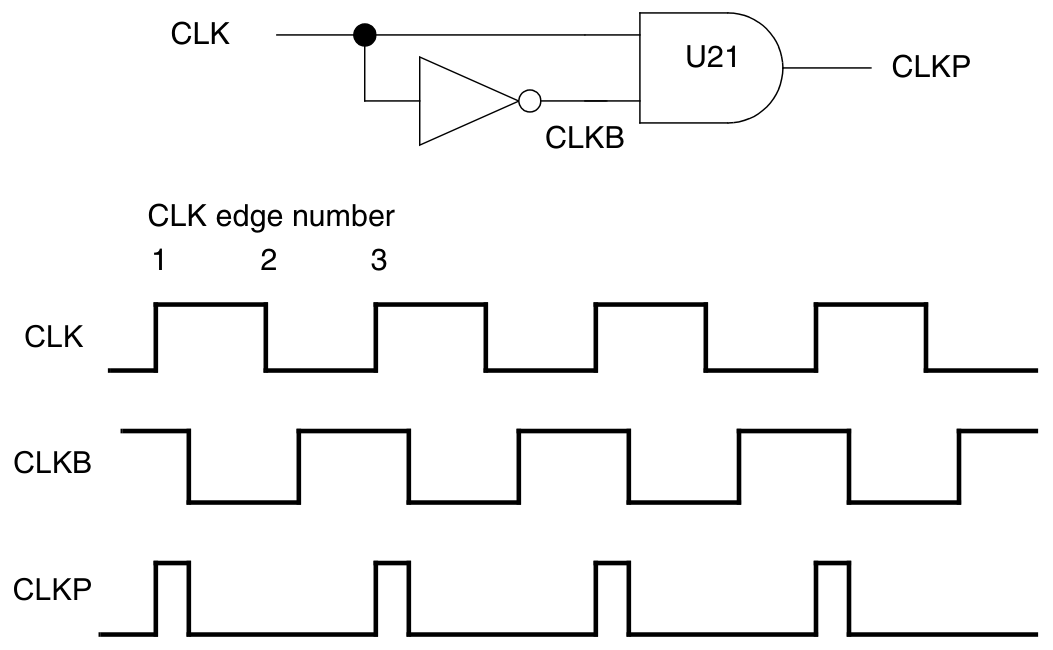
\includegraphics[width=0.78\textwidth]{fig-2-11.png}
  \caption{指定为生成时钟的脉冲时钟}
  \label{fig:pulse}
\end{figure}

把生成脉冲时钟 \cmd{CLKP} 指定为生成时钟：
\begin{lstlisting}
icc2_shell> create_generated_clock -name CLKP -source CLK \
    -edges {1 1 3} [get_pins U21/z]
\end{lstlisting}

\subsection{用 set\_sense 定义脉冲时钟}
\subsubsection*{Defining a Pulse Clock With the set\_sense Command}

可以用 \cmd{set\_sense} 的 \opt{-pulse} 把已有时钟指定为脉冲时钟：
\begin{itemize}
  \item 上升沿触发的高脉冲：\opt{-pulse rise\_triggered\_high\_pulse}。
  \item 上升沿触发的低脉冲：\opt{-pulse rise\_triggered\_low\_pulse}。
  \item 下降沿触发的高脉冲：\opt{-pulse fall\_triggered\_high\_pulse}。
  \item 下降沿触发的低脉冲：\opt{-pulse fall\_triggered\_low\_pulse}。
\end{itemize}

脉冲时钟不定义为单独的时钟域。只是源时钟的指定极性从时钟网络中该点向下游传播。

下列命令指定单元 \cmd{U21} 输出上的时钟是一个在源时钟上升沿既上升又下降的脉冲：
\begin{lstlisting}
prompt> set_sense -pulse rise_triggered_high_pulse \
    [get_pins U21/z]
\end{lstlisting}

\subsection{指定脉冲时钟的标称宽度}
\subsubsection*{Specifying the Nominal Width of a Pulse Clock}

无论使用库中定义的脉冲发生器单元、\cmd{create\_generated\_clock} 还是 \cmd{set\_sense}，所产生脉冲的标称宽度都是零。要得到实际脉冲宽度，工具考虑脉冲发生器输出引脚上上升与下降 latency 的差异：
\begin{quote}
（高脉冲宽度）=（下降 network latency）$-$（上升 network latency）\\
（低脉冲宽度）=（上升 network latency）$-$（下降 network latency）
\end{quote}

可以用 \cmd{set\_clock\_latency} 为理想时钟显式指定 latency（从而指定脉冲宽度），也可以让工具为传播时钟从电路计算传播 latency。

例如，要把单元 \cmd{U21} 输出下游全部寄存器的高脉冲理想宽度设为 0.5，且总 latency 为 0.6：
\begin{lstlisting}
icc2_shell> set_clock_latency -rise 0.6 [get_pins and2.z]
icc2_shell> set_clock_latency -fall 1.1 [get_pins and2.z]
\end{lstlisting}

\section{设置并报告最小脉冲宽度约束}
\subsection*{Setting and Reporting Minimum Pulse Width Constraints}

由于上升沿与下降沿传播延迟不同，寄存器处的时钟脉冲宽度可能变窄。若寄存器时钟引脚上的脉冲过窄，寄存器可能无法正确采集数据。因此，满足最小脉冲宽度约束是时序电路正确工作所必需的。

库单元引脚可以定义最小脉冲宽度。此外，可以用 \cmd{set\_min\_pulse\_width} 为指定时钟或时钟引脚显式设置脉冲宽度约束。

默认同时约束时钟的高脉冲与低脉冲。若只约束高脉冲或低脉冲，使用 \opt{-high} 或 \opt{-low}。

下例把 \cmd{reg1/CK} 上时钟信号的高、低最小脉冲宽度分别设为 0.6 与 1.0：
\begin{lstlisting}
set_min_pulse_width -high 0.6 reg1/CK
set_min_pulse_width -low 1.0 reg1/CK
\end{lstlisting}

用 \cmd{report\_min\_pulse\_width} 或 \cmd{report\_constraints -min\_pulse\_width} 检查脉冲宽度违例。
\begin{lstlisting}
icc2_shell> report_min_pulse_width
...
                    Required      Actual
  Pin               pulse width   pulse width   Slack
  -----------------------------------------------------
 reg1/CK(low)        1.00          0.87         -0.13
 reg1/CK(high)       0.60          1.13          0.53
\end{lstlisting}

用 \cmd{remove\_min\_pulse\_width} 去掉这些约束。

\section{定义时钟组之间的关系}
\subsection*{Defining the Relationship Between Clock Groups}

对多时钟设计，时序分析默认检查所有时钟之间的时序路径。若某些时钟之间没有交互，可用 \cmd{set\_clock\_groups} 说明这一点，从而缩短时序分析的运行时间。

使用 \cmd{set\_clock\_groups} 时必须指定：
\begin{itemize}
  \item 时钟组之间的关系，为下列之一：
  \begin{itemize}
    \item \opt{-physically\_exclusive}：物理互斥。工具假定这些时钟组在设计中不同时存在，因此不检查它们之间的时序路径，也不在这些时钟组的网线之间做串扰分析。
    \item \opt{-logically\_exclusive}：逻辑互斥。工具假定这些时钟组之间没有相位关系，因此不检查时钟之间的时序路径，但仍在这些时钟组的网线之间做串扰分析。
    \item \opt{-asynchronous}：异步。工具假定这些时钟组之间没有相位关系，因此不检查时钟之间的时序路径，但仍用无限到达时间窗口在这些时钟组的网线之间做串扰分析。
  \end{itemize}
  \item 用 \opt{-group} 一次或多次指定一个或多个时钟组。
  \begin{itemize}
    \item 只指定一次时，工具假定该组中的时钟与设计中所有其他时钟之间具有所指定的关系。
    \item 指定两次或更多次时，工具假定每一对时钟组之间具有所指定的关系。
  \end{itemize}
\end{itemize}

还可以：
\begin{itemize}
  \item 用 \opt{-name} 为时钟分组命名。若不命名，工具为每个分组推导一个唯一名称。
  \item 对用 \opt{-asynchronous} 指定的异步分组，用 \opt{-allow\_paths} 允许指定时钟之间仍做时序分析。
\end{itemize}

用 \cmd{remove\_clock\_groups} 去掉由 \cmd{set\_clock\_groups} 声明的时钟分组。

例如，指定时钟 \cmd{CK1} 相对设计中所有其他时钟物理互斥：
\begin{lstlisting}
icc2_shell> set_clock_groups -physically_exclusive -group {CK1}
\end{lstlisting}

指定时钟 \cmd{CK2}、\cmd{CK3} 与时钟 \cmd{CK4}、\cmd{CK5} 逻辑互斥：
\begin{lstlisting}
icc2_shell> set_clock_groups -logically_exclusive \
    -group {CK2 CK3} -group {CK4 CK5}
\end{lstlisting}

指定时钟 \cmd{CK6}、\cmd{CK7} 与 \cmd{CK8} 彼此异步：
\begin{lstlisting}
icc2_shell> set_clock_groups -asynchronous \
    -group {CK6} -group {CK7} -group {CK8}
\end{lstlisting}

\section{报告时钟相关信息}
\subsection*{Reporting Clock Related Information}

用 \cmd{report\_clocks} 报告由 \cmd{create\_clock} 与 \cmd{create\_generated\_clock} 定义的时钟。默认报告：
\begin{itemize}
  \item 全部时钟的周期、波形、属性与源。
  \item 全部生成时钟的 master 时钟源、master 时钟名以及波形修改方式。
\end{itemize}

还可以报告：
\begin{itemize}
  \item 通过指定时钟名，只报告所选时钟。
  \item 用 \opt{-skew} 报告理想时钟网络特性，包括用 \cmd{set\_clock\_latency} 指定的 source 与 network latency、用 \cmd{set\_clock\_uncertainty} 指定的不确定性，以及用 \cmd{set\_clock\_transition} 指定的理想转换时间。
  \item 用 \opt{-groups} 报告由 \cmd{set\_clock\_groups} 指定的时钟分组。
  \item 用 \opt{-modes} 报告所选 mode 的时钟信息。
\end{itemize}

用 \cmd{get\_clocks} 或 \cmd{all\_clocks} 创建时钟 collection。时钟对象与同名端口对象要用 \cmd{get\_clocks} 与 \cmd{get\_ports} 区分。

例如，报告周期小于或等于 15.0 的时钟：
\begin{lstlisting}
icc2_shell> report_clocks [get_clocks -filter "period <= 15.0" *]
...
Attributes:
    d - dont_touch_network
    f - fix_hold
    p - propagated_clock
    G - generated_clock
Clock          Period   Waveform            Attrs     Sources
------------------------------------------------------------------------
PCI_CLK         15.00   {0 7.5}                       {pclk}
SDRAM_CLK        7.50   {0 3.75}                      {sdram_clk}
SD_DDR_CLK       7.50   {0 3.75}            G         {sd_CK}
SYS_CLK          8.00   {0 4}                         {sys_clk}
------------------------------------------------------------------------
Generated     Master         Generated      Master         Waveform
Clock         Source         Source         Clock          Modification
------------------------------------------------------------------------
SD_DDR_CLK    sdram_clk      {sd_CK}        SDRAM_CLK      divide_by(1)
------------------------------------------------------------------------
\end{lstlisting}

\section{删除时钟}
\subsection*{Removing Clocks}

\begin{itemize}
  \item 用 \cmd{remove\_clocks} 删除由 \cmd{create\_clock} 创建的真实时钟或虚拟时钟。
  \item 用 \cmd{remove\_generated\_clocks} 删除由 \cmd{create\_generated\_clock} 创建的生成时钟。
\end{itemize}

% 第 3 章 Constraining Timing Paths
\bichapter{约束时序路径}{Constraining Timing Paths}\label{chap:paths}

时序路径是设计中的一条点到点序列：从寄存器时钟引脚或输入端口出发，经过组合逻辑，结束于寄存器数据输入引脚或输出端口。

下列主题说明时序路径，以及约束时序路径的相关任务：
\begin{itemize}
  \item 时序路径与 path group
  \item 创建 path group
  \item 同一 launch 与 capture 时钟的路径延迟分析
  \item 不同 launch 与 capture 时钟的路径延迟分析
  \item 输入延迟与输出延迟简介
  \item 为端口设置输入延迟与输出延迟
  \item 指定时序例外
  \item 指定 false path 例外
  \item 指定最大与最小路径延迟例外
  \item 指定 multicycle path 例外
  \item 指定路径时序裕量例外
  \item 高效地指定例外
  \item 例外的优先级
  \item 禁用下层 block 内部的时序路径
  \item 使用 case analysis
  \item 禁用时序弧
  \item 使能 preset 与 clear 时序
  \item data-to-data check 简介
  \item 指定 data-to-data check
  \item 使能基于库的 data check
  \item 时钟门控检查简介
  \item 指定时钟门控检查
\end{itemize}

\section{时序路径与 path group}
\subsection*{Timing Paths and Path Groups}

IC Compiler II 分析并优化设计中的时序路径。每条路径都有：
\begin{itemize}
  \item 起点（startpoint），数据在此被发射（launch）。\\
        路径起点是时序单元的时钟引脚，或设计的输入端口。有效时钟沿到达起点时，数据沿该路径被发射出去。输入端口也可以视为起点，因为数据由外部源发射后到达该端口。
  \item 终点（endpoint），数据穿过组合逻辑后在此被捕获（capture）。\\
        路径终点是时序单元的数据输入引脚，或设计的输出端口。有效时钟沿到达捕获器件的时钟输入时，路径末端的数据被捕获。输出端口也可以视为终点，因为离开该端口的数据由外部电路捕获。
\end{itemize}

下图给出一个设计及其时序路径的例子。

\begin{figure}[htbp]
  \centering
  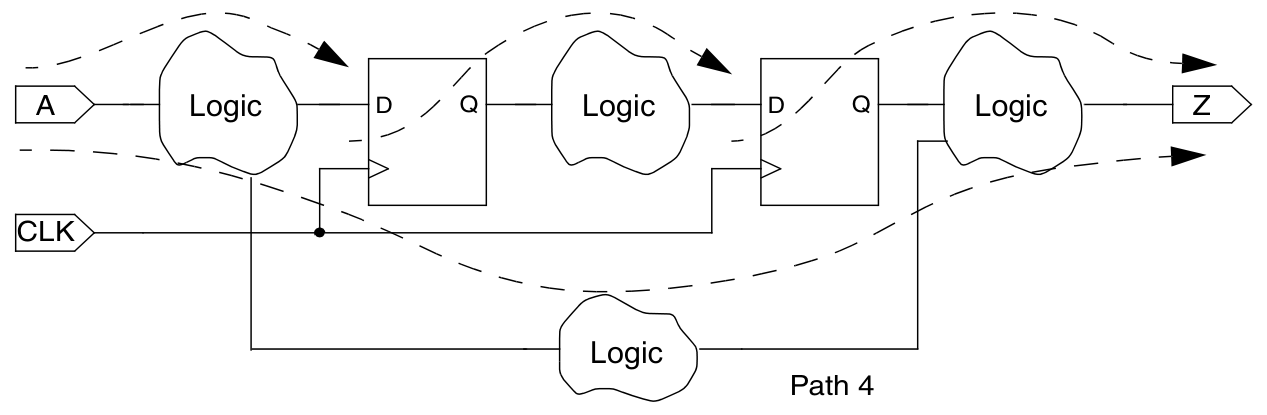
\includegraphics[width=0.9\textwidth]{fig-3-1.png}
  \caption{时序路径类型}
  \label{fig:3-1}
\end{figure}

每条路径都从数据发射点出发，经过若干组合逻辑，结束于数据捕获点：
\begin{itemize}
  \item 路径 1 从输入端口出发，结束于时序单元的数据输入。
  \item 路径 2 从时序单元的时钟引脚出发，结束于时序单元的数据输入。
  \item 路径 3 从时序单元的时钟引脚出发，结束于输出端口。
  \item 路径 4 从输入端口出发，结束于输出端口。
\end{itemize}

设计中的每条路径都有对应的时序裕量（slack）。slack 是时间值，可以为正、零或负。slack 最差的那一条路径称为关键路径（critical path）。它是负 slack 最大的路径；若没有时序违例，则是设计中全部路径里 slack 最小的那一条。

工具把时序路径组织成组，并按组分别做时序分析与优化。默认情况下，设计中的每个时钟对应一个 path group。终点由某个时钟打拍的全部时序路径，都属于该时钟的 path group。

工具还会创建一个名为 \cmd{**default**} 的 path group（名称中包含星号）。\cmd{**default**} 组收纳无法按终点所用时钟归类的路径，例如直通（feedthrough）路径与异步路径。

同一 path group 内的全部时序路径一起做时序优化，并从关键路径开始。

默认情况下，所有 path group 的权重相同；一组之内的路径与其他 path group 分开优化、分开报告。在每个 path group 内部，工具持续优化并改善关键路径的时序，直到组内另一条路径变得更加关键。

\section{创建 path group}
\subsection*{Creating Path Groups}

要改变 path group 中的路径，使用 \cmd{group\_path} 命令，方式如下：
\begin{itemize}
  \item 用 \opt{-name} 指定名称，创建新的 path group。
  \item 用 \opt{-name} 指定已有 path group 的名称，把路径加入该组。
  \item 用 \opt{-default} 把路径从当前 path group 移回它们所属的默认 path group。
\end{itemize}

用下列一种或多种方法标识时序路径：
\begin{itemize}
  \item 用 \opt{-from}、\opt{-rise\_from} 或 \opt{-fall\_from} 指定路径起点。
  \item 用 \opt{-through}、\opt{-rise\_through} 或 \opt{-fall\_through} 指定一个或多个经过点，这些选项可使用一次或多次。
  \item 用 \opt{-to}、\opt{-rise\_to} 或 \opt{-fall\_to} 指定路径终点。
\end{itemize}

可以用下列方式影响优化对 path group 的处理：
\begin{itemize}
  \item 用 \opt{-weight} 改变 path group 的权重。
  \item 用 \opt{-critical\_range} 指定关键范围，标出优化所针对的关键路径。
\end{itemize}

工具会处理 \opt{-critical\_range} 所指定范围内的全部关键路径，并从最关键的路径开始。

下面的例子创建一个名为 \cmd{slct} 的 path group，权重为 2.5，关键范围为 5，成员是从名为 \cmd{slct\_reg} 的寄存器出发的全部时序路径。随后把从名为 \cmd{slct\_nxt} 的输入端口出发的时序路径加入该 path group。接着，把从输入端口 \cmd{slct\_nxt} 出发、且同时经过引脚 \cmd{U29/A} 与 \cmd{U54/Y} 的路径从该组中移出，并送回它们的默认 path group。

\begin{lstlisting}
icc2_shell> group_path -name slct -weight 2.5 -critical_range 5 \
-from [get_cells slct_reg]
icc2_shell> group_path -name slct -from [get_ports slct_nxt]
icc2_shell> group_path -default [get_ports slct_nxt] \
 -through [get_pin U29/A]  -through [get_pin U54/Y]
\end{lstlisting}

用 \cmd{report\_path\_groups} 报告 path group 信息，用 \cmd{remove\_path\_groups} 删除 path group。

\section{同一 launch 与 capture 时钟的路径延迟分析}
\subsection*{Path Delay Analysis for the Same Launch and Capture Clock}

默认情况下，工具检查数据是否在 launch 事件之后的下一个 capture 时钟沿到达。对单时钟设计，launch 发生在一个时钟沿，capture 发生在下一个时钟沿。

下图说明，对于由同一时钟发射并捕获、且该时钟周期为 10 的路径，工具如何确定 setup 与 hold 约束。

\begin{figure}[htbp]
  \centering
  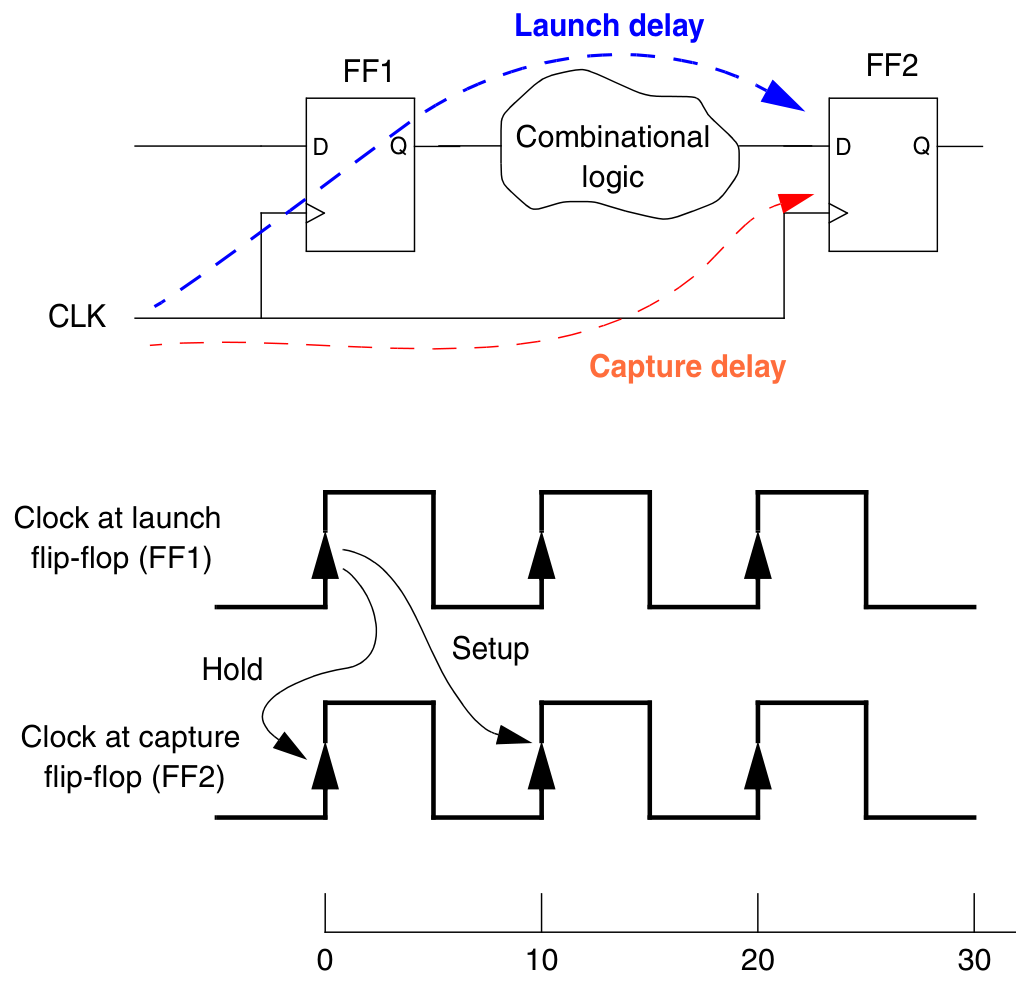
\includegraphics[width=0.9\textwidth]{fig-3-2.png}
  \caption{同一 launch 与 capture 时钟的 setup 与 hold 分析}
  \label{fig:3-2}
\end{figure}

时序分析期间，工具执行：
\begin{itemize}
  \item setup 检查，验证从 FF1 在时刻 0 发射的数据，能否及时到达 FF2 的 D 输入，以满足时刻 10 处 capture 沿的 setup 要求。\\
        若数据到达过晚、不能满足数据 setup 要求，工具报告 setup 违例。
  \item hold 检查，验证从 FF1 在时刻 0 发射的数据不会过早到达 FF2，即不会在 FF2 上一条数据满足 hold 要求之前到达。\\
        若数据到达过早，工具报告 hold 违例。
\end{itemize}

计算 launch 路径与 capture 路径上的延迟时，工具计入时钟网络效应带来的延迟，例如时钟源延迟（source latency）、网络延迟（network latency）以及时钟不确定性（clock uncertainty）。

\section{不同 launch 与 capture 时钟的路径延迟分析}
\subsection*{Path Delay Analysis for Different Launch and Capture Clocks}

对多时钟设计，工具默认假定所有时钟彼此同步，相位关系固定。时序分析时，若路径的 launch 时钟与 capture 时钟不同，工具考虑 launch 时钟沿之后最近的那个可能 capture 时钟沿，并据此确定该路径最紧的 setup 与 hold 要求。

下图给出一条由两个不同时钟分别发射和捕获的路径。

\begin{figure}[htbp]
  \centering
  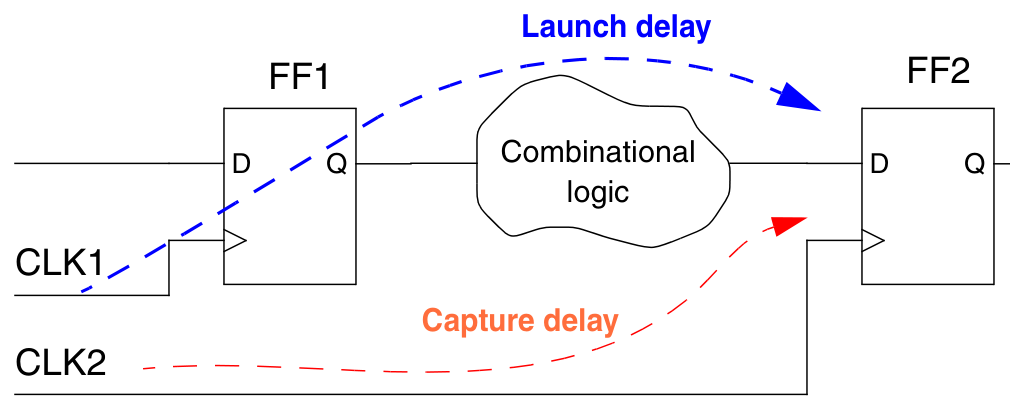
\includegraphics[width=0.9\textwidth]{fig-3-3.png}
  \caption{由不同时钟发射并捕获的路径}
  \label{fig:3-3}
\end{figure}

本例中的时钟 CLK1 与 CLK2 由下列命令创建：
\begin{lstlisting}
icc2_shell> create_clock -period 10 -waveform {0 5} CLK1
icc2_shell> create_clock -period 25 -waveform {5 12.5} CLK2
\end{lstlisting}

\subsection{不同 launch 与 capture 时钟的 setup 分析}
\subsubsection*{Setup Analysis for Different Launch and Capture Clocks}

launch 时钟与 capture 时钟不同时，工具在一段重复周期内考察两者有效沿之间的关系。这段时间长度是两个时钟周期的最小公倍数。对目标触发器的每一个 capture 沿，工具假定对应的 launch 沿是该 capture 沿之前最近的源时钟沿。

在下图中，工具考虑两种 launch 与 capture 沿的组合：
\begin{itemize}
  \item capture 沿在 time = 5，其之前最近的 launch 沿在 time = 0，标为 Setup 1。
  \item capture 沿在 time = 30，其之前最近的 launch 沿在 time = 20，标为 Setup 2。
\end{itemize}

\begin{figure}[htbp]
  \centering
  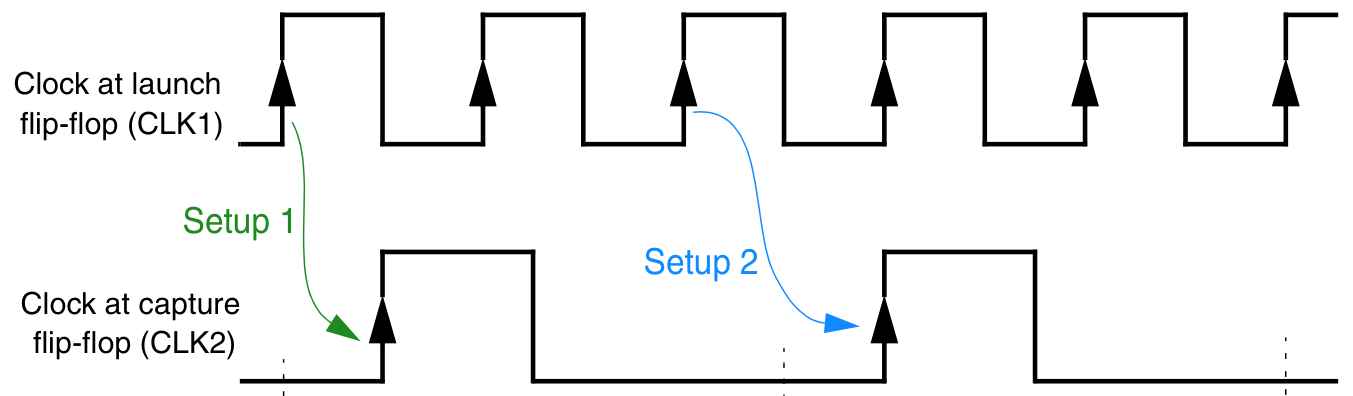
\includegraphics[width=0.9\textwidth]{fig-3-4.png}
  \caption{不同 launch 与 capture 时钟的 setup 分析}
  \label{fig:3-4}
\end{figure}

time = 30 的源时钟沿与 capture 沿同时发生，而不是更早，因此不把它当作对应的 launch 沿。

Setup 1 在 launch 与 capture 之间留出的时间更少，因此是更紧的约束，并决定该路径允许的最大延迟。本例中该值为 5。

\subsection{不同 launch 与 capture 时钟的 hold 分析}
\subsubsection*{Hold Analysis for Different Launch and Capture Clocks}

工具所检查的 hold 关系，基于用来确定 setup 关系的那些时钟沿的相邻沿。为确定最紧的 hold 关系，工具考虑全部有效的 setup 关系，包括下图中的 Setup 1 与 Setup 2。

\begin{figure}[htbp]
  \centering
  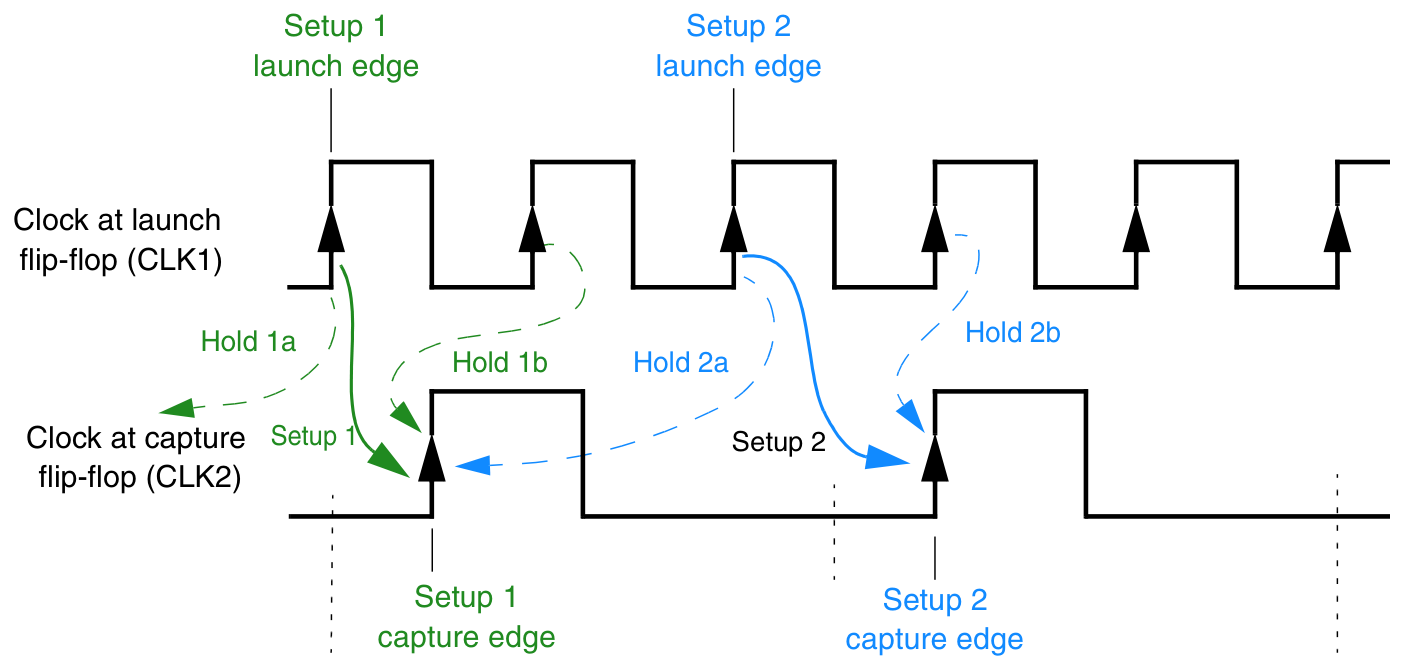
\includegraphics[width=0.9\textwidth]{fig-3-5.png}
  \caption{不同 launch 与 capture 时钟的 hold 分析}
  \label{fig:3-5}
\end{figure}

对每一种 setup 关系，工具做两种不同的 hold 检查：
\begin{itemize}
  \item 由该 setup 的 launch 沿发射的数据，不得被前一个 capture 沿捕获。
  \item 由下一个 launch 沿发射的数据，不得被该 setup 的 capture 沿捕获。
\end{itemize}

对标为 Setup 1 的 setup 关系，对应的两种 hold 检查标为 Hold1a 与 Hold1b。同样，对标为 Setup 2 的 setup 关系，两种 hold 检查标为 Hold2a 与 Hold2b。

在这些 hold 检查中，最紧的是 capture 沿相对 launch 沿发生得最晚的那一次，即 Hold 2b。因此 Hold 2b 决定该路径允许的最小延迟，本例中该值为 0。

\section{输入延迟与输出延迟简介}
\subsection*{Introduction to Input and Output Delays}

要分析一条时序路径，路径的起点和终点都必须受到约束。默认情况下，工具不知道数据到达输入端口的时刻，也不知道输出端口上数据的要求时刻。因此，要约束输入端口与输出端口，必须指定这些信息。

在下图中，到达名为 BlockA 的 block 的输入端口 A 的数据，由外部时序器件发射。

\begin{figure}[htbp]
  \centering
  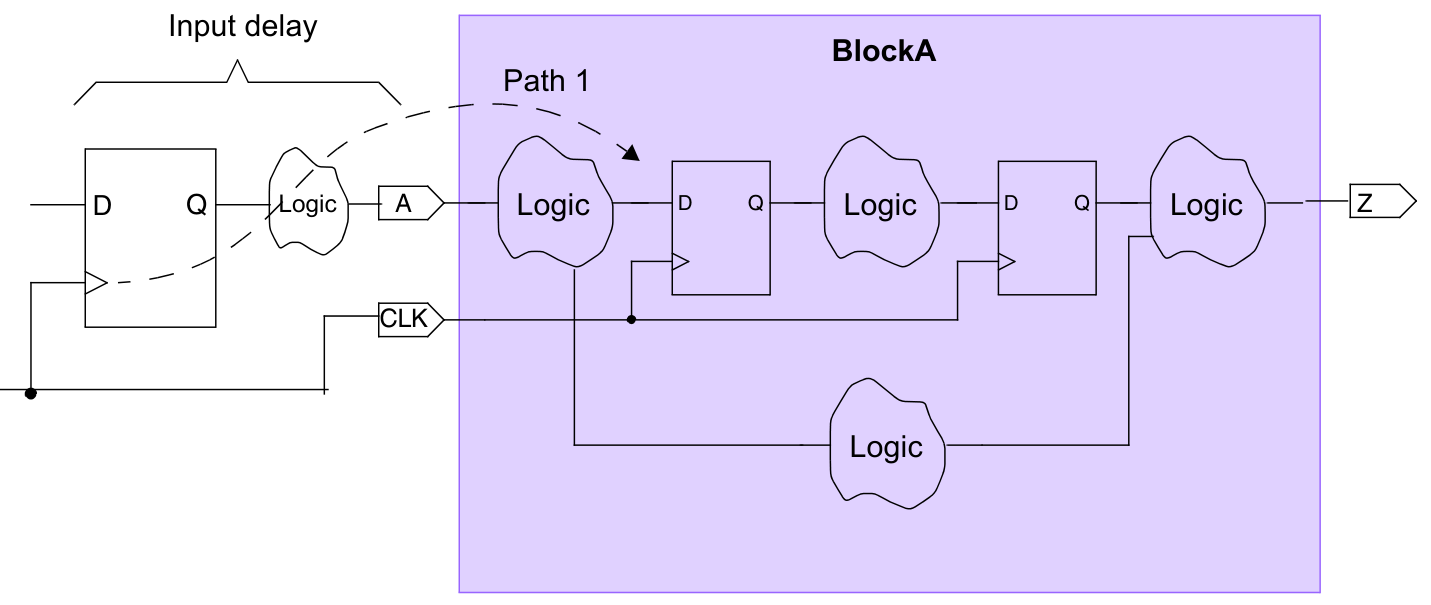
\includegraphics[width=0.9\textwidth]{fig-3-6.png}
  \caption{外部输入延迟}
  \label{fig:3-6}
\end{figure}

要约束输入端口 A，使用 \cmd{set\_input\_delay}，并指定：
\begin{itemize}
  \item 在外部时序器件上发射该数据的时钟。
  \item 数据被发射之后、到达该输入端口之前的延迟。
\end{itemize}

在下图中，离开名为 BlockA 的 block 的输出端口 Z 的数据，由外部时序器件捕获。

\begin{figure}[htbp]
  \centering
  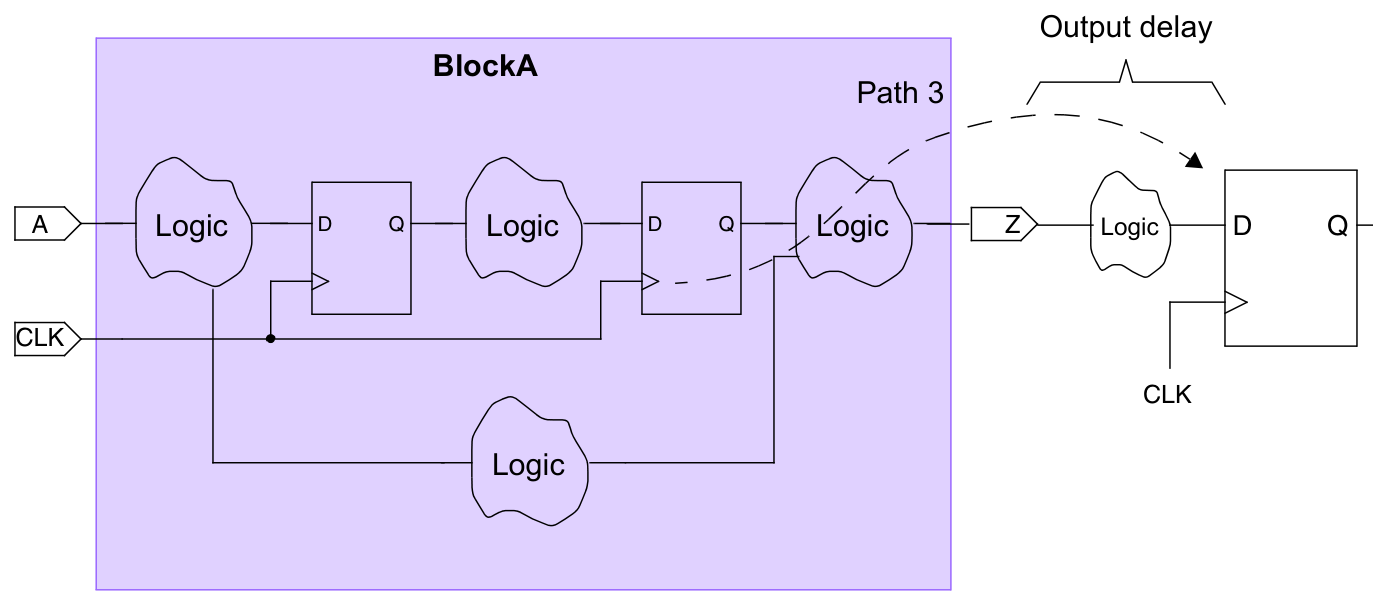
\includegraphics[width=0.9\textwidth]{fig-3-7.png}
  \caption{外部输出延迟}
  \label{fig:3-7}
\end{figure}

要约束输出端口 Z，使用 \cmd{set\_output\_delay}，并指定：
\begin{itemize}
  \item 在外部时序器件上捕获该数据的时钟。
  \item 数据离开端口 Z 之后、到达外部时序器件之前的延迟。
\end{itemize}

\section{为端口设置输入延迟与输出延迟}
\subsection*{Setting Input and Output Delays for Ports}

要靠指定端口外侧的外部延迟来约束输入或输出端口，使用 \cmd{set\_input\_delay} 或 \cmd{set\_output\_delay}。也可以用这两条命令在 block 内部的引脚上施加输入或输出延迟，从而使该引脚成为时序路径的起点或终点。

使用 \cmd{set\_input\_delay} 或 \cmd{set\_output\_delay} 时，必须指定下列信息：
\begin{itemize}
  \item 输入或输出延迟值。
  \item 所约束的端口或引脚。
\end{itemize}

为使时序分析更准确，用下列两种方法之一指定相关时钟：
\begin{itemize}
  \item 用 \opt{-clock} 给出参考时钟的名称。\\
        指定 \opt{-clock} 时，工具默认：
        \begin{itemize}
          \item 假定输入或输出延迟相对于该时钟的上升沿。若延迟相对于下降沿，把 \opt{-clock\_fall} 与 \opt{-clock} 一起使用。
          \item 把为参考时钟指定的 source latency 与 network latency，加到与该输入或输出延迟相关联的 launch 或 capture 路径上。\\
                若参考时钟的 source latency 与 network latency 已经包含在输入或输出延迟之中，使用 \opt{-source\_latency\_included} 与 \opt{-network\_latency\_included}。若参考时钟是 propagated clock，则忽略 \opt{-network\_latency\_included}。
        \end{itemize}
  \item 用 \opt{-reference\_pin} 指定参考时钟网络上的一个引脚或端口。\\
        指定 \opt{-reference\_pin} 时，工具默认：
        \begin{itemize}
          \item 用所有能够到达该参考引脚的时钟来约束端口。要选定某一个时钟，把 \opt{-clock} 与 \opt{-reference\_pin} 一起使用。
          \item 对到达该参考引脚的 ideal clock，把为该时钟指定的 source latency 与 network latency，加到与输入或输出延迟对应的 launch 或 capture 路径上。\\
                对到达该参考引脚的 propagated clock，工具把为该时钟指定的 source delay，以及传播到该参考引脚为止的时钟网络延迟，加到与输入或输出延迟对应的 launch 或 capture 路径上。
        \end{itemize}
\end{itemize}

若不指定相关时钟，工具根据当前 block 的时钟派生一个新时钟。

使用 \cmd{set\_input\_delay} 或 \cmd{set\_output\_delay} 时，可以指定该延迟：
\begin{itemize}
  \item 只用 \opt{-rise} 或 \opt{-fall} 作用于上升或下降跳变。\\
        默认情况下，工具把该延迟同时用于输入或输出端口上的上升与下降跳变。
  \item 只用 \opt{-max} 或 \opt{-min} 作用于最长或最短路径。\\
        默认情况下，工具把该延迟同时用于最长路径与最短路径。
  \item 用 \opt{-level\_sensitive} 相对于电平敏感锁存器。\\
        默认情况下，工具假定与该输入或输出延迟相关联的时序路径，由边沿敏感触发器发射或捕获。
  \item 用 \opt{-add\_delay} 不覆盖已有的输入或输出延迟设置。\\
        用该选项为同一端口相对于不同参考时钟指定不同的输入或输出延迟。
\end{itemize}

对具有多个 scenario 的设计，输入或输出延迟默认只作用于当前 scenario。要为其他范围指定输入或输出延迟：
\begin{itemize}
  \item 特定 mode 的全部 scenario：使用 \opt{-modes}。
  \item 特定 corner 的全部 scenario 以及当前 mode：使用 \opt{-corners}。
  \item 特定 mode 与 corner 的全部 scenario：同时使用 \opt{-modes} 与 \opt{-corners}。
  \item 特定 scenario：使用 \opt{-scenarios}。\\
        使用该选项时，不能同时使用 \opt{-modes} 或 \opt{-corners}。
\end{itemize}

要从端口上去掉输入或输出延迟，使用 \cmd{remove\_input\_delay} 或 \cmd{remove\_output\_delay}。

下图给出一个 block 的一个输入与一个输出的外部路径，以及与这些外部路径相关联的延迟。

\begin{figure}[htbp]
  \centering
  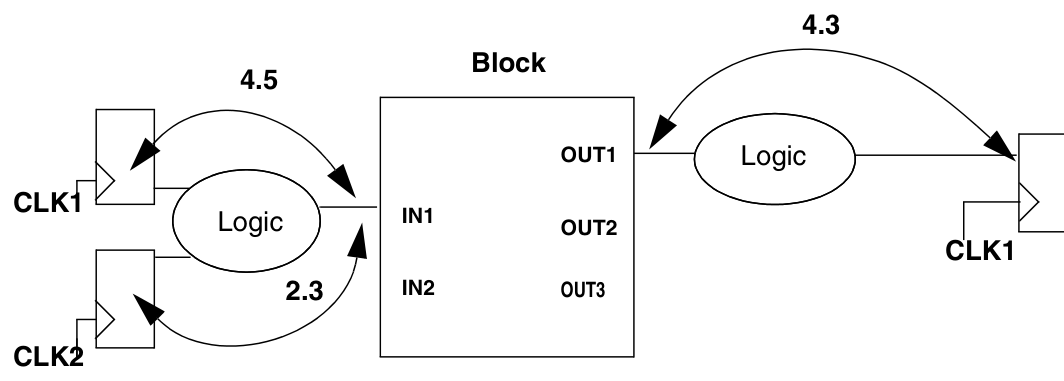
\includegraphics[width=0.9\textwidth]{fig-3-8.png}
  \caption{输入端口与输出端口的外部延迟}
  \label{fig:3-8}
\end{figure}

下列命令约束名为 IN1 的输入：相对于名为 CLK1 的时钟设置输入延迟 4.5，并相对于名为 CLK2 的时钟设置输入延迟 2.3。
\begin{lstlisting}
icc2_shell> set_input_delay 4.5 -clock CLK1 [get_ports IN1]
icc2_shell> set_input_delay 2.3 -clock CLK2 [get_ports IN1] \
 -add_delay
\end{lstlisting}

下列命令约束名为 OUT1 的输出：相对于名为 CLK1 的时钟设置输出延迟 4.3。
\begin{lstlisting}
icc2_shell> set_output_delay 4.3 -clock CLK1 [get_ports OUT1]
\end{lstlisting}

\subsection{考虑 driving cell 延迟的影响}
\subsubsection*{Considering the Effect of Delays Through Driving Cells}

若用 \cmd{set\_driving\_cell} 约束输入或 inout 端口，如下例所示，工具会把外部 driving cell 延迟中随负载变化的那一部分，计入从该端口开始的时序路径，如下图所示。
\begin{lstlisting}
icc2_shell> set_driving_cell -lib_cell AND2 -from_pin A [get_ports I1]
\end{lstlisting}

\begin{figure}[htbp]
  \centering
  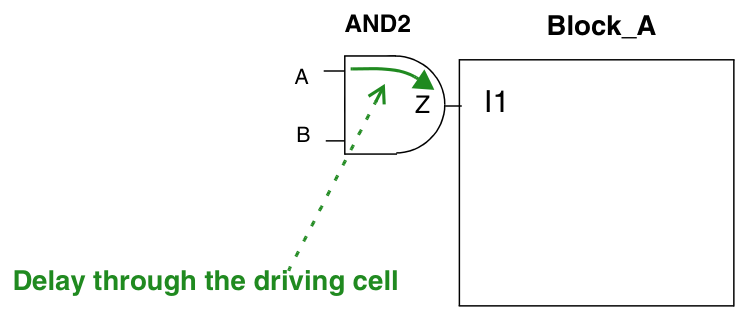
\includegraphics[width=0.9\textwidth]{fig-3-9.png}
  \caption{driving cell 上的延迟}
  \label{fig:3-9}
\end{figure}

为避免这段延迟被计算两次，先估计 driving cell 随负载变化的延迟，再从端口上指定的输入延迟中减去该值。

\subsection{时钟端口上 input delay 的影响}
\subsubsection*{Effect of Input Delay on Clock Ports}

若时钟是 propagated clock，工具把时钟源端口或引脚上的输入延迟当作 source latency。该输入延迟可以不相对于任何时钟，也可以相对于该源自身的时钟。source latency 值会加到时钟网络延迟上，得到总延迟（total latency）。

不要像下例这样对全部输入端口设置输入延迟：
\begin{lstlisting}
icc2_shell> set_input_delay 2 -clock CLK [all_inputs]
\end{lstlisting}

应当对除时钟端口以外的全部输入设置输入延迟，如下例所示：
\begin{lstlisting}
icc2_shell> set_input_delay 2 -clock CLK \
       [remove_from_collection [all_inputs] [get_ports CLK]]
\end{lstlisting}

若存在实际的 source latency，用带 \opt{-source} 的 \cmd{set\_clock\_latency} 来定义。

\section{指定时序例外}
\subsection*{Specifying Timing Exceptions}

IC Compiler II 允许设置下列类型的时序例外：
\begin{itemize}
  \item false path：标出不需要做时序分析的路径。\\
        使用 \cmd{set\_false\_path}，见“指定 false path 例外”。
  \item 最小与最大延迟值：在指定起点与终点之间设置最小与最大路径延迟要求。\\
        使用 \cmd{set\_max\_delay} 与 \cmd{set\_min\_delay}，见“指定最大与最小路径延迟例外”。
  \item multicycle path：用指定路径所需的时钟周期数，覆盖默认的单周期要求。\\
        使用 \cmd{set\_multicycle\_path}，见“指定 multicycle path 例外”。
  \item 路径时序裕量（path timing margin）：按指定的时间量收紧或放宽指定路径的时序要求。\\
        使用 \cmd{set\_path\_margin}，见“指定路径时序裕量例外”。
\end{itemize}

每条时序例外命令既可以作用于单条路径，也可以作用于一组相关路径，例如从一个时钟域到另一个时钟域的全部路径，或经过设计中某指定点的全部路径。

要报告已经施加到设计上的全部时序例外，使用 \cmd{report\_exceptions}。

要把路径恢复到施加时序例外之前的默认状态，使用 \cmd{reset\_paths}，或使用各时序例外命令的 \opt{-reset\_path} 选项。

\section{指定 false path 例外}
\subsection*{Specifying False Path Exceptions}

false path 是不需要做时序分析的路径。例如，两个经多路选择的逻辑块之间可以存在一条路径，但两者从不同时被选中，因此该路径对时序分析无效。把这类路径指定为 false path，可避免工具把时间花在分析真实设计中不会出现的时序路径上。

要用 \cmd{set\_false\_path} 把时序路径定义为 false path，必须用下列一种或多种方法指定要设置的路径：
\begin{itemize}
  \item 用 \opt{-from}、\opt{-rise\_from} 或 \opt{-fall\_from} 指定路径起点。\\
        有效起点为：
        \begin{itemize}
          \item 时钟。\\
                若指定时钟，则从该时钟所约束的全部时序单元与原始端口出发的时序路径都被设为 false path。
          \item 时序单元。
          \item 时序单元的时钟引脚。
          \item 锁存器的数据引脚。
          \item 输入或 inout 端口。
          \item 已设置 input delay 的引脚。
        \end{itemize}
  \item 用 \opt{-through}、\opt{-rise\_through} 或 \opt{-fall\_through} 指定一个或多个经过点，这些选项可使用一次或多次。\\
        有效经过点为：
        \begin{itemize}
          \item 引脚
          \item 端口
          \item 单元
          \item 线网
        \end{itemize}
        若经过某引脚的全部路径都是 false path，用 \cmd{set\_disable\_timing} 禁用该引脚的时序弧，比使用 \cmd{set\_false\_path} \opt{-through} 更高效。
  \item 用 \opt{-to}、\opt{-rise\_to} 或 \opt{-fall\_to} 指定路径终点。\\
        有效终点为：
        \begin{itemize}
          \item 时钟。\\
                若指定时钟，则结束于该时钟所约束的全部时序单元与原始端口的时序路径都被设为 false path。
          \item 时序单元。
          \item 时序单元的数据引脚。
          \item 输出或 inout 端口。
          \item 已设置 output delay 的引脚。
        \end{itemize}
\end{itemize}

可选地，可以把 false path 设置限制为：
\begin{itemize}
  \item 只用 \opt{-setup} 或 \opt{-hold} 作用于 setup 或 hold 分析。\\
        默认情况下，false path 设置同时作用于 setup 与 hold 分析。
  \item 只用 \opt{-rise} 或 \opt{-fall} 作用于上升或下降分析。\\
        默认情况下，false path 设置同时作用于上升与下降分析。
\end{itemize}

要去掉 false path 设置，使用 \cmd{set\_false\_path} \opt{-reset\_path} 或 \cmd{reset\_paths}。

下例把一条很具体的路径设为 false path：从寄存器时钟引脚出发，经过若干引脚，结束于寄存器数据引脚。
\begin{lstlisting}
icc2_shell> set_false_path -from [get_pins reg2/CP] \
  -through [get_pins U31/Z] -through [get_pins U15/Z] \
  -to [get_pins reg7/D]
\end{lstlisting}

下例把时钟 ck1 与 ck2 之间的全部时序路径设为 false path：
\begin{lstlisting}
icc2_shell> set_false_path -from [get_clocks ck1] \
          -to [get_clocks ck2]
icc2_shell> set_false_path -from [get_clocks ck2] \
          -to [get_clocks ck1]
\end{lstlisting}

对本例，另一种做法是用 \cmd{set\_clock\_groups} 把时钟 ck1 与 ck2 之间的全部路径排除在时序分析之外。

\section{指定最大与最小路径延迟例外}
\subsection*{Specifying Maximum and Minimum Path Delay Exceptions}

默认情况下，工具根据 launch 与 capture 时钟沿的时刻计算路径允许的最大与最小延迟。要用自己的具体延迟约束覆盖默认的最大或最小允许路径延迟，使用 \cmd{set\_max\_delay} 或 \cmd{set\_min\_delay}。也可以用这两条命令约束一条不受时钟约束的纯组合时序路径。

使用 \cmd{set\_max\_delay} 或 \cmd{set\_min\_delay} 时，必须指定：
\begin{itemize}
  \item 最大或最小延迟值。
  \item 要用下列一种或多种方法约束的路径：
        \begin{itemize}
          \item 用 \opt{-from}、\opt{-rise\_from} 或 \opt{-fall\_from} 指定路径起点。\\
                有效起点为：
                \begin{itemize}
                  \item 时钟。\\
                        若指定时钟，则从该时钟所约束的全部时序单元与原始端口出发的时序路径都施加该最大或最小延迟。
                  \item 时序单元。
                  \item 时序单元的时钟引脚。
                  \item 锁存器的数据引脚。
                  \item 输入或 inout 端口。
                  \item 已设置 input delay 的引脚。
                \end{itemize}
          \item 用 \opt{-through}、\opt{-rise\_through} 或 \opt{-fall\_through} 指定一个或多个经过点，这些选项可使用一次或多次。\\
                有效经过点为：
                \begin{itemize}
                  \item 引脚
                  \item 端口
                  \item 单元
                  \item 线网
                \end{itemize}
          \item 用 \opt{-to}、\opt{-rise\_to} 或 \opt{-fall\_to} 指定路径终点。\\
                有效终点为：
                \begin{itemize}
                  \item 时钟。\\
                        若指定时钟，则结束于该时钟所约束的全部时序单元与原始端口的时序路径都施加该最大或最小延迟。
                  \item 时序单元。
                  \item 时序单元的数据引脚。
                  \item 输出或 inout 端口。
                  \item 已设置 output delay 的引脚。
                \end{itemize}
        \end{itemize}
\end{itemize}

可选地，可以把最大或最小路径延迟设置限制为：
\begin{itemize}
  \item 只用 \opt{-setup} 或 \opt{-hold} 作用于 setup 或 hold 分析。\\
        默认情况下，它同时作用于 setup 与 hold 分析。
  \item 只用 \opt{-rise} 或 \opt{-fall} 作用于上升或下降分析。\\
        默认情况下，它同时作用于上升与下降分析。
\end{itemize}

若施加 \cmd{set\_max\_delay} 或 \cmd{set\_min\_delay} 的路径起点或终点受时钟约束，时序分析时工具会使用起点与终点的时钟延迟。要忽略起点与终点的时钟延迟，使用 \opt{-ignore\_clock\_latency}。

要去掉最大或最小路径延迟设置，使用 \cmd{set\_max\_delay} 或 \cmd{set\_min\_delay} 的 \opt{-reset\_path} 选项，或使用 \cmd{reset\_paths}。

下例把寄存器 REGA 与 REGB 之间的最大路径延迟设为 12，最小路径延迟设为 2：
\begin{lstlisting}
icc2_shell> set_max_delay 12.0 \
          -from [get_cells REGA] -to [get_cells REGB]
icc2_shell> set_min_delay 2.0 \
          -from [get_cells REGA] -to [get_cells REGB]
\end{lstlisting}

\section{指定 multicycle path 例外}
\subsection*{Specifying Multicycle Path Exceptions}

若数据从路径起点传播到终点所需的时钟周期数，多于工具使用的单周期要求，可以用 \cmd{set\_multicycle\_path} 为该路径指定额外的时钟周期。随后工具按指定的周期数计算 setup 或 hold 约束。

使用 \cmd{set\_multicycle\_path} 时，必须指定：
\begin{itemize}
  \item 要为该路径分配的时钟周期数。\\
        若路径的 launch 时钟与 capture 时钟不是同一个时钟，用 \opt{-start} 或 \opt{-end} 说明周期数基于 launch 时钟还是 capture 时钟。默认情况下，工具相对于 capture 时钟移动 setup 检查，相对于 launch 时钟移动 hold 检查。
  \item 要用下列一种或多种方法约束的路径：
        \begin{itemize}
          \item 用 \opt{-from}、\opt{-rise\_from} 或 \opt{-fall\_from} 指定路径起点。\\
                有效起点为：
                \begin{itemize}
                  \item 时钟。\\
                        若指定时钟，则从该时钟所约束的全部时序单元与原始端口出发的时序路径都施加该多周期设置。
                  \item 时序单元。
                  \item 时序单元的时钟引脚。
                  \item 锁存器的数据引脚。
                  \item 输入或 inout 端口。
                  \item 已设置 input delay 的引脚。
                \end{itemize}
          \item 用 \opt{-through}、\opt{-rise\_through} 或 \opt{-fall\_through} 指定一个或多个经过点，这些选项可使用一次或多次。\\
                有效经过点为：
                \begin{itemize}
                  \item 引脚
                  \item 端口
                  \item 单元
                  \item 线网
                \end{itemize}
          \item 用 \opt{-to}、\opt{-rise\_to} 或 \opt{-fall\_to} 指定路径终点。\\
                有效终点为：
                \begin{itemize}
                  \item 时钟。\\
                        若指定时钟，则结束于该时钟所约束的全部时序单元与原始端口的时序路径都施加该多周期设置。
                  \item 时序单元。
                  \item 时序单元的数据引脚。
                  \item 输出或 inout 端口。
                  \item 已设置 output delay 的引脚。
                \end{itemize}
        \end{itemize}
\end{itemize}

可选地，可以把 multicycle path 设置限制为：
\begin{itemize}
  \item 只用 \opt{-setup} 或 \opt{-hold} 作用于 setup 或 hold 分析。\\
        默认情况下，它同时作用于 setup 与 hold 分析。\\
        工具对 \cmd{set\_multicycle\_path} 中 \opt{-setup} 与 \opt{-hold} 的数值解释不同。\opt{-setup} 参数的整数值指定 multicycle path 的时钟周期数。没有时序例外时，默认值为 1。\opt{-hold} 参数的整数值指定：相对于有效 setup 关系，把 capture 沿从默认位置向后移动的时钟周期数。默认值为 0。
  \item 只用 \opt{-rise} 或 \opt{-fall} 作用于上升或下降分析。\\
        默认情况下，它同时作用于上升与下降分析。
\end{itemize}

要去掉 multicycle path 设置，使用 \cmd{set\_multicycle\_path} \opt{-reset\_path} 或 \cmd{reset\_paths}。

\subsection{为 hold 分析指定正确的周期数}
\subsubsection*{Specifying the Correct Number of Multicycles for Hold Analysis}

下面的例子说明：当已经知道 setup 分析所需的周期数时，如何确定 hold 分析所需的正确周期数。

本例中，名为 Reg4 与 Reg5 的寄存器之间的时序路径按两个时钟周期设计。默认情况下，工具对所有路径都按单周期时序处理。因此需要用下列命令为这条路径指定时序例外。

要为该 block 设置 multicycle path，使用下列命令：
\begin{lstlisting}
icc2_shell> set_multicycle_path -setup 2 \
          -from [get_cells Reg4] -to [get_cells Reg5]
\end{lstlisting}

该命令指定这条路径占用两个时钟周期，并建立下图所示的新 setup 关系。launch 沿之后的第二个 capture 沿，成为路径终点所适用的沿。

\begin{figure}[htbp]
  \centering
  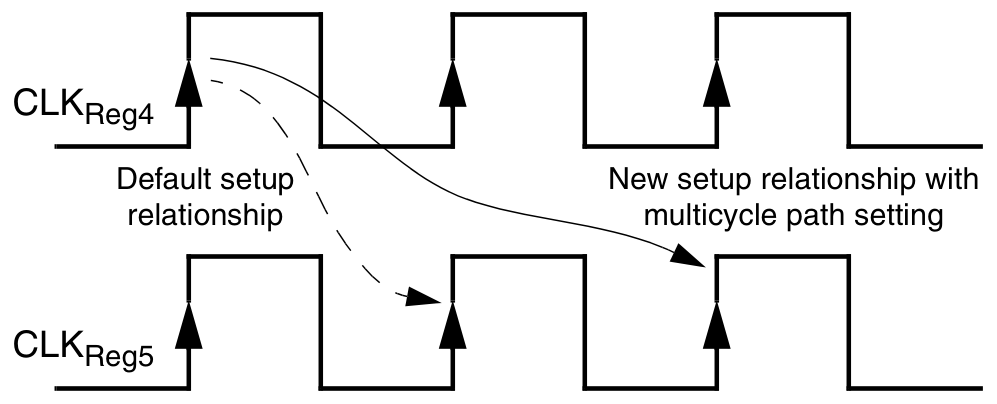
\includegraphics[width=0.9\textwidth]{fig-3-10.png}
  \caption{多周期路径的 setup}
  \label{fig:3-10}
\end{figure}

改变 setup 关系也会隐含地改变 hold 关系，因为所有 hold 关系都基于有效的 setup 关系。工具验证：由 setup 的 launch 沿发射的数据，不会被前一个 capture 沿捕获。新的 hold 关系如下图所示。

\begin{figure}[htbp]
  \centering
  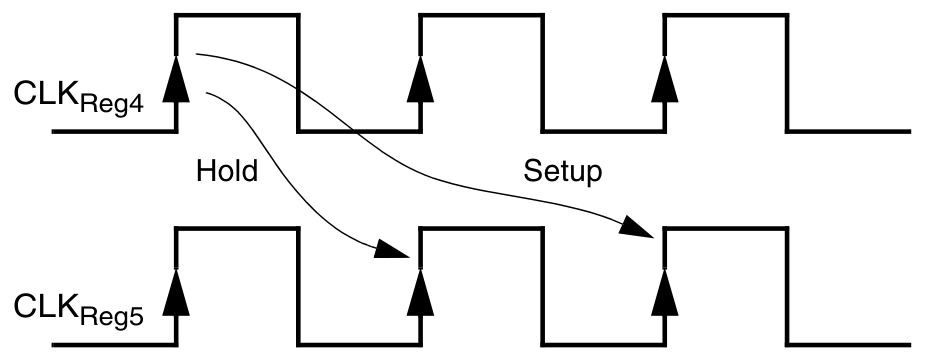
\includegraphics[width=0.9\textwidth]{fig-3-11.png}
  \caption{基于新 setup 关系的多周期路径 hold}
  \label{fig:3-11}
\end{figure}

图中所示的 hold 关系多半不是该设计的正确关系。若 Reg4 不需要把数据保持到第一个时钟沿之后，就必须指定 multicycle hold 时序例外，命令如下：
\begin{lstlisting}
icc2_shell> set_multicycle_path -setup 2 \
          -from [get_cells Reg4] -to [get_cells Reg5]
icc2_shell> set_multicycle_path -hold 1 \
          -from [get_cells Reg4] -to [get_cells Reg5]
\end{lstlisting}

下图给出用这两条 \cmd{set\_multicycle\_path} 正确设置后的 setup 与 hold 关系。第二条 \cmd{set\_multicycle\_path} 把 hold 关系的 capture 沿向后移动一个时钟周期，从虚线箭头移到实线箭头。

\begin{figure}[htbp]
  \centering
  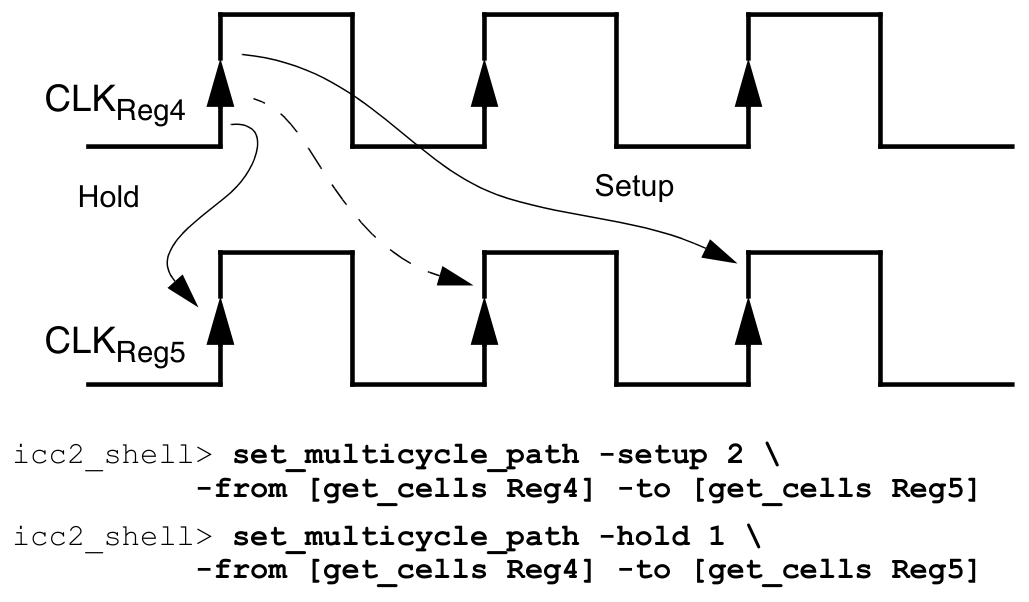
\includegraphics[width=0.9\textwidth]{fig-3-12.png}
  \caption{正确设置的多周期路径 hold}
  \label{fig:3-12}
\end{figure}

工具按下列公式确定 hold 周期数：

\begin{center}
\texttt{(hold cycles) = (setup option value) - 1 - (hold option value)}
\end{center}

默认情况下，hold cycles = 1 - 1 - 0 = 0。本例中 hold cycles = 2 - 1 - 1 = 0，这给出默认的 hold 行为。

\section{指定路径时序裕量例外}
\subsection*{Specifying Path Timing Margin Exceptions}

可以用 \cmd{set\_path\_margin} 使指定路径的时序检查按给定的时间量变得更松或更紧。

使用 \cmd{set\_path\_margin} 时，必须指定：
\begin{itemize}
  \item 裕量值。\\
        正值使检查更紧（more restrictive）。负值使检查更松（less restrictive）。
  \item 要用下列一种或多种方法约束的路径：
        \begin{itemize}
          \item 用 \opt{-from}、\opt{-rise\_from} 或 \opt{-fall\_from} 指定路径起点。\\
                有效起点为：
                \begin{itemize}
                  \item 时钟。\\
                        若指定时钟，则从该时钟所约束的全部时序单元与原始端口出发的时序路径都施加该路径裕量。
                  \item 时序单元。
                  \item 时序单元的时钟引脚。
                  \item 锁存器的数据引脚。
                  \item 输入或 inout 端口。
                  \item 已设置 input delay 的引脚。
                \end{itemize}
          \item 用 \opt{-through}、\opt{-rise\_through} 或 \opt{-fall\_through} 指定一个或多个经过点，这些选项可使用一次或多次。\\
                有效经过点为：
                \begin{itemize}
                  \item 引脚
                  \item 端口
                  \item 单元
                  \item 线网
                \end{itemize}
          \item 用 \opt{-to}、\opt{-rise\_to} 或 \opt{-fall\_to} 指定路径终点。\\
                有效终点为：
                \begin{itemize}
                  \item 时钟。\\
                        若指定时钟，则结束于该时钟所约束的全部时序单元与原始端口的时序路径都施加该路径裕量。
                  \item 时序单元。
                  \item 时序单元的数据引脚。
                  \item 输出或 inout 端口。
                  \item 已设置 output delay 的引脚。
                \end{itemize}
        \end{itemize}
\end{itemize}

可选地，可以把路径裕量设置限制为：
\begin{itemize}
  \item 只用 \opt{-setup} 或 \opt{-hold} 作用于 setup 或 hold 分析。\\
        默认情况下，它同时作用于 setup 与 hold 分析。
  \item 只用 \opt{-rise} 或 \opt{-fall} 作用于上升或下降分析。\\
        默认情况下，它同时作用于上升与下降分析。
\end{itemize}

要去掉路径裕量设置，使用 \cmd{set\_path\_margin} \opt{-reset\_path}。

下例使从单元 Reg4 到单元 Reg5 的全部 setup 检查收紧 1.2 个时间单位。
\begin{lstlisting}
icc2_shell> set_path_margin 1.2 \
   -from [get_cells Reg4] -to [get_cells Reg5]
\end{lstlisting}

所指定的裕量是在同一路径上已有的 minimum-delay、maximum-delay 与 multicycle path 例外之外，再叠加到时序检查上。施加在同一路径上的 false path 例外优先于路径时序裕量例外，裕量设置因此被忽略。

\section{高效地指定例外}
\subsection*{Specifying Exceptions Efficiently}

很多情况下，例外路径可以用许多不同方式指定。为缩短时序分析的运行时间，指定例外时遵循下列准则：
\begin{itemize}
  \item 先看清使例外成为必要的根本原因，再为受影响的路径找到控制时序分析的最简单方法。
  \item 在使用 false path 之前，考虑：
        \begin{itemize}
          \item 用 \cmd{set\_case\_analysis} 设置 case analysis。
          \item 用 \cmd{set\_clock\_groups} 声明时钟之间的互斥关系。
          \item 用 \cmd{set\_disable\_timing} 禁用设计中某一部分的分析。
        \end{itemize}
        这些替代方法可以比 \cmd{set\_false\_path} 更高效。
  \item 若必须设置 false path，避免用 \opt{-through} 或通配符指定大量路径。
\end{itemize}

例如，考虑下图所示电路。三个 16 位寄存器分别由三个不同时钟打拍。每个寄存器代表 16 个触发器。寄存器 REG2 只用于测试，因此电路正常工作时，从 REG2 到 REG3 的全部路径都是 false path。

\begin{figure}[htbp]
  \centering
  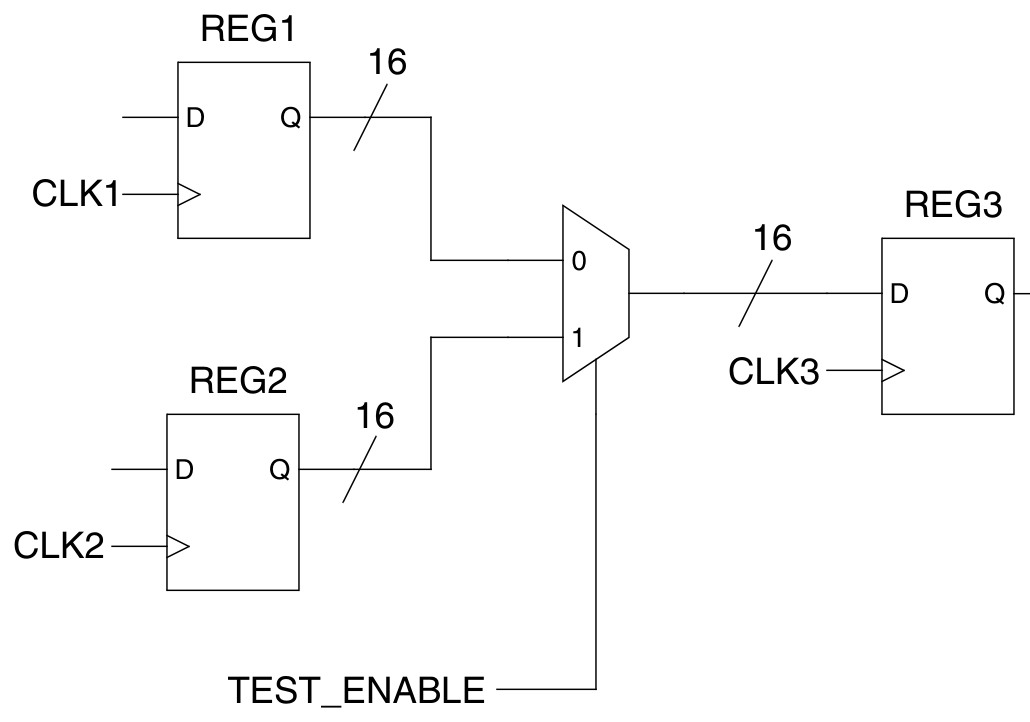
\includegraphics[width=0.9\textwidth]{fig-3-13.png}
  \caption{经过多路选择的寄存器路径}
  \label{fig:3-13}
\end{figure}

要忽略从 REG2 到 REG3 的时序，可以使用下列任一方法：
\begin{itemize}
  \item 用 case analysis 考虑测试使能信号为 0 的情形。
  \item 在 CLK1 与 CLK2 时钟域之间设置互斥关系。
  \item 把时钟域 CLK2 与 CLK3 之间的路径声明为 false。
\begin{lstlisting}
icc2_shell> set_false_path \
          -from [get_clocks CLK2] -to [get_clocks CLK3]
\end{lstlisting}
        这种方法指定 false path 的效率较高，因为工具只需要记录所指定的时钟域，不必记录寄存器、引脚、线网等对象上的例外。
  \item 把从 REG2 到 REG3 的 16 条单独路径声明为 false。
\begin{lstlisting}
icc2_shell> set_false_path -from [get_pins REG2[0]/CP] \
          -to [get_pins REG3[0]/D]
icc2_shell> set_false_path -from [get_pins REG2[1]/CP] \
          -to [get_pins REG3[1]/D]
icc2_shell> ...
\end{lstlisting}
        这种方法效率较低，因为工具必须记录 16 条不同路径上的时序例外。
  \item 把从 REG2 到 REG3 的全部路径声明为 false。
\begin{lstlisting}
icc2_shell> set_false_path -from [get_pins REG2[*]/CP] \
          -to [get_pins REG3[*]/D]
\end{lstlisting}
        这种方法效率更低，因为工具必须记录从 REG2 的每个时钟引脚到 REG3 的每个数据引脚的路径，共 256 条。
  \item 把从 REG2 出发的全部路径声明为 false。
\begin{lstlisting}
icc2_shell> set_false_path -from [get_pins REG2[*]/CP]
\end{lstlisting}
        这种方法与前一种类似。工具必须记录从 REG2 每个时钟引脚出发的全部路径，共 256 条。
\end{itemize}

\section{例外的优先级}
\subsection*{Order of Precedence for Exceptions}

对给定 block 中的每一条时序路径，工具找出适用于该路径的全部时序例外。若某条路径适用多个时序例外，实际用于该路径的例外取决于：
\begin{itemize}
  \item 所指定的例外类型，见“按例外类型的优先级”。
  \item 设置例外时使用的路径指定方法，见“按路径指定方式的优先级”。
\end{itemize}

\subsection{按例外类型的优先级}
\subsubsection*{Precedence Based on Exception Type}

下列几对时序例外类型不视为冲突，因此两种设置对一条路径都可以有效：
\begin{itemize}
  \item 两个 \cmd{set\_false\_path} 设置。
  \item \cmd{set\_min\_delay} 与 \cmd{set\_max\_delay} 设置。
  \item \cmd{set\_multicycle\_path} 的 \opt{-setup} 与 \opt{-hold} 设置。
  \item \cmd{set\_path\_margin} 与 \cmd{set\_min\_delay}、\cmd{set\_max\_delay} 或 \cmd{set\_multicycle\_path} 设置。
\end{itemize}

发生冲突时，时序例外类型按下列优先级从高到低排列：
\begin{enumerate}
  \item \cmd{set\_false\_path} 设置
  \item \cmd{set\_max\_delay} 与 \cmd{set\_min\_delay} 设置
  \item \cmd{set\_multicycle\_path} 设置
\end{enumerate}

例如，若把一条路径声明为 false，同时又把它的最大延迟设为某个值，则 false path 声明优先，最大延迟设置被忽略。

\subsection{按路径指定方式的优先级}
\subsubsection*{Precedence Based on Path Specification}

施加在更具体对象（例如引脚或端口）上的时序例外，优先于施加在更一般对象（例如时钟）上的同类例外。

各种路径指定方法按下列优先级从高到低排列：
\begin{enumerate}
  \item \opt{-from} pin、\opt{-rise\_from} pin、\opt{-fall\_from} pin 设置
  \item \opt{-to} pin、\opt{-rise\_to} pin、\opt{-fall\_to} pin 设置
  \item \opt{-through}、\opt{-rise\_through}、\opt{-fall\_through} 设置
  \item \opt{-from} clock、\opt{-rise\_from} clock、\opt{-fall\_from} clock 设置
  \item \opt{-to} clock、\opt{-rise\_to} clock、\opt{-fall\_to} clock 设置
\end{enumerate}

按上述优先级规则，若干可能的路径指定组合从高到低如下：
\begin{enumerate}
  \item \opt{-from} pin \opt{-to} pin
  \item \opt{-from} pin \opt{-to} clock
  \item \opt{-from} pin
  \item \opt{-from} clock \opt{-to} pin
  \item \opt{-to} pin
  \item \opt{-from} clock \opt{-to} clock
  \item \opt{-from} clock
  \item \opt{-to} clock
\end{enumerate}

例如，假定设置了下列例外：
\begin{lstlisting}
icc2_shell> set_max_delay 12 -from [get_clocks CLK1]
icc2_shell> set_max_delay 15 -from [get_clocks CLK1] -to [get_clocks CLK2]
\end{lstlisting}

第一条命令设置从 CLK1 出发的全部路径的最大延迟。第二条命令更具体，因此对从 CLK1 出发并结束于 CLK2 的路径，它覆盖第一条命令。

\subsection{例外优先级示例}
\subsubsection*{Example on the Order of Precedence of Exceptions}

假定一个具有四个时钟 clkA、clkB、clkC 与 clkD 的 block 上有下列例外设置：
\begin{lstlisting}
icc2_shell> set_false_path \
          -from [get_clocks clkB] -to [get_clocks clkC]
icc2_shell> set_multicycle_path  2 \
          -from [get_clocks clkA] -to [get_clocks clkC]
icc2_shell> set_multicycle_path 3 -to [get_pins Reg53/D]
icc2_shell> set_multicycle_path 3 -from [get_pins Reg24/CK]
\end{lstlisting}

对一条从单元 Reg24 出发、结束于单元 Reg32 的时序路径，Reg24 由时钟 clkB 打拍，Reg32 由时钟 clkD 打拍，只有下列例外适用：
\begin{lstlisting}
icc2_shell> set_multicycle_path 3 -from [get_pins Reg24/CK]
\end{lstlisting}

对一条从单元 Reg24 出发、结束于单元 Reg11 的时序路径，Reg24 由时钟 clkB 打拍，Reg11 由时钟 clkC 打拍，下列两个例外都适用：
\begin{lstlisting}
icc2_shell> set_false_path \
          -from [get_clocks clkB] -to [get_clocks clkC]
icc2_shell> set_multicycle_path 3 -from [get_pins Reg24/CK]
\end{lstlisting}

此时 \cmd{set\_false\_path} 优先于 \cmd{set\_multicycle\_path}，因此工具对该路径使用 false path 例外。

对一条从单元 Reg61 出发、结束于单元 Reg53 的时序路径，Reg61 由时钟 clkA 打拍，Reg53 由时钟 clkC 打拍，下列两个例外都适用：
\begin{lstlisting}
icc2_shell> set_multicycle_path  2 \
          -from [get_clocks clkA] -to [get_clocks clkC]
icc2_shell> set_multicycle_path 3 -to [get_pins Reg53/D]
\end{lstlisting}

此时有两条路径指定方式不同的 \cmd{set\_multicycle\_path}，工具采用更具体的路径指定，即到单元 Reg53 的 D 引脚的 multicycle path 设置。

\section{禁用下层 block 内部的时序路径}
\subsection*{Disabling Timing Paths Within Lower-Level Blocks}

对带层次的设计，可以用 \cmd{set\_timing\_paths\_disabled\_blocks} 禁用完全位于下层 block 内部的时序路径，使其不参与时序分析与优化。

要禁用完全位于下列范围之内的时序路径：
\begin{itemize}
  \item 指定的子 block：使用 \opt{-blocks}。
  \item 全部子 block：使用 \opt{-all\_sub\_blocks}。
\end{itemize}

要恢复子 block 内被禁用的时序路径，使用 \cmd{remove\_timing\_paths\_disabled\_blocks}。

\section{使用 case analysis}
\subsection*{Using Case Analysis}

case analysis 让你在端口或引脚上使用逻辑常量或逻辑跳变做时序分析，从而限制在设计中传播的信号。

若 case analysis 设置为：
\begin{itemize}
  \item 逻辑常量，工具禁用该常量所传播到的路径。\\
        使用 \cmd{set\_case\_analysis 0} 或 \cmd{set\_case\_analysis 1}，如下例所示：
\begin{lstlisting}
icc2_shell> set_case_analysis 0 [get_ports TEST_EN]
\end{lstlisting}
  \item 逻辑跳变，上升或下降，工具通过限制分析时所考虑的跳变来消除某些路径。\\
        使用 \cmd{set\_case\_analysis rising} 或 \cmd{set\_case\_analysis falling}，如下例所示：
\begin{lstlisting}
icc2_shell> set_case_analysis rising [get_ports RESET]
\end{lstlisting}
\end{itemize}

此外，工具还把下列情形也当作 case analysis 值：
\begin{itemize}
  \item 连接到 tie-high 或 tie-low 单元的单元引脚。
  \item 未连接的单元引脚，工具把它们接到常量值。
\end{itemize}

可以用下列命令或应用选项设置控制 case analysis：
\begin{itemize}
  \item 把 \appopt{time.case\_analysis\_propagate\_through\_icg} 设为 \cmd{true}，使 case analysis 值穿过时钟门控单元继续传播。\\
        默认情况下，工具在时钟门控单元处停止传播 case analysis 值。
  \item 把 \appopt{time.case\_analysis\_sequential\_propagation} 设为 \cmd{always}，使 case analysis 值穿过时序单元继续传播。\\
        默认情况下，该应用选项为 \cmd{never}，工具在时序单元处停止传播 case analysis 值。
  \item 把 \appopt{time.disable\_case\_analysis\_ti\_hi\_lo} 设为 \cmd{true}，除用 \cmd{set\_case\_analysis} 设置的逻辑常量外，禁止传播其他逻辑常量。\\
        默认情况下，工具传播全部逻辑常量。
  \item 把 \appopt{time.disable\_case\_analysis} 设为 \cmd{true}，禁止传播全部 case analysis 值。\\
        默认情况下，工具传播全部 case analysis 值。
  \item 用 \cmd{remove\_case\_analysis} 去掉指定的 case analysis 值。
\end{itemize}

报告时：
\begin{itemize}
  \item case analysis 值：使用 \cmd{report\_case\_analysis}。
  \item 因各种原因（包括 case analysis）被禁用的时序弧：使用 \cmd{report\_disable\_timing}。
\end{itemize}

下例在名为 TEST\_EN 的输入端口上把 case analysis 设为 0，从而禁用经过图~\ref{fig:3-14} 中名为 U15 的多路选择器的引脚 B 与 Z 的时序路径：
\begin{lstlisting}
icc2_shell> set_case_analysis 0 [get_ports TEST_EN]
\end{lstlisting}

\begin{figure}[htbp]
  \centering
  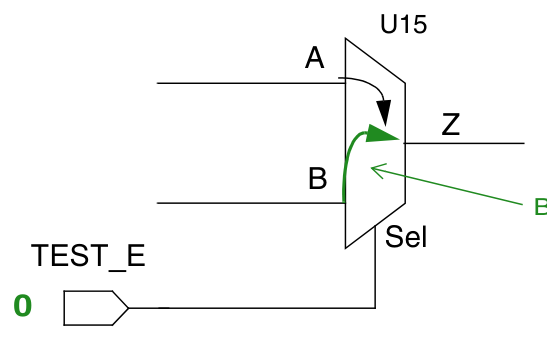
\includegraphics[width=0.9\textwidth]{fig-3-14.png}
  \caption{用常量禁用时序弧}
  \label{fig:3-14}
\end{figure}

\section{禁用时序弧}
\subsection*{Disabling Timing Arcs}

可以用 \cmd{set\_disable\_timing} 禁用路径上的线网或单元时序弧，从而禁用一条时序路径。可以禁用：
\begin{itemize}
  \item 叶级单元或库单元的时序弧。\\
        此时默认禁用到该单元输出的全部时序弧。要禁用单元的某一条时序弧，使用 \opt{-to} 与 \opt{-from}。\\
        例如，下列命令禁用名为 AND3 的库单元到其输出的全部时序弧，以及名为 U17 的单元实例上从引脚 A2 到引脚 ZN 的时序弧：
\begin{lstlisting}
icc2_shell> set_disable_timing my_lib/AND3
icc2_shell> set_disable_timing {U17} -from A2 -to ZN
\end{lstlisting}
  \item 叶级单元引脚、库单元引脚或端口的时序弧。\\
        此时禁用到达以及离开该引脚或端口的全部时序弧。不能用 \opt{-to} 与 \opt{-from} 禁用其中某一条弧。\\
        例如，下列命令禁用名为 U37/A2 与 U51/Z 的叶单元引脚上到达以及离开这些引脚的全部时序弧：
\begin{lstlisting}
icc2_shell> set_disable_timing {U37/A U51/Z}
\end{lstlisting}
\end{itemize}

禁用单元或单元引脚的时序弧时，工具在对应单元上设置 size-only 属性。该属性阻止优化期间删除该单元，但优化期间仍可以调整其尺寸。

要报告 block 中全部被禁用的时序弧，包括由 \cmd{set\_disable\_timing} 禁用的弧，使用 \cmd{report\_disable\_timing}。

\section{使能 preset 与 clear 时序}
\subsection*{Enabling Preset and Clear Timing}

默认情况下，工具不分析这样的时序路径：经过触发器的异步 preset 或 clear 输入，并结束于该触发器的 Q 输出。要在这些路径上使能时序分析与优化，把应用选项 \appopt{time.enable\_preset\_clear\_arcs} 设为 \cmd{true}。
\begin{lstlisting}
icc2_shell> set_app_options -name time.enable_preset_clear_arcs \
    -value true
\end{lstlisting}

\section{data-to-data check 简介}
\subsection*{Introduction to Data-to-Data Checks}

工具可以在设计中任意两个引脚上、在两个都未被定义为时钟的数据信号之间做 setup 与 hold 检查。两个数据（非时钟）信号之间的时序约束称为非时序约束（nonsequential constraint）。该功能可用于检查下列类型的时序约束：
\begin{itemize}
  \item 握手接口逻辑上的约束。
  \item 异步或自定时电路接口上的约束。
  \item 波形异常、难以用 \cmd{create\_clock} 指定的信号上的约束。
  \item 总线各线之间偏斜（skew）的约束。
  \item 异步 preset 与 clear 输入引脚之间的 recovery 与 removal 约束。
\end{itemize}

可以用 \cmd{set\_data\_check} 定义这类检查，也可以在参考库中把它们定义为 nonsequential 约束。只应在前面所述的情形中使用 data check。data check 不应被当作普通时序检查的替代。

下图给出一个带有 nonsequential 约束的单元的简单例子。该单元有两个数据输入 D1 与 D2。D2 的上升沿是有效沿，可能用来锁存 D1 上的数据。引脚 D1 称为被约束引脚（constrained pin），引脚 D2 称为相关引脚（related pin）。

\begin{figure}[htbp]
  \centering
  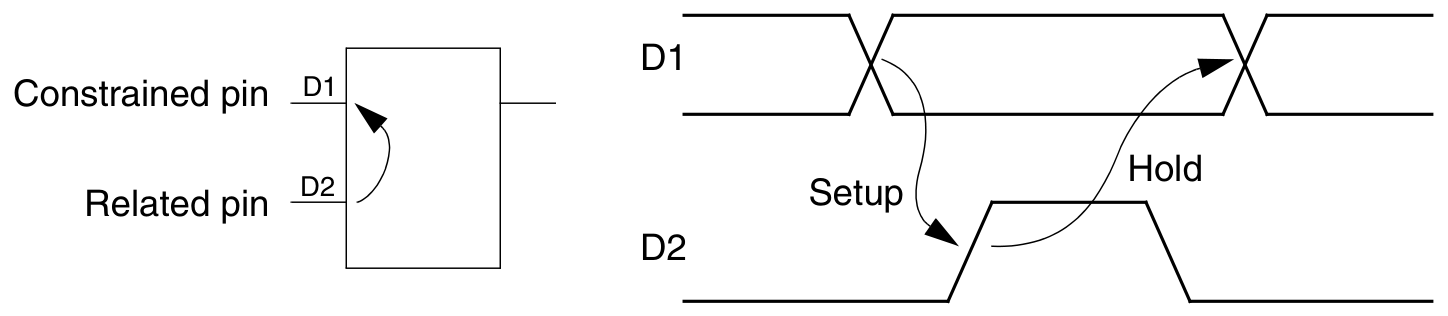
\includegraphics[width=0.9\textwidth]{fig-3-15.png}
  \caption{简单 data check 示例}
  \label{fig:3-15}
\end{figure}

在本例中，D1 上的信号必须在有效沿之前的一段 setup 时间内保持稳定，也必须在有效沿之后的一段 hold 时间内保持稳定。若库单元尚未定义这些 nonsequential 约束，可以用 \cmd{set\_data\_check} 在工具中定义。

data check 是非时序的，因此不会打断时序路径。在下图中，引脚 D1 与 D2 之间的 data check 不会中断虚线箭头所示的时序路径。若把 D2 上的信号定义为时钟，则该检查成为时序检查，路径在 D1 处终止。

\begin{figure}[htbp]
  \centering
  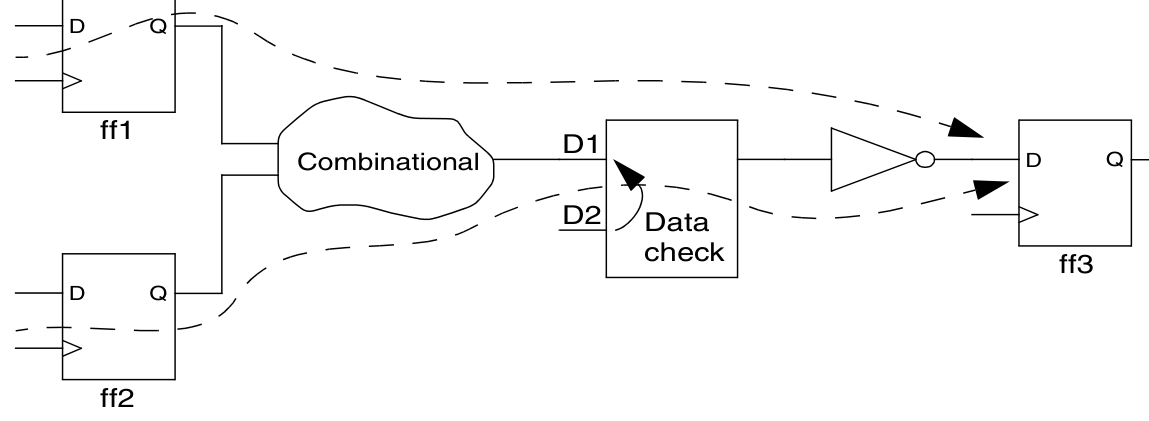
\includegraphics[width=0.9\textwidth]{fig-3-16.png}
  \caption{未被 data check 打断的时序路径}
  \label{fig:3-16}
\end{figure}

在 data check 中，到达被约束引脚或相关引脚的信号可以来自不同时钟域。工具分别检查这些信号路径，并把它们放入不同的时钟组，与普通时序检查相同。

\section{指定 data-to-data check}
\subsection*{Specifying Data-to-Data Checks}

要指定在两个数据引脚之间执行 data-to-data check，按下列方式使用 \cmd{set\_data\_check}：
\begin{itemize}
  \item 用 \opt{-from}、\opt{-rise\_from} 或 \opt{-fall\_from} 把引脚或端口指定为相关引脚。
  \item 用 \opt{-to}、\opt{-rise\_to} 或 \opt{-fall\_to} 把引脚或端口指定为被约束引脚。
  \item 用 \opt{-setup} 或 \opt{-hold} 指定 data check 值只用于 setup 或只用于 hold。否则该值同时用于 setup 与 hold。
  \item 用 \opt{-clock} 指定发射相关引脚上信号的那一个时钟的名称。
\end{itemize}

要去掉用 \cmd{set\_data\_check} 设置的 data check，使用 \cmd{remove\_data\_check}。

\subsection{data check 示例}
\subsubsection*{Examples of Data Checks}

在下图中，D1 上的信号必须在有效沿之前的一段 setup 时间内保持稳定，也必须在有效沿之后的一段 hold 时间内保持稳定。

\begin{figure}[htbp]
  \centering
  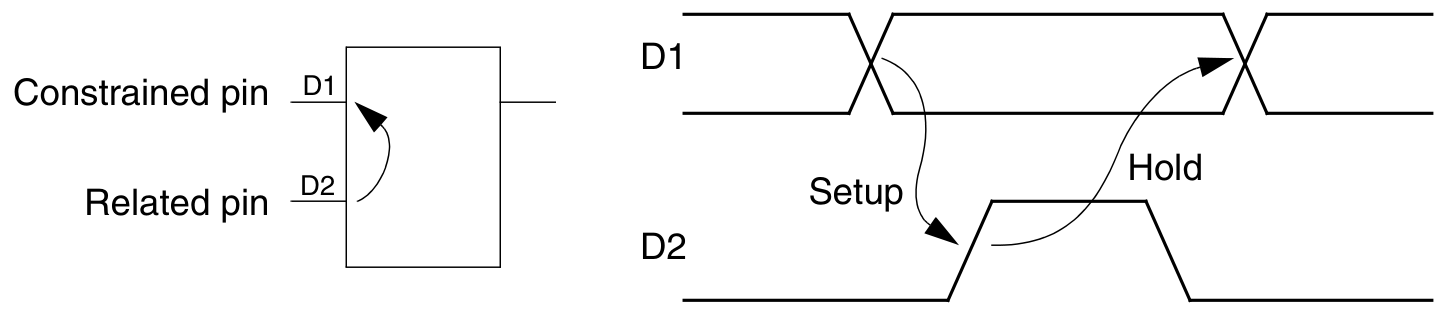
\includegraphics[width=0.9\textwidth]{fig-3-17.png}
  \caption{上升沿上的 data check}
  \label{fig:3-17}
\end{figure}

用下列命令定义这些 data check：
\begin{lstlisting}
icc2_shell> set_data_check -rise_from D2 -to D1 -setup 3.5
icc2_shell> set_data_check -rise_from D2 -to D1 -hold 6.0
\end{lstlisting}

在下图中，data check 同时作用于相关引脚的上升沿与下降沿。

\begin{figure}[htbp]
  \centering
  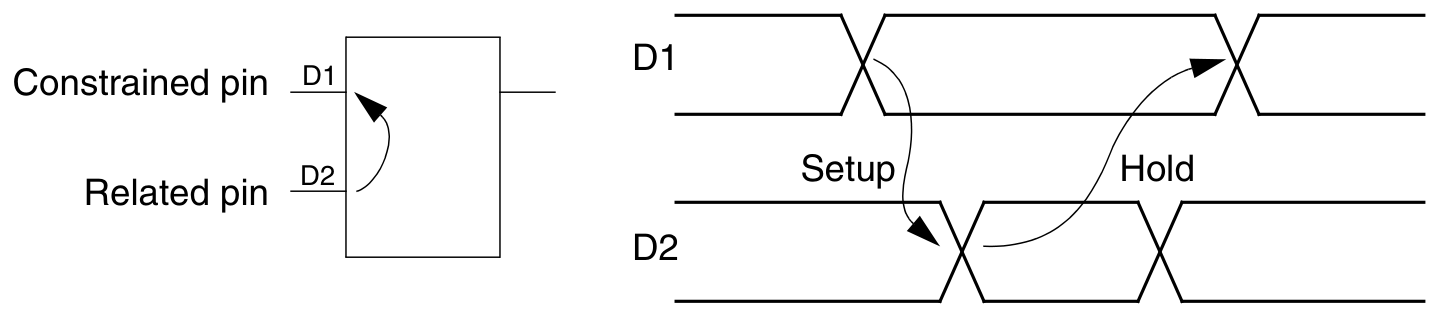
\includegraphics[width=0.9\textwidth]{fig-3-18.png}
  \caption{上升沿与下降沿上的 data check}
  \label{fig:3-18}
\end{figure}

用下列命令定义这些 data check：
\begin{lstlisting}
icc2_shell> set_data_check -from D2 -to D1 -setup 3.5
icc2_shell> set_data_check -from D2 -to D1 -hold 6.0
\end{lstlisting}

可以只指定从上升沿出发的 setup 检查和从下降沿出发的 hold 检查，从而定义 no-change data check，命令如下：
\begin{lstlisting}
icc2_shell> set_data_check -rise_from D2 -to D1 -setup 3.5
icc2_shell> set_data_check -fall_from D2 -to D1 -hold 3.0
\end{lstlisting}

工具把这解释为正脉冲上的 no-change 检查。得到的时序检查如下图所示。

\begin{figure}[htbp]
  \centering
  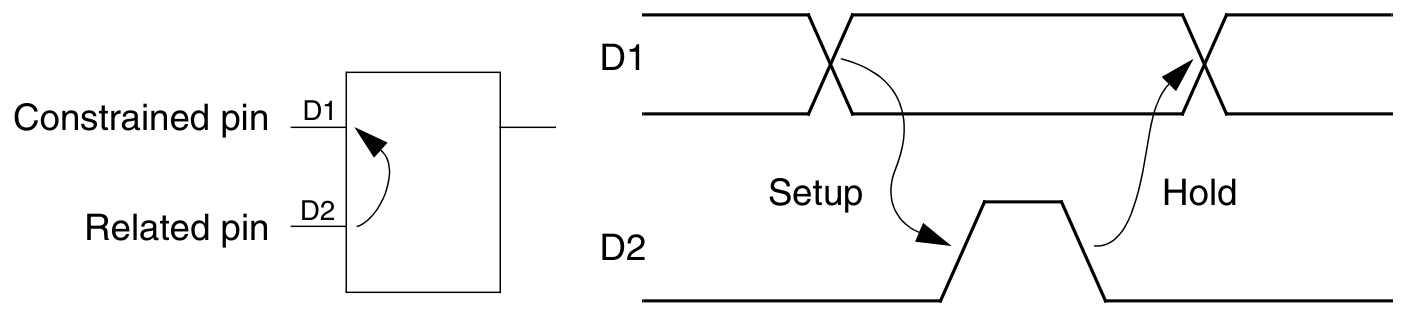
\includegraphics[width=0.9\textwidth]{fig-3-19.png}
  \caption{no-change data check}
  \label{fig:3-19}
\end{figure}

\section{使能基于库的 data check}
\subsection*{Enabling Library-Based Data Checks}

若相关引脚上的信号未被定义为时钟，要让工具对库单元中定义了 nonsequential 时序约束的任何单元执行 data check，把应用选项 \appopt{time.enable\_non\_sequential\_checks} 设为 \cmd{true}，如下例所示：
\begin{lstlisting}
icc2_shell> set_app_options -name time.enable_non_sequential_checks \
    -value true
\end{lstlisting}

该变量默认为 \cmd{false}。

\begin{noteBox}
这一行为与 PrimeTime 不同。PrimeTime 始终执行 nonsequential arc 检查。
\end{noteBox}

若相关引脚上的信号被定义为时钟，工具忽略库中定义的 nonsequential 时序约束。

在单元库中，单元的 nonsequential 约束通过指定相关引脚，并为被约束引脚赋予下列 \cmd{timing\_type} 属性来定义：
\begin{itemize}
  \item \cmd{non\_seq\_setup\_rising}
  \item \cmd{non\_seq\_setup\_falling}
  \item \cmd{non\_seq\_hold\_rising}
  \item \cmd{non\_seq\_hold\_falling}
\end{itemize}

\begin{seeAlsoBox}
关于在库中定义 nonsequential 约束的更多信息，参见 Library Compiler 文档。
\end{seeAlsoBox}

使用库单元中定义的 nonsequential 约束，比使用 \cmd{set\_data\_check} 得到的分析更准确，因为 setup 与 hold 时间可以随被约束引脚和相关引脚的 slew 变化。\cmd{set\_data\_check} 对 slew 不敏感。

\cmd{remove\_data\_check} 不会去掉库单元中定义的 data check。

\section{时钟门控检查简介}
\subsection*{Introduction to Clock-Gating Checks}

当时钟网络中含有反相器或缓冲器以外的逻辑时，就出现门控时钟信号。工具不会自动检查时钟门控单元的门控信号上的 setup 与 hold 违例。因此，这些信号有可能在时钟脉冲穿过门控单元时发生跳变，从而既产生被削窄的时钟脉冲，也产生虚假的时钟脉冲。

下图给出：在没有时钟门控检查时，时钟门控输入上的非法变化可能造成的畸变时钟波形。

\begin{figure}[htbp]
  \centering
  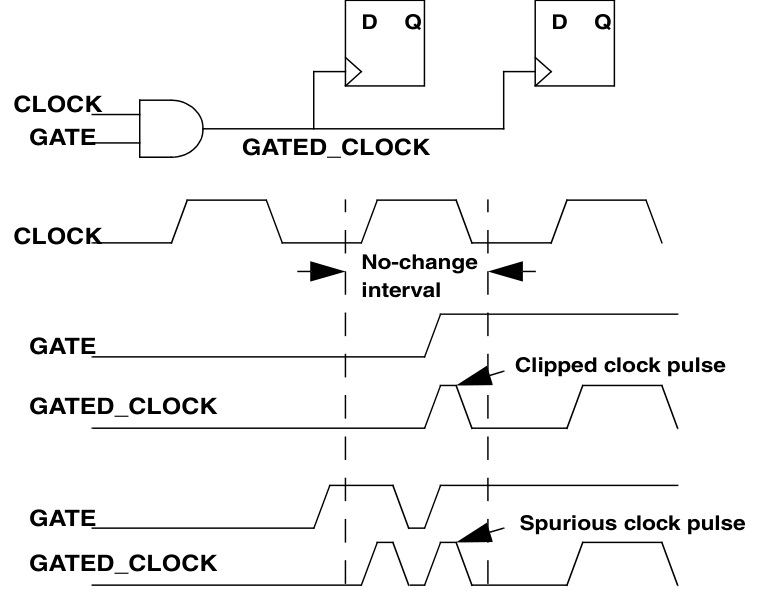
\includegraphics[width=0.9\textwidth]{fig-3-20.png}
  \caption{畸变的时钟波形}
  \label{fig:3-20}
\end{figure}

要控制门控信号的跳变，可以用 \cmd{set\_clock\_gating\_check} 相对于时钟指定 setup 裕量与 hold 裕量。

下图给出在作为门控元件的 AND 或 NAND 门上执行的时钟门控检查。

\begin{figure}[htbp]
  \centering
  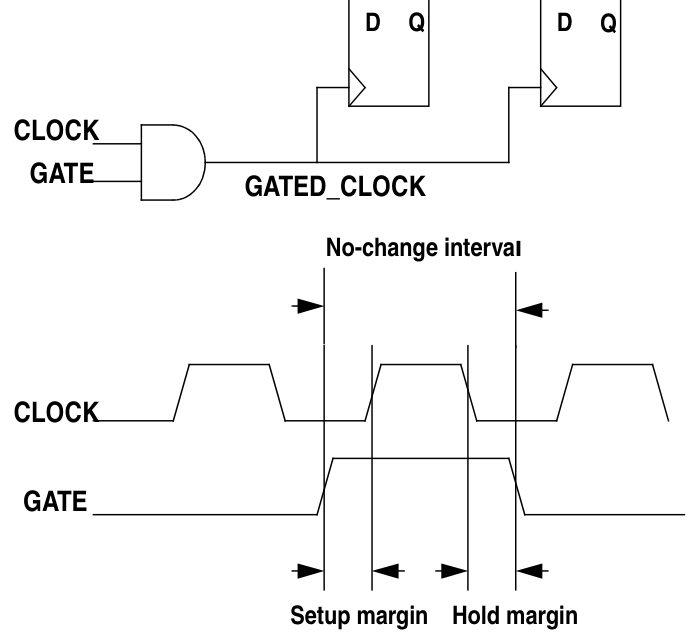
\includegraphics[width=0.9\textwidth]{fig-3-21.png}
  \caption{AND 与 NAND 门的时钟门控检查}
  \label{fig:3-21}
\end{figure}

下图给出在作为门控元件的 OR 或 NOR 门上执行的时钟门控检查。

\begin{figure}[htbp]
  \centering
  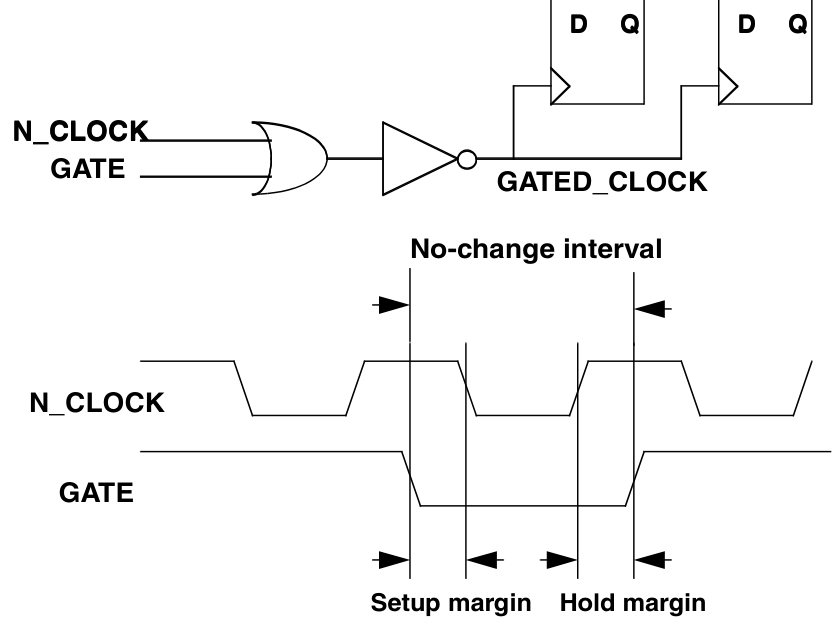
\includegraphics[width=0.9\textwidth]{fig-3-22.png}
  \caption{OR 与 NOR 门的时钟门控检查}
  \label{fig:3-22}
\end{figure}

\section{指定时钟门控检查}
\subsection*{Specifying Clock-Gating Checks}

要指定时钟门控检查，使用 \cmd{set\_clock\_gating\_check}。

使用该命令时，工具默认：
\begin{itemize}
  \item 对当前 block 的全部时钟门控元件执行时钟门控检查。\\
        要把检查限制到指定单元、指定时钟，或某个端口或引脚的传递扇出（transitive fanout），指定所需对象。
  \item 使用的 setup 与 hold 值为零。要设置具体的 setup 或 hold 值，使用 \opt{-setup} 或 \opt{-hold}。
  \item 同时约束门控信号的上升沿与下降沿。\\
        若只控制上升沿或下降沿，使用 \opt{-rise} 或 \opt{-fall}。
  \item 根据门控逻辑，决定用时钟的高电平还是低电平来约束门控信号。\\
        若门控单元是：
        \begin{itemize}
          \item AND 或 NAND 门，工具在时钟的高电平上执行检查。
          \item OR 或 NOR 门，工具在时钟的低电平上执行检查。
          \item 其他门，除非指定使用时钟的哪一个电平，否则工具不执行检查。
        \end{itemize}
        要指定在时钟的哪一个电平上执行检查，使用 \opt{-high} 或 \opt{-low}。
\end{itemize}

工具像处理其他时序约束一样处理时钟门控检查，并尝试调整驱动门控输入的逻辑延迟，以避免 setup 与 hold 违例。优化期间，对带有时钟门控检查的单元，工具只能调整尺寸。

时钟门控检查只能在一个时钟信号与一个非时钟信号之间进行，不能在两个时钟信号之间进行，也不能在两个非时钟信号之间进行。

要去掉时钟门控检查，使用 \cmd{remove\_clock\_gating\_check}。

可以用 \cmd{set\_disable\_clock\_gating\_check} 列出希望工具忽略的单元和引脚，从而在指定单元和引脚上禁用时钟门控检查。要取消该命令的作用，使用 \cmd{remove\_disable\_clock\_gating\_check}。

下例说明如何在 CLK1 时钟网络中的全部门上指定 setup 要求 0.2 与 hold 要求 0.4。
\begin{lstlisting}
icc2_shell> set_clock_gating_check -setup 0.2 -hold 0.4 CLK1
\end{lstlisting}

% 第 4 章 Specifying Operating Conditions
\bichapter{指定工作条件}{Specifying Operating Conditions}
\label{chap:ocv}

工作条件包括芯片工作时的工艺、电压与温度参数。可以为 block 指定工作条件，工具在这些条件下分析并优化 block。

默认情况下，工具用片上变异（on-chip variation，OCV）模式做时序分析，以建模芯片上工作条件的变化。工具还支持高级片上变异（advanced on-chip variation，AOCV），作为提高时序分析精度的可选方法。

本章包括以下主题：
\begin{itemize}
  \item 指定工作条件
  \item 用工艺标签做 PVT 匹配
  \item 报告 PVT 信息
  \item 片上变异延迟分析
  \item 指定时序 derating 因子
  \item AOCV 简介
  \item 为 AOCV 分析做准备
  \item 施加 AOCV 数据
  \item 基于文件的 AOCV 数据
  \item 验证 AOCV 数据
  \item 参数化片上变异分析简介
  \item POCV 数据格式
  \item 执行参数化片上变异分析
  \item 时钟再汇聚悲观量消除简介
  \item 启用时钟再汇聚悲观量消除
  \item 报告时钟再汇聚悲观量消除的计算
\end{itemize}

\section{指定工作条件}
\subsection*{Specifying the Operating Conditions}

block 的工作条件包括芯片工作时所处的工艺、电压与温度。IC Compiler II 在所指定的条件下分析并优化 block。early 分析与 late 分析可以使用同一组或不同的工作条件。

指定工作条件有两种方法。

\begin{itemize}
  \item 分别指定下列参数：
  \begin{itemize}
    \item 用 \cmd{set\_process\_number} 指定工艺因子。默认同时作用于 early 与 late 分析。若只给其中一种分析指定数值，使用 \opt{-early} 或 \opt{-late}。
    \item 用 \cmd{set\_voltage} 指定电压。默认同时作用于 early 与 late。若 early 分析要用不同数值，使用 \opt{-min}。
    \item 用 \cmd{set\_temperature} 指定温度。默认同时作用于 early 与 late。若 early 分析要用不同数值，使用 \opt{-min}。
  \end{itemize}
        这些命令默认作用于当前 corner 上 block 内的全部对象。可用 \opt{-corners} 指定受影响的 corner，用 \opt{-object\_list} 指定受影响的对象。
  \item 用 \cmd{set\_operating\_conditions} 指定工作条件。所指定的工作条件：
  \begin{itemize}
    \item 同时作用于 early 与 late 分析。若只用于其中一种，使用 \opt{-min} 或 \opt{-max}。
    \item 只作用于当前 corner。对多 corner 多 mode 设计，必须为 block 中每个 corner 指定工作条件。
  \end{itemize}
\end{itemize}

参考库可以包含多组工作条件。用 \cmd{report\_lib} 列出某个库中可用的工作条件并查看其特征。

一般只使用一种方法为 block 指定工作条件。若必须两种都用，例如为多电压设计设置工作电压以覆盖 SDC 文件中的工作条件，先用 \cmd{set\_operating\_conditions}，再用单条命令覆盖具体数值。

\begin{seeAlsoBox}
\textit{IC Compiler II Library Preparation User Guide}
\end{seeAlsoBox}

\section{用工艺标签做 PVT 匹配}
\subsection*{Using Process Labels for PVT Matching}

参考库中的单元可以针对一种或多种工作条件做特性化。对 block 中的门级单元做时序分析时，若为 block 指定的工作条件与参考库中该单元的工作条件完全匹配，工具使用该数据；否则使用最接近的匹配。

\begin{noteBox}
若参考库含有 scaling group，scaling group 内的插值被视为精确匹配。
\end{noteBox}

可以用工艺标签（process label）引导工具从参考库中选择合适的时序模型。工艺标签在库准备期间加到参考库的特性化点上，例如：
\begin{lstlisting}
icc2_lm_shell> read_db -process_label fast fast_lib_0p95v125c.db
\end{lstlisting}

要引导 IC Compiler II 对某个 corner 使用指定的特性化点，用 \cmd{set\_process\_label} 为该 corner 指定工艺标签：
\begin{lstlisting}
icc2_shell> create_corner c_fast
icc2_shell> set_process_label -corners c_fast fast
\end{lstlisting}

\section{报告 PVT 信息}
\subsection*{Reporting PVT Information}

用 \cmd{report\_pvt} 报告 PVT 信息，包括为 corner 指定的工作条件与 block 中所用单元时序视图之间的不匹配。报告包含所指定的 PVT 设置，以及找不到精确匹配时所实际使用的设置。

除 \cmd{report\_pvt} 外，还可以通过查询表~\ref{tab:pvt-attr} 中的时序属性，取得当前 block 所用的 PVT 值。

\begin{table}[htbp]
\centering
\caption{工作条件属性}
\label{tab:pvt-attr}
\small
\begin{tabularx}{\textwidth}{@{}l *{3}{>{\raggedright\arraybackslash}X}@{}}
\toprule
设置 & 指定值 & 解析值 & 不匹配计数 \\
\midrule
工艺标签 &
\cmd{process\_label\_early}\newline
\cmd{process\_label\_late} &
\cmd{effective\_process\_label\_early}\newline
\cmd{effective\_process\_label\_late} &
\cmd{process\_label\_mismatches} \\
工艺数值 &
\cmd{process\_number\_early}\newline
\cmd{process\_number\_late} &
\cmd{effective\_process\_number\_early}\newline
\cmd{effective\_process\_number\_late} &
\cmd{process\_number\_mismatches} \\
电压 &
\cmd{voltage\_early}\newline
\cmd{voltage\_late} &
\cmd{effective\_voltage\_early}\newline
\cmd{effective\_voltage\_late} &
\cmd{voltage\_mismatches} \\
温度 &
\cmd{temperature\_early}\newline
\cmd{temperature\_late} &
\cmd{effective\_temperature\_early}\newline
\cmd{effective\_temperature\_late} &
\cmd{temperature\_mismatches} \\
\bottomrule
\end{tabularx}
\end{table}

\section{片上变异延迟分析}
\subsection*{On-Chip Variation Delay Analysis}

时序分析期间，工具使用 OCV 模式。该模式同时把最小延迟与最大延迟加到不同路径上，从而做偏保守的时序分析。

对 setup 检查，工具对 launch 时钟路径与数据路径使用最大延迟，对 capture 时钟路径使用最小延迟，如图~\ref{fig:ocv-setup}。

\begin{figure}[htbp]
  \centering
  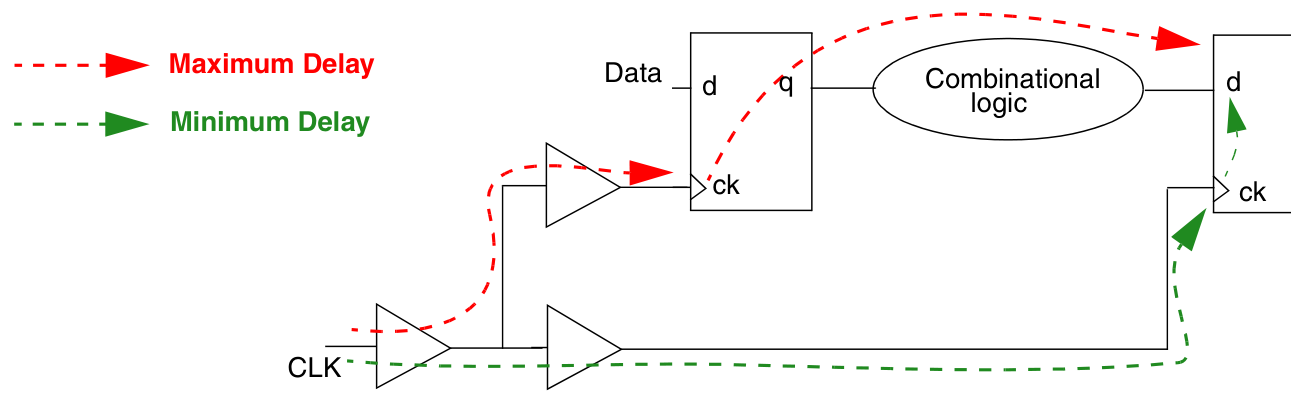
\includegraphics[width=0.88\textwidth]{fig-4-1.png}
  \caption{setup 分析中的片上变异}
  \label{fig:ocv-setup}
\end{figure}

对 hold 检查，工具对 launch 时钟路径与数据路径使用最小延迟，对 capture 时钟路径使用最大延迟，如图~\ref{fig:ocv-hold}。

\begin{figure}[htbp]
  \centering
  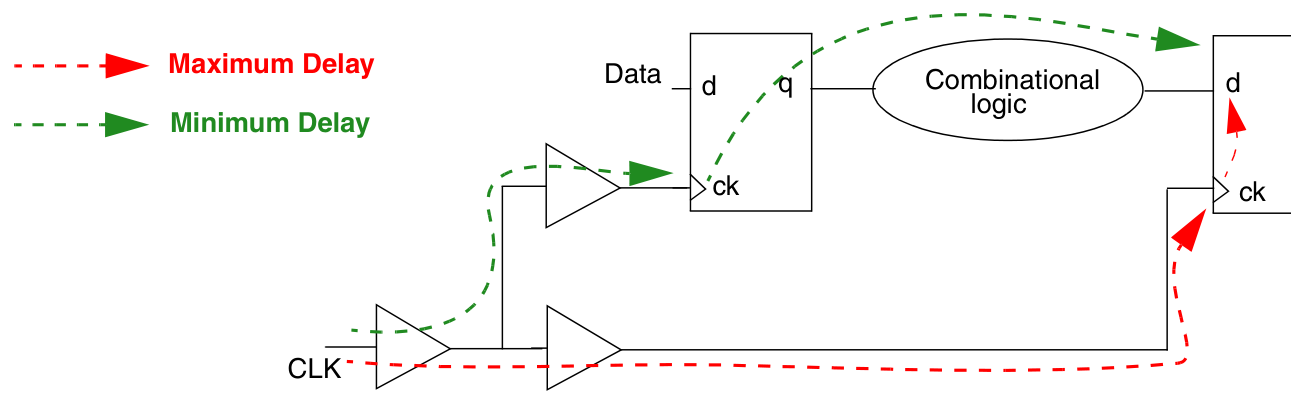
\includegraphics[width=0.88\textwidth]{fig-4-2.png}
  \caption{hold 分析中的片上变异}
  \label{fig:ocv-hold}
\end{figure}

表~\ref{tab:setup-hold-params} 给出 setup 检查与 hold 分析所用的时钟到达时间、延迟、工作条件与 derating。

\begin{table}[htbp]
\centering
\caption{setup 与 hold 分析所用的时序参数}
\label{tab:setup-hold-params}
\begin{tabularx}{\textwidth}{@{}l X X X@{}}
\toprule
分析类型 & Launch 时钟路径 & 数据路径 & Capture 时钟路径 \\
\midrule
Setup &
Late 时钟，时钟路径最大延迟，late derating，最坏情况工作条件 &
最大延迟，late derating，最大工作条件 &
Early 时钟，时钟路径最小延迟，early derating，最小工作条件 \\
Hold &
Early 时钟，时钟路径最小延迟，early derating，最好情况工作条件 &
最小延迟，early derating，最小工作条件 &
Late 时钟，时钟路径最大延迟，late derating，最大工作条件 \\
\bottomrule
\end{tabularx}
\end{table}

时序分析期间，工具同时考虑下列设计参数所指定的最小值与最大值：输入与输出外部延迟、端口线负载模型、端口扇出数、网线电容、网线电阻、网线线负载模型、时钟 latency、时钟转换时间，以及输入端口的驱动单元。

\section{指定时序 derating 因子}
\subsection*{Specifying the Timing Derating Factors}

时序 derating 因子通过调整 block 中各时序弧的计算延迟，建模工作条件变化的影响。默认 derating 因子为 1.0，工具不调整计算得到的延迟。

用 \cmd{set\_timing\_derate} 设置 derating 因子，并指定：
\begin{itemize}
  \item derating 因子本身。
  \item 用 \opt{-early} 或 \opt{-late} 说明该因子用于 early 还是 late 延迟。
\end{itemize}

还可以把 derating 因子施加到：
\begin{itemize}
  \item 指定的叶级实例、层次实例或库单元。默认作用于当前 block。
  \item 只用 \opt{-rise} 或 \opt{-fall} 作用于上升或下降延迟。默认同时作用于两者。
  \item 只用 \opt{-clock} 或 \opt{-data} 作用于时钟路径或数据路径。默认同时作用于两者。
  \item 用 \opt{-net\_delay}、\opt{-cell\_delay} 或 \opt{-cell\_check} 作用于网线延迟、单元延迟或单元时序检查。默认三者都作用。用 \cmd{set\_timing\_derate -net\_delay} 为网线延迟指定 derating 时，同时作用于网线延迟的动态分量与静态分量。可用 \opt{-dynamic} 与 \opt{-static} 为两个分量指定不同因子。
  \item 用 \opt{-corners} 作用于指定 corner。默认作用于当前 corner。
\end{itemize}

要用增量修改已有 timing derate，使用 \opt{-increment}。该增量加到已有 derating 因子上。

下例把当前 corner 的全部最小延迟减小 10\%，全部最大延迟增大 20\%：
\begin{lstlisting}
icc2_shell> set_timing_derate -early 0.9 -late 1.2
\end{lstlisting}

用 \cmd{report\_timing\_derate} 报告 derating 因子。默认报告全部 corner；用 \opt{-corners} 报告指定 corner。

用 \cmd{reset\_timing\_derate} 把 derating 因子复位为 1.0。默认复位当前 corner 上当前 block 及其全部单元实例的因子。用 \opt{-corners} 复位指定 corner，或指定对象以复位这些对象上的因子。

\section{AOCV 简介}
\subsection*{Introduction to AOCV}

高级片上变异（AOCV）是一种可选方法：按路径深度或物理距离跨度，对不同路径使用不同的 derating 因子，从而提高精度。逻辑级数更多或物理距离更长的路径，总变异往往更小，因为门与门之间的随机变异趋于相互抵消。因此 AOCV 对短路径使用较高的 derating，对长路径使用较低的 derating。

这种方法比传统 OCV 更不悲观。传统 OCV 依赖不考虑路径具体度量的常数 derating。精度提高会同时影响时序报告与设计优化。

IC Compiler II 的 AOCV 流程包括以下高层步骤：
\begin{enumerate}
  \item 按「为 AOCV 分析做准备」设置 AOCV 分析。
  \item 按「施加 AOCV 数据」施加 AOCV 数据。
  \item 按「验证 AOCV 数据」验证 AOCV 数据。
  \item 使用 AOCV 数据做时序分析与优化。
\end{enumerate}

\section{为 AOCV 分析做准备}
\subsection*{Setting Up for AOCV Analysis}

把应用选项 \appopt{time.aocvm\_enable\_analysis} 设为 \cmd{true} 以启用 AOCV 分析。

还可以用下列应用选项改变默认行为：
\begin{itemize}
  \item 把 \appopt{time.aocvm\_enable\_clock\_network\_only} 设为 \cmd{true}，使 AOCV 只分析时钟网络。默认同时分析时钟网络与数据网络。
  \item 用 \appopt{time.aocvm\_analysis\_mode} 改变 AOCV 分析中路径深度的计算方式，有三种设置：
  \begin{itemize}
    \item \cmd{separate\_launch\_capture\_depth}：默认。同时使用时钟与数据网络对象，并为 capture 路径与 launch 路径分别计算深度。
    \item \cmd{combined\_launch\_capture\_depth}：同时使用时钟与数据网络对象，把 capture 与 launch 合在一起计算整条路径的深度。
    \item \cmd{separate\_data\_and\_clock\_metrics}：为时钟路径与数据路径分别计算深度。
  \end{itemize}
  \item 把 \appopt{time.ocvm\_enable\_distance\_analysis} 设为 \cmd{true}，在门计数之外再考虑物理距离。默认不考虑路径的物理距离。
  \item 把 \appopt{time.aocvm\_enable\_single\_path\_metrics} 设为 \cmd{true}，只用单元距离与深度度量来导出单元和网线的 AOCV derating。
  \item 把 \appopt{time.ocvm\_precedence\_compatibility} 设为 \cmd{true}，当存在 AOCV derating 时忽略由 \cmd{set\_timing\_derate} 指定的 OCV derating。默认同时考虑 OCV 与 AOCV，优先级从高到低为：
  \begin{enumerate}
    \item 叶单元上的 OCV derate
    \item 库单元上的 AOCV derate
    \item 库单元上的 OCV derate
    \item 层次单元上的 AOCV derate
    \item 层次单元上的 OCV derate
    \item 设计上的 AOCV derate
    \item 设计上的 OCV derate
  \end{enumerate}
\end{itemize}

\section{施加 AOCV 数据}
\subsection*{Applying AOCV Data}

AOCV 时序分析期间，工具根据路径中相继的门数（路径深度），以及可选的路径物理距离跨度，从 AOCV 数据导出 derating 值。

提供 AOCV 数据有两种方法：
\begin{itemize}
  \item 使用逻辑库（\cmd{.db}）中基于库的 AOCV 数据。
  \item 使用基于文件的 AOCV 数据，用 \cmd{read\_ocvm} 读入。
\end{itemize}

用 \opt{-corners} 为指定 corner 施加 AOCV 数据。基于库与基于文件的 AOCV 数据都可以由 Synopsys SiliconSmart 特性化工具生成。细节见 SolvNet 上的 \textit{SiliconSmart ACE User Guide}。

可以同时使用基于库与基于文件的 AOCV derating。冲突时优先级从高到低为：
\begin{enumerate}
  \item 库单元上基于文件的 AOCV derate
  \item 层次单元上基于文件的 AOCV derate
  \item 设计上基于文件的 AOCV derate
  \item 库单元或库上基于库的 AOCV derate
\end{enumerate}

还可以指定：
\begin{itemize}
  \item 用 \cmd{set\_timing\_derate -aocvm\_guardband} 为 AOCV derating 因子设置保护带。下例为 early 与 late 延迟指定 5\% 的保护带：
\begin{lstlisting}
icc2_shell> set_timing_derate -aocvm_guardband -early 0.95
icc2_shell> set_timing_derate -aocvm_guardband -late 1.05
\end{lstlisting}
  \item 用 \cmd{set\_aocvm\_coefficient} 在库单元或单元实例级设置深度调整系数。计算时序路径总深度（逻辑级数）时，工具默认把每个单元的深度计为 1。该命令可以增大或减小某个库单元的深度。下例把库单元 \cmd{MGX16} 的深度增至 1.5：
\begin{lstlisting}
icc2_shell> set_aocvm_coefficient 1.5 [get_lib_cells lib_fast/MGX16]
\end{lstlisting}
\end{itemize}

用 \cmd{remove\_ocvm} 从设计对象上去掉部分或全部 AOCV derating 值。

\section{基于文件的 AOCV 数据}
\subsection*{File-Based AOCV Data}

AOCV 数据文件把单元、库单元或网线的 derating 值指定为路径深度的函数，可选地也是路径所跨越物理距离的函数。IC Compiler II 接受 PrimeTime 中 \cmd{write\_binary\_aocvm} 产生的二进制与压缩数据文件。

表~\ref{tab:aocv-fmt} 给出 AOCV 文件格式的语法。

\begin{table}[htbp]
\centering
\caption{AOCV 文件格式语法}
\label{tab:aocv-fmt}
\begin{tabularx}{\textwidth}{@{}l X@{}}
\toprule
字段 & 说明 \\
\midrule
\cmd{version} & AOCV 版本号 \\
\cmd{object\_type} & \cmd{design | cell | lib\_cell} \\
\cmd{rf\_type} & \cmd{rise | fall | rise fall} \\
\cmd{delay\_type} & \cmd{cell | net | cell net} \\
\cmd{derate\_type} & \cmd{early | late} \\
\cmd{path\_type} & \cmd{clock | data | clock data} \\
\cmd{object\_spec} & 字符串 \\
\cmd{depth} & 一组 $M$ 个浮点数，$M$ 可以为 0 \\
\cmd{distance} & 一组 $N$ 个浮点数，$N$ 可以为 0。只有 \appopt{time.ocvm\_enable\_distance\_analysis} 为 \cmd{true} 时才使用距离值 \\
\cmd{table} & 一组 $N \times M$ 个浮点数。特殊情况：$N=0$ 时表的大小为 $M$；$M=0$ 时表的大小为 $N$；两者都为 0 时表的大小为 1。未定义的点用线性插值。工具不外推到表中最低值或最高值之外 \\
\bottomrule
\end{tabularx}
\end{table}

\cmd{object\_spec} 指定对象名。还可以使用按对象属性求值的表达式，类似于在创建 collection 的命令中使用 Tcl 的 \cmd{regexp}。\cmd{patterns} 字段可以使用相关 collection 命令的任意选项。例如 \cmd{object\_type} 为 \cmd{lib\_cell} 时，可以使用 \cmd{get\_lib\_cells} 的任意参数。

在文件任意位置加注释时，使用双斜杠（\cmd{//}）。

下例为整个设计中的时钟网线设置 early AOCV 表：
\begin{lstlisting}
version             1.0
object_type:        design
rf_type:            rise fall
delay_type:         cell net
derate_type:        early
path_type:          clock
object_spec:        top
depth:              0 1 2 3
distance:           100 200
table:              0.87 0.93 0.95 0.96 \
                    0.83 0.85 0.87 0.90
\end{lstlisting}

下例为工作条件电压为 1.2~V 的全部层次单元、时钟路径设置 late AOCV 表：
\begin{lstlisting}
version             1.0
object_type:        cell
rf_type:            rise
delay_type:         cell
derate_type:        late
path_type:          clock
object_spec:        * -filter (voltage_max==1.2 && is_hierarchical==true)
depth:              1  2  3
distance:           100  1000
table:              1.21  1.11  1.09 \
                    1.23  1.16  1.14
\end{lstlisting}

\section{验证 AOCV 数据}
\subsection*{Verifying AOCV Data}

用 \cmd{report\_ocvm} 查看 AOCV derate 表。可以查看标注了 early、late、rise、fall、cell 或 net derate 表的设计对象，也可以用该命令判断哪些单元和网线已标注或尚未标注 AOCV 信息。

例如，取得单元 \cmd{U57} 从引脚 A 到引脚 Z 的时序弧上的 AOCV derate 数据：
\begin{lstlisting}
icc2_shell> report_ocvm -type ocvm \
    [get_timing_arcs -from U57/I -to U57/Z]
\end{lstlisting}

\section{参数化片上变异分析简介}
\subsection*{Introduction to Parametric On-Chip Variation Analysis}

参数化片上变异（parametric on-chip variation，POCV）分析是一种可选的时序分析模式，用统计方法建模片上变异。在该模式下，工具把到达时间、要求时间与 slack 计算为统计分布，而不是固定的最小与最大值。时序结果更不悲观，为时序优化提供更好的依据。

POCV 时序分析不为每条时序弧指定绝对的最小与最大延迟，而是把延迟表示为高斯（正态）分布 $P$ 的函数：
\[
\mathrm{delay} = \mathrm{nominal\_delay} + \sigma \cdot P
= \mathrm{nominal\_delay} + (C \cdot \mathrm{nominal\_delay}) \cdot P
\]

工具从 \cmd{.db} 库取得延迟变异 $\sigma$（若库中有），或由 POCV 数据文件中提供的系数 $C$ 计算，其中 $\sigma = C \cdot \mathrm{nominal\_delay}$。

图~\ref{fig:pocv} 把传统 min-max 延迟与 POCV 统计延迟作图形比较。

\begin{figure}[htbp]
  \centering
  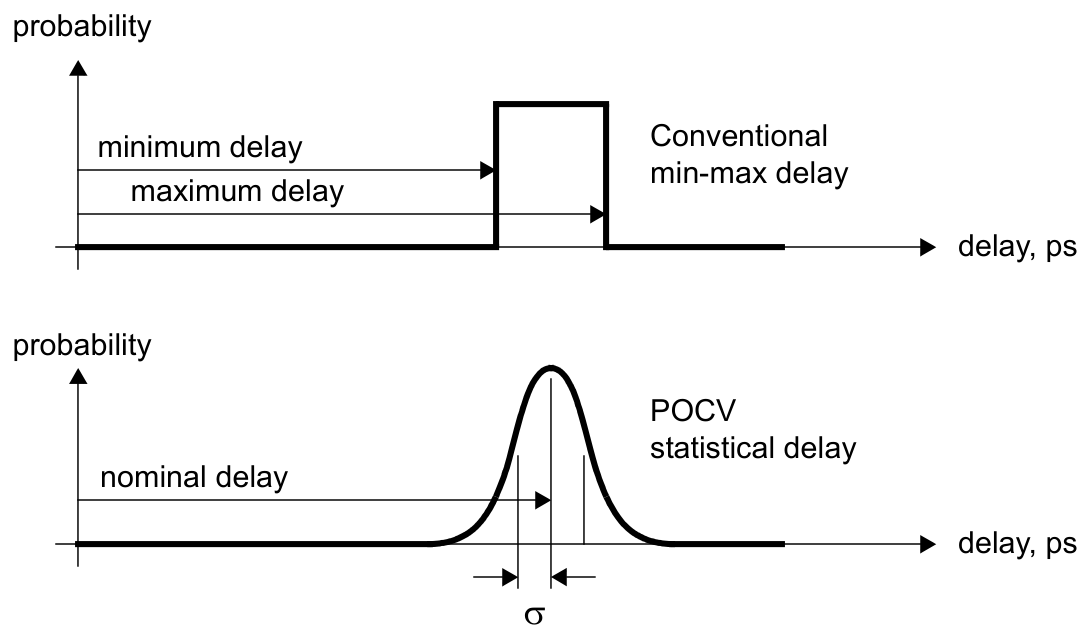
\includegraphics[width=0.78\textwidth]{fig-4-3.png}
  \caption{min-max 延迟与 POCV 统计延迟的比较}
  \label{fig:pocv}
\end{figure}

两种延迟变异的差别：
\begin{itemize}
  \item min-max 延迟为时序弧指定绝对最小与最大延迟。实际延迟在这两个极端之间任意位置出现的概率相等，超出这两个极端的概率为零。
  \item POCV 统计模型指定标称延迟与变异 $\sigma$。延迟在标称值处出现的概率最高，离标称值越远概率越小。实际延迟落在标称延迟 $3\sigma$ 范围内的概率为 99.7\%。
\end{itemize}

工具确定每条时序弧的延迟分布之后，沿时序路径做统计传播，把每个到达时间、要求时间与 slack 计算为总标称值加上累积变异。

计算路径累积延迟时，工具把每一级的延迟分布做统计合并。这比简单地把每一级的最坏情况值相加更准确。得到的延迟与 slack 比简单的 min-max 相加更现实、更不悲观。

默认情况下，\cmd{report\_timing} 报告的最终 slack 是比标称 slack 低三个标准差（$3\sigma$）的 slack：
\[
\mathrm{reported\_slack} = \mathrm{nominal\_slack} - 3\sigma
\]

可以把 sigma 乘数从 3.0 改大或改小，以收紧或放宽时序约束。

\section{POCV 数据格式}
\subsection*{POCV Data Formats}

执行 POCV 时序分析时，IC Compiler II 需要每条时序弧的变异 $\sigma$。提供该信息有两种方式。

\begin{itemize}
  \item \textbf{基于库的 POCV 数据}\\
        工具支持 Liberty Variation Format（LVF）中、基于 \cmd{.db} 库的 POCV 变异数据，覆盖延迟、转换时间与约束弧。
  \begin{itemize}
    \item 对延迟弧，每个 LVF 表项给出输入 slew 与输出负载某一组合下的延迟变异 $\sigma$。
    \item 对转换时间弧，每个 LVF 表项给出输入 slew 与输出负载某一组合下的转换时间变异 $\sigma$。
    \item 对约束弧，每个 LVF 表项给出被约束引脚与相关引脚转换时间某一组合下的约束变异 $\sigma$。
  \end{itemize}
\end{itemize}

\begin{noteBox}
若库中含有 LVF 表，请确认 IC Compiler II 设计库是用 K-2015.06-SP1 或更新版本的 IC Compiler II Library Manager 创建的。LVF 信息包含在设计库中，并在进入 IC Compiler II 会话时自动读入。
\end{noteBox}

\begin{itemize}
  \item \textbf{基于文件的 POCV 数据}\\
        用 \cmd{read\_ocvm} 为指定 corner 读入纯文本系数数据文件。系数文件含延迟变异数据，但不支持转换时间或约束变异数据。文件为文本中指定的每个库单元、层次单元或设计施加单一系数 $C$。延迟变异按 $\sigma = C \cdot \mathrm{nominal\_delay}$ 计算。一个单元的全部时序弧共用同一个系数 $C$，与输入 slew 和输出负载无关。
\end{itemize}

基于库与基于文件的 POCV 数据都可以由 SiliconSmart 生成。细节见 SolvNet 上的 \textit{SiliconSmart ACE User Guide}。

\subsection{基于文件的 POCV 数据}
\subsubsection*{File-Based POCV Data}

POCV 数据文件为设计、设计中的层次单元或设计所用的库单元指定延迟变异系数 $C$。工具接受 PrimeTime 中 \cmd{write\_binary\_aocvm} 产生的二进制与压缩数据文件。转换时间与约束变异必须使用基于 LVF 库的数据。POCV 分析始终同时作用于数据路径与时钟路径。

表~\ref{tab:pocv-fmt} 给出 POCV 数据文件的语法。

\begin{table}[htbp]
\centering
\caption{POCV 数据文件语法}
\label{tab:pocv-fmt}
\begin{tabularx}{\textwidth}{@{}l X@{}}
\toprule
字段 & 说明 \\
\midrule
\cmd{version} & 4.0（片上变异数据文件版本号，必须为 4.0 或更高） \\
\cmd{ocvm\_type} & \cmd{pocv}（参数化片上变异） \\
\cmd{object\_type} & \cmd{design | cell | lib\_cell} \\
\cmd{rf\_type} & \cmd{rise | fall | rise fall} \\
\cmd{delay\_type} & \cmd{cell | net | cell net} \\
\cmd{derate\_type} & \cmd{early | late} \\
\cmd{path\_type} & \cmd{clock | data | clock data} \\
\cmd{object\_spec} & 标注了 POCV 系数的对象名 \\
\cmd{coefficient} & 变异系数 \\
\bottomrule
\end{tabularx}
\end{table}

下例为库单元 \cmd{lib28/invx2} 的下降转换设置 POCV 系数：
\begin{lstlisting}
version:      4.0
ocvm_type:    pocvm
object_type:  lib_cell
rf_type rise: fall
delay_type :  cell
derate_type:  early
object_spec:  lib28/invx2
coefficient:  0.05
\end{lstlisting}

\cmd{object\_spec} 指定对象名，用法与 AOCV 文件相同：可按对象属性求值，并使用相关 collection 命令的选项。注释使用 \cmd{//}。

下例为整个设计的 early 延迟设置 POCV 系数：
\begin{lstlisting}
version:      4.0
ovcm_type:    pocv
object_type:  design
rf_type:      rise fall
delay_type:   cell net
derate_type:  early
object_spec:         // Leave object_spec blank if object_type is design
coefficient:  0.05
\end{lstlisting}

下例为工作条件电压为 1.2~V 的全部层次单元的 late 延迟设置 POCV 系数：
\begin{lstlisting}
version       4.0
ovcm_type:    pocv
object_type:  cell
rf_type:      rise
delay_type:   cell
derate_type:  late
object_spec:  * -filter (voltage_max==1.2 && is_hierarchical==true)
coefficient:  0.07
\end{lstlisting}

\subsection{文件 POCV 数据与库 POCV 数据的优先级}
\subsubsection*{Precedence of File- and Library-POCV Data}

可以同时使用基于文件与基于库的 POCV 数据。默认按下列优先级解决冲突，从高到低：
\begin{enumerate}
  \item 库单元上基于文件的 POCV 系数
  \item 层次单元上基于文件的 POCV 系数
  \item 设计上基于文件的 POCV 系数
  \item 库单元或库上基于库的 POCV LVF 数据
\end{enumerate}

用应用选项 \appopt{time.pocvm\_precedence} 改变默认优先级。默认值为 \cmd{file}。

\begin{itemize}
  \item 设为 \cmd{library} 时，优先级为：库单元或库上的 LVF 数据；库单元上的文件系数；层次单元上的文件系数；设计上的文件系数。
  \item 设为 \cmd{lib\_cell\_in\_file} 时，优先级为：库单元上的文件系数；库单元或库上的 LVF 数据；层次单元上的文件系数；设计上的文件系数。
\end{itemize}

\section{执行参数化片上变异分析}
\subsection*{Performing Parametric On-Chip Variation Analysis}

工具支持在时序分析与优化中做 POCV 分析。它需要 Liberty Variation Format（LVF）中基于文件或基于库的 POCV 数据，并支持延迟、转换时间与约束 LVF 表。POCV 分析也可以配合基于距离的 derate 表进行。

若库中含有 LVF 表，设计库须用 K-2015.06-SP1 或更新的 Library Manager 创建。LVF 信息会自动读入会话。

执行 POCV 分析的步骤：
\begin{enumerate}
  \item 为 block 定义全部 mode、corner 与 scenario。
  \item 用应用选项 \appopt{time.pocvm\_enable\_analysis} 启用 POCV 分析。
\begin{lstlisting}
icc2_shell> set_app_options -name time.pocvm_enable_analysis \
    -value true
\end{lstlisting}
  \item （可选）改变 POCV 分析中由统计参数计算最坏情况值所用的标准差（$\sigma$）个数：
  \begin{itemize}
    \item 改变整个 block 的值：使用 \appopt{time.pocvm\_corner\_sigma}。
    \item 改变指定 corner 的值：使用 \cmd{set\_pocvm\_corner\_sigma}。
  \end{itemize}
        默认时序分析使用相对均值 3 个标准差（$3\sigma$）处的值。增大标准差个数会收紧时序要求。
        下例把当前 block 的标准差个数改为 3.5，把名为 \cmd{corner1} 的 corner 改为 4：
\begin{lstlisting}
icc2_shell> set_app_options -name time.pocvm_corner_sigma \
    -value 3.5 -block [current_block]
icc2_shell> set_pocvm_corner_sigma -corners corner1 4.0
\end{lstlisting}
\begin{noteBox}
若先用 \cmd{set\_pocvm\_corner\_sigma} 施加 corner 专用值，再用 \appopt{time.pocvm\_corner\_sigma} 施加 block 专用值，后一次的 block 专用值会覆盖先前的 corner 专用值。
\end{noteBox}
  \item （可选）若 LVF 库含有 slew 变异数据，用 \appopt{time.enable\_slew\_variation} 在 POCV 分析中启用 slew 变异。
\begin{lstlisting}
icc2_shell> set_app_options -name time.enable_slew_variation -value true
\end{lstlisting}
  \item （可选）若 LVF 库含有约束变异数据，用 \appopt{time.pocvm\_enable\_constraint\_variation} 启用约束变异。
\begin{lstlisting}
icc2_shell> set_app_options -name \
    time.pocvm_enable_constraint_variation -value true
\end{lstlisting}
  \item （可选）若有基于距离的 derate 表，用 \appopt{time.ocvm\_enable\_distance\_analysis} 启用基于距离的 derating，并为每个 corner 读入该表。
\begin{lstlisting}
icc2_shell> set_app_options -name \
    time.ocvm_enable_distance_analysis -value true
icc2_shell> foreach_in_collection corner [all_corners] {
    current_corner $corner
    read_ocvm $corner.distance_derate.pocv
}
\end{lstlisting}
  \item （可选）若有 POCV 系数数据文件，用 \cmd{read\_ocvm} 读入。
\begin{lstlisting}
icc2_shell> read_ocvm coefs.pocv
\end{lstlisting}
        若对象同时有基于文件与基于库的 POCV 数据，默认文件数据优先级更高。可用 \appopt{time.pocvm\_precedence} 改变优先级，见「文件 POCV 数据与库 POCV 数据的优先级」。
  \item （可选）用 \cmd{set\_timing\_derate -pocvm\_guardband} 施加额外保护带。可用 \opt{-cell\_delay}、\opt{-net\_delay} 或 \opt{-cell\_check} 把保护带加到单元延迟、网线延迟或单元时序检查上：
\begin{lstlisting}
icc2_shell> set_timing_derate -cell_delay -pocvm_guardband -early 0.98
icc2_shell> set_timing_derate -cell_delay -pocvm_guardband -late 1.03
\end{lstlisting}
        保护带会增强 POCV derating 效果，使时序分析更严。用 \cmd{report\_timing\_derate} 报告保护带，用 \cmd{reset\_timing\_derate} 去掉它们。
  \item （可选）用 \cmd{set\_timing\_derate -pocvm\_coefficient\_scale\_factor} 修改由系数算出的变异或 LVF 中的变异。同样可用 \opt{-cell\_delay}、\opt{-net\_delay} 或 \opt{-cell\_check}：
\begin{lstlisting}
icc2_shell> set_timing_derate -net_delay \
    -pocvm_coefficient_scale_factor -early 0.86
icc2_shell> set_timing_derate -net_delay \
    -pocvm_coefficient_scale_factor -late 1.16
\end{lstlisting}
        系数缩放因子会改变指定设计对象在 POCV 分析中使用的变异。用 \cmd{report\_timing\_derate} 报告，用 \cmd{reset\_timing\_derate} 去掉。
  \item （可选）对没有 POCV 数据的对象，用 \cmd{set\_timing\_derate} 施加 OCV derating。若同一对象同时有 POCV 与 OCV 数据，工具按下列优先级选择，从高到低：
  \begin{enumerate}[label=\alph*.]
    \item 叶单元上的 OCV 数据
    \item 库单元上的 POCV 数据
    \item 库单元上的 OCV 数据
    \item 层次单元上的 POCV 数据
    \item 层次单元上的 OCV 数据
    \item 设计上的 POCV 数据
    \item 设计上的 OCV 数据
  \end{enumerate}
        当存在 POCV 数据时若要忽略 OCV derating，把 \appopt{time.ocvm\_precedence\_compatibility} 设为 \cmd{true}。
  \item 用 \cmd{report\_ocvm -type pocvm} 报告已标注 POCV 系数的设计对象。
\begin{lstlisting}
icc2_shell> report_ocvm -type pocvm -nosplit
\end{lstlisting}
  \item 用 \cmd{report\_timing} 做时序分析。
\begin{lstlisting}
icc2_shell> report_timing -variation -derate
\end{lstlisting}
        使用 \opt{-variation} 时，工具在时序报告中打印统计信息（均值与 sigma）。
\end{enumerate}

\section{时钟再汇聚悲观量消除简介}
\subsection*{Introduction to Clock Reconvergence Pessimism Removal}

时钟再汇聚悲观量（clock reconvergence pessimism，CRP）是指：在片上变异分析中同时使用最小与最大延迟时，launch 时钟路径与 capture 时钟路径公共部分上的延迟差。它是时序分析的一种精度限制。对时钟再汇聚悲观量的自动修正称为时钟再汇聚悲观量消除（clock reconvergence pessimism removal，CRPR）。

考虑图~\ref{fig:crp}。从单元 Reg1 到 Reg2 的时序路径中，launch 部分与 capture 部分共用时钟树直到单元 U2 的输出。这段共享段称为公共部分（common portion），本例中由单元 U1 与 U2 组成。共享时钟段中最后一个单元的输出称为公共点（common point），此处是 U1 的输出。

\begin{figure}[htbp]
  \centering
  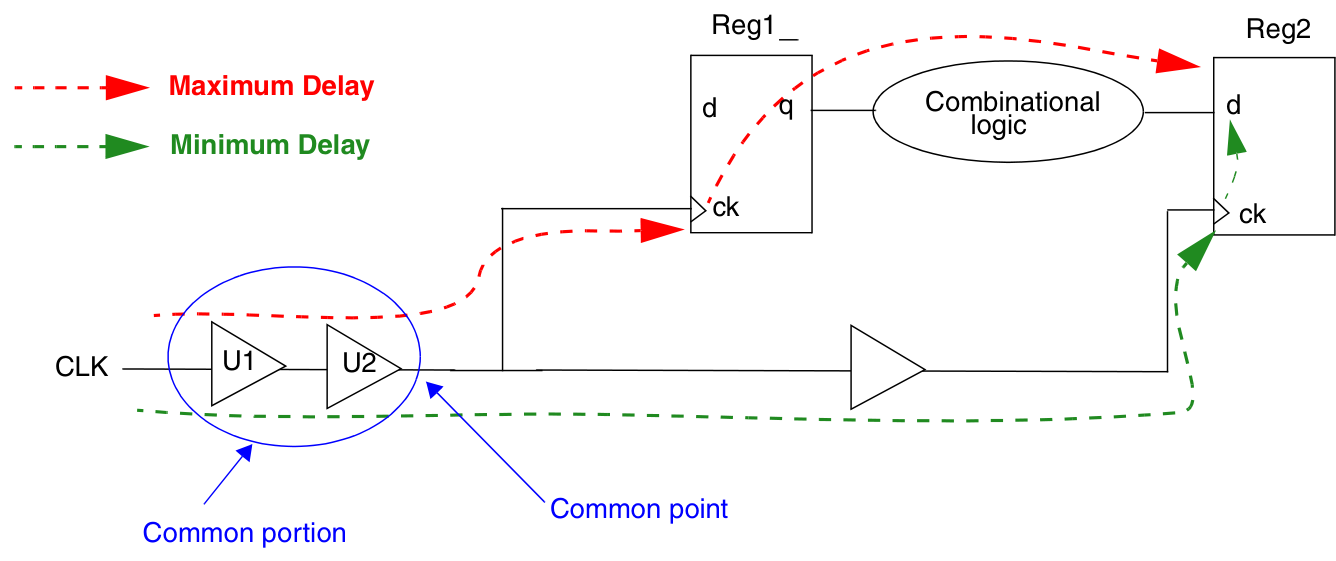
\includegraphics[width=0.9\textwidth]{fig-4-4.png}
  \caption{时钟再汇聚悲观量示例}
  \label{fig:crp}
\end{figure}

setup 分析时，对公共部分，工具对 launch 路径使用最大延迟、对 capture 路径使用最小延迟，从而产生时钟再汇聚悲观量。

从时钟源扇出到时序器件数据引脚、且 launch 与 capture 路径共享一段时钟路径的路径上，也可能引入悲观量，如图~\ref{fig:crp-fanout}。

\begin{figure}[htbp]
  \centering
  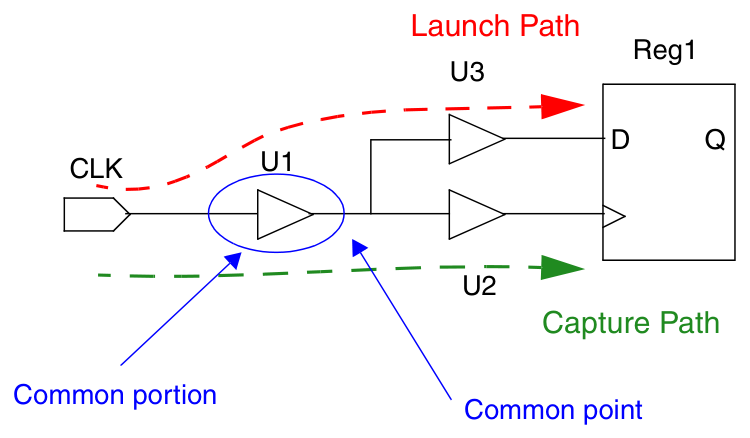
\includegraphics[width=0.72\textwidth]{fig-4-5.png}
  \caption{从时钟源扇出到数据引脚的时序路径}
  \label{fig:crp-fanout}
\end{figure}

\section{启用时钟再汇聚悲观量消除}
\subsection*{Enabling Clock Reconvergence Pessimism Removal}

把应用选项 \appopt{time.remove\_clock\_reconvergence\_pessimism} 设为 \cmd{true} 以启用 CRPR。默认值为 \cmd{false}，不执行 CRPR。

启用 CRPR 会使分析更不悲观，但会增加运行时间与内存占用。该变量的任何改变都会引起一次完整的时序更新。

还可以用下列应用选项进一步控制 CRPR：
\begin{itemize}
  \item 用 \appopt{time.clock\_reconvergence\_pessimism} 决定对公共部分上同极性或反极性的时钟跳变是否消除悲观量：
  \begin{itemize}
    \item \cmd{same\_transition}：仅当公共部分中的时钟跳变极性相同时才做 CRPR。
    \item \cmd{normal}：对公共部分中同极性与反极性的时钟跳变都做 CRPR。这是默认值。
  \end{itemize}
  \item 把 \appopt{time.crpr\_remove\_clock\_to\_data\_crp} 设为 \cmd{true}，消除 clock-to-data 路径与时钟路径之间的悲观量。默认值为 \cmd{false}。
\end{itemize}

\section{报告时钟再汇聚悲观量消除的计算}
\subsection*{Reporting Clock Reconvergence Pessimism Removal Calculations}

\cmd{report\_crpr} 报告两个寄存器时钟引脚或端口之间的 CRP 计算。需要指定 launch 与 capture 寄存器的引脚、时钟，以及检查类型（setup 或 hold）。例如：
\begin{lstlisting}
icc2_shell> report_crpr -from [get_pins ffa/CP] \
    -to [get_pins ffd/CP] -setup
\end{lstlisting}

该命令生成的报告给出：
\begin{itemize}
  \item 公共点的位置
  \item launch 与 capture 时钟边沿类型（上升或下降）
  \item 公共点处四个计算得到的到达时间（early 与 late，以及 rise 与 fall）
  \item 计算得到的 CRP 值（rise 与 fall）
  \item 用于 opening-edge 与 closing-edge 悲观量消除的值
\end{itemize}

\cmd{report\_crpr} 报告的 CRP 量可能与 \cmd{report\_timing} 略有不同。为提高计算效率，当相邻点之间的 CRP 差异过小时，\cmd{report\_timing} 会把多个点合并后再做 CRPR 计算。

% 第 5 章 Constraining Ports and Nets
\bichapter{约束端口与网线}{Constraining Ports and Nets}
\label{chap:ports}

时序分析与时序优化依赖于描述 block 中端口与网线特性的约束。本章说明这些约束及相关任务：
\begin{itemize}
  \item 指定输入端口与 inout 端口的驱动特性
  \item 为端口设置驱动单元
  \item 设置驱动电阻
  \item 设置输入转换时间
  \item 从端口去掉驱动特性
  \item 指定端口负载电容
  \item 理想网络简介
  \item 理想网络属性的传播
  \item 创建与删除理想网络
  \item 报告理想网络
  \item 检索理想对象
  \item 设置理想 latency 与理想转换时间
  \item 时序分析中忽略网线延迟
\end{itemize}

\section{指定输入端口与 inout 端口的驱动特性}
\subsection*{Specifying Drive Characteristics at Input and Inout Ports}

要约束输入或 inout 端口，应为它指定驱动电阻与输入转换时间，方法有两种：
\begin{itemize}
  \item 用 \cmd{set\_driving\_cell} 指定外部驱动单元。工具据此计算驱动电阻与输入转换时间。端口还会继承驱动单元的其他特性，例如设计规则约束。这是更准确的驱动特性表示。
  \item 用 \cmd{set\_drive} 与 \cmd{set\_input\_transition} 直接指定驱动电阻与输入转换时间。这是较不准确的表示。
\end{itemize}

若两种方法都用，由 \cmd{set\_driving\_cell} 所指定驱动单元导出的驱动电阻与输入转换时间，会替换 \cmd{set\_drive} 与 \cmd{set\_input\_transition} 指定的值。

用 \cmd{report\_ports -drive} 报告端口上的驱动单元，或驱动电阻与输入转换时间。

\section{为端口设置驱动单元}
\subsection*{Setting a Drive Driving Cell for Ports}

可以用 \cmd{set\_driving\_cell} 建模端口的外部驱动特性，从而约束输入或 inout 端口。工具使用驱动单元的时序弧来计算被约束端口的驱动特性。

必须指定：
\begin{itemize}
  \item 正在约束的端口。
  \item 用 \opt{-lib\_cell} 指定外部驱动器的库单元。使用该选项时，还要用 \opt{-library} 给出取得该单元的库名。若不指定库，工具从找到的第一个含有匹配单元的参考库中取得该单元。
\end{itemize}

还可以指定：
\begin{itemize}
  \item 用 \opt{-rise} 与 \opt{-fall} 为上升与下降转换分别指定驱动单元。默认同一个驱动单元同时用于两者。
  \item 用 \opt{-min} 与 \opt{-max} 为 early 与 late 分析分别指定驱动单元。默认同时用于两者。
  \item 用 \opt{-pin} 指定用来驱动端口的库单元输出引脚。若所指定的库单元有多个输出引脚且未使用该选项，工具随机挑选一个输出引脚来驱动被约束端口。
  \item 用 \opt{-from\_pin} 指定驱动单元的输入引脚，以选择用于计算驱动特性的时序弧。若不使用该选项，工具随机挑选驱动单元的一个输入引脚。
  \item 用 \opt{-input\_transition\_rise} 与 \opt{-input\_transition\_fall} 指定驱动单元输入端的上升与下降转换时间，用于计算驱动特性。默认驱动单元输入端的转换时间为零。
  \item 用 \opt{-dont\_scale} 要求工具不要按 block 的工作条件缩放驱动特性。默认会按工作条件缩放。
  \item 用 \opt{-no\_design\_rule} 要求不要把驱动单元的设计规则加到被约束端口上。默认会施加这些设计规则。
  \item 用 \opt{-multiply\_by} 给出一个乘数，乘到为被约束端口计算出的转换时间上。
\end{itemize}

对多 scenario 设计，所指定的驱动单元默认只作用于当前 scenario。还可以：
\begin{itemize}
  \item 用 \opt{-modes} 指定某些 mode 的全部 scenario。
  \item 用 \opt{-corners} 指定某些 corner 与当前 mode 的全部 scenario。
  \item 同时用 \opt{-modes} 与 \opt{-corners}。
  \item 用 \opt{-scenarios} 指定具体 scenario。使用该选项时不能再用 \opt{-modes} 或 \opt{-corners}。
\end{itemize}

下例用类型为 \cmd{AND2} 的库单元约束端口 \cmd{I2}，选择从其输入引脚 \cmd{A} 出发的时序弧，并把该输入引脚的上升与下降转换时间指定为 0.5：
\begin{lstlisting}
icc2_shell> set_driving_cell [get_ports I2] \
    -lib_cell AND2 -from_pin A \
    -input_transition_rise 0.5 -input_transition_fall 0.5
\end{lstlisting}

\begin{figure}[htbp]
  \centering
  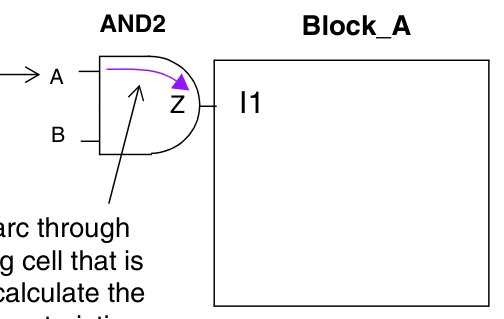
\includegraphics[width=0.72\textwidth]{fig-5-1.png}
  \caption{为驱动单元指定输入引脚与输入转换时间}
  \label{fig:drv-cell}
\end{figure}

\section{设置驱动电阻}
\subsection*{Setting Drive Resistance}

可以用 \cmd{set\_drive} 把外部驱动强度建模为一个电阻值，从而约束输入或 inout 端口。外部驱动器被建模为电源与该电阻串联。

必须指定正在约束的端口以及驱动电阻。还可以：
\begin{itemize}
  \item 用 \opt{-rise} 与 \opt{-fall} 为上升与下降分别指定驱动电阻。默认同时作用于两者。
  \item 用 \opt{-min} 与 \opt{-max} 为 early 与 late 分析分别指定驱动电阻。默认同时作用于两者。
\end{itemize}

对多 scenario 设计，驱动电阻默认只作用于当前 scenario。范围选项与 \cmd{set\_driving\_cell} 相同：\opt{-modes}、\opt{-corners}、两者同时，或 \opt{-scenarios}。

下例把端口 \cmd{A}、\cmd{B}、\cmd{C} 的上升与下降驱动电阻设为 2.0：
\begin{lstlisting}
icc2_shell> set_drive 2.0 {A B C}
\end{lstlisting}

\cmd{set\_driving\_cell} 是指定输入或 inout 端口驱动特性的更准确方法。若无法指定驱动单元，再用 \cmd{set\_drive} 与 \cmd{set\_input\_transition} 指定外部驱动特性。

\section{设置输入转换时间}
\subsection*{Setting an Input Transition Time}

用 \cmd{set\_input\_transition} 为输入或 inout 端口指定固定转换时间。端口的单元延迟为零。工具只在计算该端口所驱动逻辑的延迟时使用这个转换时间。

必须指定正在约束的端口以及输入转换时间。还可以：
\begin{itemize}
  \item 用 \opt{-rise} 与 \opt{-fall} 分别指定上升与下降输入转换时间。默认同时作用于两者。
  \item 用 \opt{-min} 与 \opt{-max} 分别指定 early 与 late 分析的输入转换时间。默认同时作用于两者。
  \item 用 \opt{-clock} 把输入转换时间相对某个时钟来指定。默认使用该时钟的上升沿。要使用下降沿，再加 \opt{-clock\_fall}。
\end{itemize}

对多 scenario 设计，输入转换时间默认只作用于当前 scenario。范围选项与前面相同。

下例把端口 \cmd{A}、\cmd{B}、\cmd{C} 的上升与下降输入转换时间设为 0.5：
\begin{lstlisting}
icc2_shell> set_input_transition 0.5 {A B C}
\end{lstlisting}

\section{从端口去掉驱动特性}
\subsection*{Removing Drive Characteristics From Ports}

表~\ref{tab:rm-drive} 中的命令从端口上去掉驱动信息。

\begin{table}[htbp]
\centering
\caption{去掉驱动信息的命令}
\label{tab:rm-drive}
\begin{tabularx}{\textwidth}{@{}X l@{}}
\toprule
要去掉的内容 & 使用的命令 \\
\midrule
一组端口上的驱动单元信息 & \cmd{remove\_driving\_cell} \\
驱动电阻 & \cmd{set\_drive 0.0} \\
输入转换时间 & \cmd{set\_input\_transition 0.0} \\
驱动数据以及全部用户指定数据，例如时钟、输入与输出延迟 & \cmd{reset\_design} \\
\bottomrule
\end{tabularx}
\end{table}

\section{指定端口负载电容}
\subsection*{Specifying Port Load Capacitance}

要准确做时序分析，工具需要连接到顶层端口的网线的外部负载电容，包括引脚电容与连线电容。可以用 \cmd{set\_load} 在端口上显式指定负载电容。

必须指定正在约束的端口以及电容值。还可以：
\begin{itemize}
  \item 用 \opt{-rise} 与 \opt{-fall} 分别为上升与下降指定电容。默认同时作用于两者。
  \item 用 \opt{-min} 与 \opt{-max} 分别为 early 与 late 分析指定电容。默认同时作用于两者。
  \item 用 \opt{-wire\_load} 把电容当作线负载；或同时用 \opt{-wire\_load} 与 \opt{-pin\_load}，既当作线负载也当作引脚负载。默认把电容当作引脚负载。
\end{itemize}

下例把全部输入上的电容设为 3.5，全部输出上的电容设为 5：
\begin{lstlisting}
icc2_shell> set_load 3.5 [all_inputs]
icc2_shell> set_load 5 [all_outputs]
\end{lstlisting}

\section{理想网络简介}
\subsection*{Introduction to Ideal Networks}

理想网络（ideal network）是一组免于时序更新、时序优化与 DRC 修复的单元、网线与引脚。理想网络中的对象忽略最大电容与转换时间设计规则。因此运行时间与时序优化都会改善。此外，优化期间工具不会去掉理想网络的源端口或叶级引脚。

例如，若把打算单独综合的某些高扇出网（如 scan-enable 与 reset）标为理想网，就可以避免优化期间不必要的 retiming 和不希望的设计改动，从而缩短运行时间。

指定理想网络的源端口或叶级引脚后，该源传递扇出中的网线、单元与引脚都被当作理想对象。理想对象具有下列性质：
\begin{itemize}
  \item 被标为 don't touch。
  \item 不受时序更新、延迟优化或 DRC 修复影响。
  \item 被赋予理想时序属性：理想 latency、理想转换时间，以及为零的理想电容。可用 \cmd{set\_ideal\_latency} 与 \cmd{set\_ideal\_transition} 分别修改 latency 与转换时间。
\end{itemize}

包含或驱动该源的单元会被设置 \cmd{size\_only} 属性。这保证 compile 期间理想网络的源不会丢失。

\section{理想网络属性的传播}
\subsection*{Propagation of the Ideal Network Property}

指定理想网络的源对象后，源对象传递扇出中的全部网线、单元与引脚都被当作理想对象。当前设计的任意输入端口或内部引脚都可以作为源对象，但层次边界上的引脚除外。

工具按一定传播规则，自动把理想网络属性扩散到源对象传递扇出中的网线、单元与引脚，并在到达下列位置时停止：
\begin{itemize}
  \item 时序单元。
  \item 不再有前向时序弧的点，例如输出端口或被禁用的时序弧。
  \item 不是理想对象的对象。
\end{itemize}

工具把下列对象视为理想对象：
\begin{itemize}
  \item 满足下列之一的引脚：出现在 \cmd{set\_ideal\_network} 的对象列表中；其单元为理想单元的驱动引脚；连接到理想网的负载引脚。
  \item 全部驱动引脚都是理想引脚的网线。
  \item 满足下列之一的组合单元：全部输入引脚都是理想的；一个输入引脚连接到常数网，且其余输入引脚都是理想的。带有 case analysis 属性的对象不当作常数。
\end{itemize}

若理想网络与时钟网络重叠，时钟时序信息（包括时钟 latency 与转换时间）覆盖重叠网络中时钟部分的理想时序。

对图~\ref{fig:ideal-net} 中的电路，假定把引脚 \cmd{U1/Z} 指定为理想网络的源。工具沿 \cmd{U1/Z} 传递扇出中的网线、单元与引脚传播理想网络属性，并停在名为 \cmd{REG1} 的时序单元处。工具还把 \cmd{dont\_touch} 属性传播到这些网线、单元与引脚，并在理想网络源的驱动器（单元 \cmd{IV1}）上设置 \cmd{size\_only}。

\begin{figure}[htbp]
  \centering
  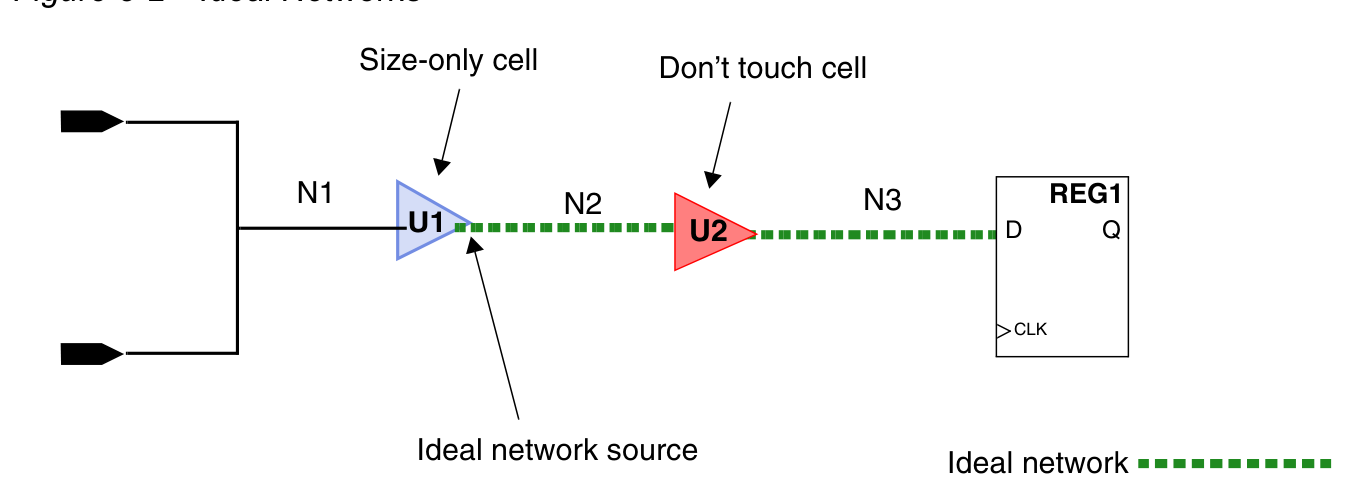
\includegraphics[width=0.9\textwidth]{fig-5-2.png}
  \caption{理想网络}
  \label{fig:ideal-net}
\end{figure}

\begin{figure}[htbp]
  \centering
  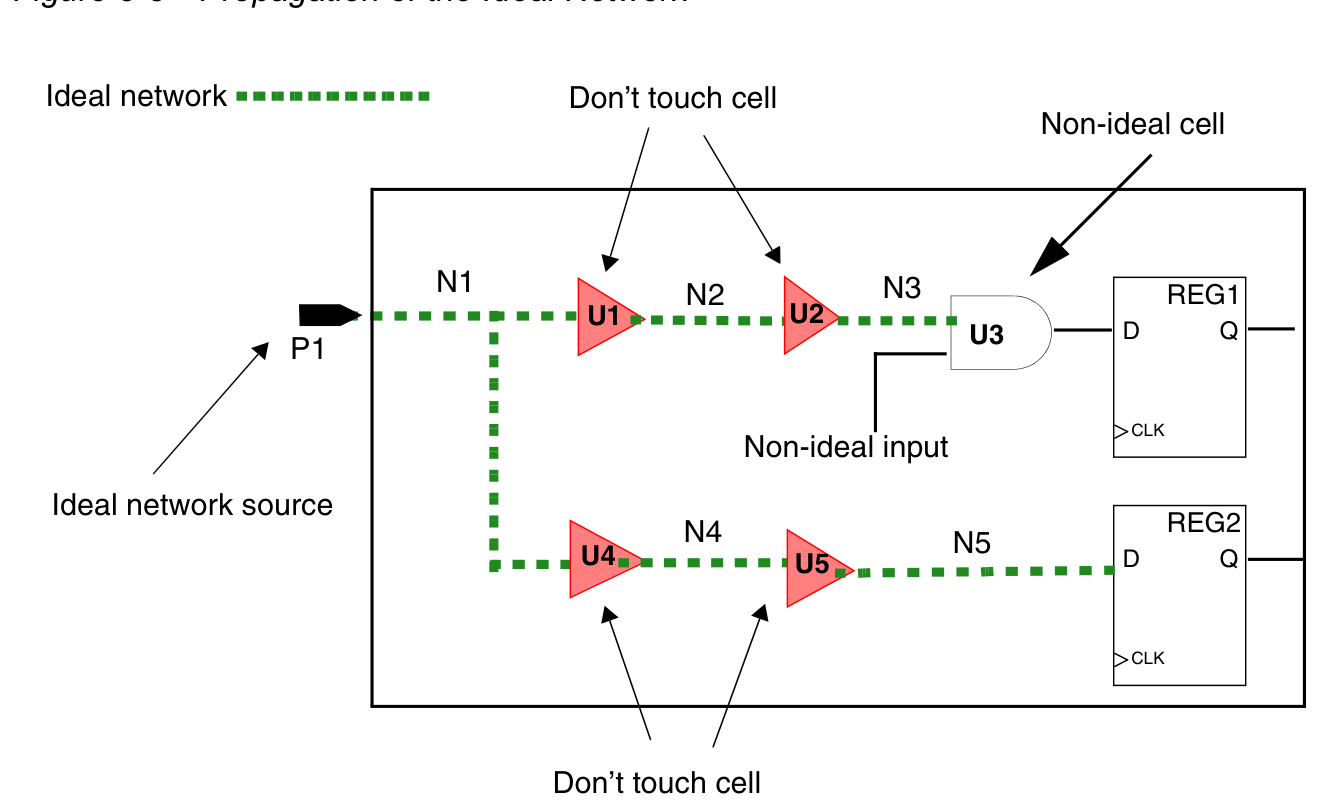
\includegraphics[width=0.9\textwidth]{fig-5-3.png}
  \caption{理想网络属性的传播}
  \label{fig:ideal-prop}
\end{figure}

\section{创建与删除理想网络}
\subsection*{Creating and Removing Ideal Networks}

用 \cmd{set\_ideal\_network} 创建理想网络。必须指定一组端口、引脚或网线作为理想网络的源。若指定的是网线，则该网的全局驱动引脚或端口被标为理想网络源。也就是说，理想网络属性加到所指定网线的全局驱动引脚或端口上。这样即使该网在优化中被去掉，理想网络属性也不会丢失。

用 \opt{-no\_propagate} 阻止理想网络穿过逻辑门继续传播。

下列命令把端口 \cmd{P1} 指定为理想网络的源：
\begin{lstlisting}
icc2_shell> set_ideal_network [get_ports P1]
\end{lstlisting}

用 \cmd{remove\_ideal\_network} 去掉理想网络设置，并把理想网络中的单元、网线与引脚恢复为非理想状态。

\section{报告理想网络}
\subsection*{Reporting Ideal Networks}

可用下列命令取得理想网络的更多信息：
\begin{itemize}
  \item \cmd{remove\_ideal\_network}：把理想网络中的单元、网线与引脚恢复到最初的非理想状态。
  \item \cmd{report\_attributes}：报告与单元、网线、引脚关联的属性。若用它报告理想网上的属性，会报告由 \cmd{set\_ideal\_network -no\_propagate} 设置的属性。
  \item \cmd{report\_nets}：报告网线信息；理想网以 ``I'' 标出。
\end{itemize}

\cmd{report\_timing}、\cmd{report\_cells} 与 \cmd{report\_nets} 会指出传播到理想网络非源对象上的理想网络属性，以及网络的源端口与源引脚。而 \cmd{report\_attributes} 与 \cmd{get\_attribute} 只对网络的源端口与源引脚显示理想网络属性，不显示已传播的属性。

\section{检索理想对象}
\subsection*{Retrieving Ideal Objects}

用下列命令检索理想对象：
\begin{itemize}
  \item \cmd{get\_nets -filter "ideal\_net == true"}：返回由 \cmd{set\_ideal\_network -no\_propagate} 设置的理想网。
  \item \cmd{get\_pins -filter "ideal\_network\_source == true"}：返回作为理想网络源的引脚。若再加过滤条件 \cmd{ideal\_network\_options == 1}，则只返回由 \cmd{set\_ideal\_network -no\_propagate} 设置的理想网络源引脚。
  \item \cmd{get\_ports -filter "ideal\_network\_source == true"}：返回作为理想网络源的端口。过滤条件 \cmd{ideal\_network\_options == 1} 的含义与引脚相同。
\end{itemize}

\section{设置理想 latency 与理想转换时间}
\subsection*{Setting Ideal Latency and Ideal Transition Time}

理想网络的默认 latency 与转换时间都是零。可用下列命令覆盖默认值：
\begin{itemize}
  \item \cmd{set\_ideal\_latency}
  \item \cmd{set\_ideal\_transition}
\end{itemize}

\begin{noteBox}
执行这两条命令中的任意一条时，理想网络的时序都会更新。
\end{noteBox}

这两条命令可以加在理想网或理想网络的源引脚上，也可以加在理想网络的任意非源引脚上。所指定的值覆盖库单元值或网线延迟值。对理想网络，理想 latency 与转换时间从源引脚传播到网络边界引脚。

理想网络中任意一点的总理想 latency，等于源引脚理想 latency 加上沿路径到达该点的各叶单元引脚理想 latency 之和。各源引脚与叶单元引脚上指定的理想转换时间彼此独立、不累积。未指定的输入引脚，其转换时间取最近一个已指定理想转换时间的引脚的值。该规则同样适用于边界引脚。

\cmd{set\_input\_delay} 适用于理想网络。该延迟被当作片外 latency 或 source latency。

用下列命令去掉理想 latency 与理想转换时间：
\begin{itemize}
  \item \cmd{remove\_ideal\_latency}
  \item \cmd{remove\_ideal\_transition}
\end{itemize}

\section{时序分析中忽略网线延迟}
\subsection*{Ignoring Net Delays During Timing Analysis}

默认情况下，IC Compiler II 在时序分析中同时考虑网线延迟与单元延迟。若要忽略网线延迟、只考虑单元延迟，把应用选项 \appopt{time.delay\_calculation\_style} 设为 \cmd{zero\_interconnect}，以启用零互连延迟计算。要把延迟计算风格恢复为默认，把该应用选项设为 \cmd{auto}。

% 第 6 章 Performing Parasitic Extraction
\bichapter{寄生参数提取}{Performing Parasitic Extraction}
\label{chap:extract}

准确的时序分析依赖于准确的网线 RC（寄生）信息。IC Compiler II 在布线前与布线后都能做 RC 提取，也可以反标详细的寄生参数。本章说明提取与寄生参数反标相关的任务：
\begin{itemize}
  \item 指定寄生工艺信息
  \item 指定提取用的寄生缩放因子
  \item 为详细布线网启用耦合电容提取
  \item 执行提取并生成寄生参数
  \item 执行设计内 signoff 提取
  \item 反标寄生参数
\end{itemize}

\section{指定寄生工艺信息}
\subsection*{Specifying the Parasitic Technology Information}

IC Compiler II 使用 TLUPlus 文件作为寄生工艺信息。TLUPlus 是存放各层 RC 系数的二进制表。

TLUPlus 模型把线宽、间距、密度与温度对电阻系数的影响包括进来，从而得到准确的 RC 提取结果。关于在互连工艺格式（Interconnect Technology Format，ITF）文件中建模这些效应，见 StarRC 文档。

做虚拟布线估计时，这一阶段尚未分配金属层，因此工具对分层 RC 系数做平均，以计算 RC 系数。

要把寄生信息关联到某个 corner，必须：
\begin{enumerate}
  \item 用 \cmd{read\_parasitic\_tech} 读入 TLUPlus 文件，并把它加到下列之一：
  \begin{itemize}
    \item 参考库。一般应把 TLUPlus 放在参考库中，使使用该工艺的全部 block 都能访问。
    \item 设计库。若参考库中没有 TLUPlus，则加到设计库。
  \end{itemize}
        可以读入一个或多个下列类型的 TLUPlus 文件：
  \begin{itemize}
    \item 仿真（emulation）TLUPlus，用于插入金属填充之前。
    \item 非仿真 TLUPlus，用于插入金属填充之后。
  \end{itemize}
        还必须用 \opt{-tlup} 指定 TLUPlus 文件。若给出相对路径或不给路径，工具用变量 \cmd{search\_path} 所定义的搜索路径定位文件。

        若 TLUPlus 中的层名与工艺文件中的层名不一致，必须在 TLUPlus 层映射文件中定义映射，语法见「TLUPlus 层映射文件」。用 \opt{-layermap} 指定层映射文件名。

        读入之后，TLUPlus 由其寄生工艺模型名标识。默认模型名是所指定 TLUPlus 文件的基本名，也可用 \opt{-name} 指定其他名称。

        例如，用名为 \cmd{my.layermap} 的层映射文件读入 \cmd{my.tlup}，并以寄生工艺模型名 \cmd{para1} 存入当前库：
\begin{lstlisting}
icc2_shell> read_parasitic_tech -tlup my.tlup \
    -layermap my.layermap -name para1
\end{lstlisting}
  \item 用 \cmd{set\_parasitic\_parameters} 把 TLUPlus 文件关联到 corner。
  \begin{itemize}
    \item 用 \opt{-corners} 关联到指定 corner。默认关联到当前 corner。
    \item 用 \opt{-early\_spec} 指定 early 延迟计算所用的 TLUPlus。
    \item 用 \opt{-early\_temperature} 指定 early 延迟计算所用的温度。
    \item 用 \opt{-late\_spec} 指定 late 延迟计算所用的 TLUPlus。
    \item 用 \opt{-late\_temperature} 指定 late 延迟计算所用的温度。
    \item 用 \opt{-library} 指定含有该寄生规格的库名。默认在当前库中查找 TLUPlus。
  \end{itemize}
        每个 corner 只能指定一个 early 和一个 late 寄生工艺模型。但可以在设计流程中随时更改，例如插入金属填充后改用非仿真 TLUPlus。

        \opt{-early\_spec} 与 \opt{-late\_spec} 使用 \cmd{read\_parasitic\_tech} 所赋的寄生工艺模型名。例如，让当前 corner 的 early 延迟计算使用模型名 \cmd{para1}：
\begin{lstlisting}
icc2_shell> set_parasitic_parameters -early_spec para1
\end{lstlisting}
\end{enumerate}

\subsection{TLUPlus 层映射文件}
\subsubsection*{TLUPlus Layer Mapping File}

TLUPlus 层映射文件使用下列语法：
\begin{lstlisting}
conducting_layers
tf_metal_layer_name1
ITF_metal_layer_name1
...
tf_metal_layer_namen
ITF_metal_layer_namen
via_layers
tf_via_layer_name1
ITF_via_layer_name1
...
tf_via_layer_namen
ITF_via_layer_namen
\end{lstlisting}

层映射文件中的注释行以星号（\cmd{*}）或井号（\cmd{\#}）开头。

\section{指定提取用的寄生缩放因子}
\subsection*{Specifying the Parasitic Scaling Factors for Extraction}

寄生缩放因子用来按特定条件调整电阻与电容，例如最小或最大延迟计算，以及虚拟布线或详细布线的网线。默认缩放因子为 1.0，工具不调整电阻与电容。

用 \cmd{set\_extraction\_options} 指定寄生缩放因子。默认作用于当前 corner。用 \opt{-corners} 作用于指定 corner。这些因子在用 \cmd{save\_block} 把 block 存入设计库时一并保存。

表~\ref{tab:ext-scale} 给出设置各种寄生缩放因子所用的选项。

\begin{table}[htbp]
\centering
\caption{设置寄生缩放因子的选项}
\label{tab:ext-scale}
\begin{tabularx}{\textwidth}{@{}X l@{}}
\toprule
寄生量 & 选项 \\
\midrule
详细布线电阻 & \cmd{-late\_res\_scale}、\cmd{-early\_res\_scale} \\
详细布线电容 & \cmd{-late\_cap\_scale}、\cmd{-early\_cap\_scale} \\
详细布线耦合电容 & \cmd{-late\_ccap\_scale}、\cmd{-early\_ccap\_scale} \\
虚拟布线水平电阻 & \cmd{-late\_vr\_horizontal\_res\_scale}、\cmd{-early\_vr\_horizontal\_res\_scale} \\
虚拟布线垂直电阻 & \cmd{-late\_vr\_vertical\_res\_scale}、\cmd{-early\_vr\_vertical\_res\_scale} \\
虚拟布线通孔电阻 & \cmd{-late\_vr\_via\_res\_scale}、\cmd{-early\_vr\_via\_res\_scale} \\
虚拟布线水平电容 & \cmd{-late\_vr\_horizontal\_cap\_scale}、\cmd{-early\_vr\_horizontal\_cap\_scale} \\
虚拟布线垂直电容 & \cmd{-late\_vr\_vertical\_cap\_scale}、\cmd{-early\_vr\_vertical\_cap\_scale} \\
\bottomrule
\end{tabularx}
\end{table}

例如，把当前 corner 最大延迟计算所用的电容增大 10\%，把最小延迟计算所用的电容减小 5\%：
\begin{lstlisting}
icc2_shell> set_extraction_options \
    -late_cap_scale 1.1 -early_cap_scale 0.95
\end{lstlisting}

用 \cmd{report\_extraction\_options} 报告寄生缩放因子。默认报告全部 corner；用 \opt{-corners} 报告指定 corner。

要把某个寄生缩放因子复位，用 \cmd{set\_extraction\_options} 把它设回 1.0。

\section{为详细布线网启用耦合电容提取}
\subsection*{Enabling Coupling Capacitance Extraction for Detailed Routed Nets}

默认情况下，对已详细布线的 block 做提取时，工具不单独提取网与网之间的耦合电容。耦合效应包含在总电容中。

要为详细布线网提取耦合电容，把应用选项 \appopt{extract.enable\_coupling\_cap} 设为 \cmd{true}：
\begin{lstlisting}
icc2_shell> set_app_options -name extract.enable_coupling_cap \
    -value true
\end{lstlisting}

\section{执行提取并生成寄生参数}
\subsection*{Performing Extraction and Generating Parasitics}

工具在更新时序信息时自动做提取。可以显式运行 \cmd{update\_timing} 来更新时序并执行提取。要用 SPEF 格式写出提取到的寄生参数，使用 \cmd{write\_parasitics}。

使用 \cmd{write\_parasitics} 时必须用 \opt{-output} 指定输出文件名。工具为每个 corner 生成一个 SPEF 文件。这些文件名由所给输出文件名，以及工艺名、温度和 \cmd{set\_extraction\_options} 指定的缩放因子导出。工具还会生成名为 \cmd{XX.spef\_scenario} 的文件，列出每个输出 SPEF 所关联的 scenario。

默认情况下，\cmd{write\_parasitics}：
\begin{itemize}
  \item 把网名映射为数字，写网线寄生信息时使用这些数字，以减小文件。要用原网名，使用 \opt{-no\_name\_mapping}。
  \item 为顶层设计生成一个 SPEF。要为每个下层 block 分别生成 SPEF，使用 \opt{-hier}。
\end{itemize}

运行 \cmd{write\_parasitics} 时，若寄生信息已过时，工具会执行提取。但若使用 \opt{-hier}，工具不检查下层 block 是否已经提取。因此在带 \opt{-hier} 使用 \cmd{write\_parasitics} 之前，应先运行 \cmd{update\_timing}。

\section{执行设计内 signoff 提取}
\subsection*{Performing In-Design Signoff Extraction}

IC Compiler II 支持在已布线设计上使用 StarRC 提取能力做设计内（In-Design）signoff 提取。该功能改善与 StarRC 的相关性，并可与 PrimeTime 延迟计算配合，改善布线后 QoR。由于运行较慢，StarRC 设计内提取应只在设计收敛的最后阶段使用。

在运行 \cmd{route\_opt} 之前，按下列步骤使用 StarRC 设计内提取：
\begin{enumerate}
  \item 用 \cmd{set\_starrc\_in\_design -config} 指定运行 StarRC 提取的配置文件。配置文件必须包含：
  \begin{itemize}
    \item \cmd{SIGNOFF\_IMAGE}：StarRC 可执行文件的位置。
    \item \cmd{CORNER\_GRD\_FILE}：列出每个 corner 及对应 StarRC nxtgrd 文件的文件。
    \item 下列设置之一：
    \begin{itemize}
      \item \cmd{MAPPING\_FILE}：StarRC 层映射文件（推荐）。
      \item \cmd{COMMAND\_FILE}：StarRC 命令文件。若 StarRC 命令文件中的设置与 IC Compiler II 冲突，工具使用 IC Compiler II 的设置。例如，\cmd{set\_extraction\_options} 指定的耦合电容阈值为 1.0~fF，而 StarRC 命令文件把 \cmd{COUPLING\_ABS\_THRESHOLD} 设为 0.5~fF，则设计内提取使用 1.0~fF。
    \end{itemize}
  \end{itemize}
        配置文件示例：
\begin{lstlisting}
SIGNOFF_IMAGE: /home/star_rcxt_2016.06/bin/StarXtract
CORNER_GRD_FILE: corner_grd.mapping
MAPPING_FILE: star.mapping
\end{lstlisting}
  \item （可选）用 \cmd{report\_starrc\_in\_design} 报告 StarRC 设计内提取的设置。
  \item 用下列应用选项启用 StarRC 设计内提取：
\begin{lstlisting}
icc2_shell> set_app_options -list {extract.starrc_mode true}
\end{lstlisting}
\end{enumerate}

\begin{noteBox}
若设计尚未布线，即使该应用选项为 \cmd{true}，也不会执行 StarRC 设计内提取。
\end{noteBox}

要使用 StarRC 提取得到的寄生信息，在运行 \cmd{report\_timing}、\cmd{report\_qor} 或 \cmd{write\_parasitics} 之前，先运行 \cmd{update\_timing -full}。

\section{反标寄生参数}
\subsection*{Back-Annotating Parasitics}

可以读入外部工具以 SPEF 格式生成的网线寄生数据，并在时序分析的延迟计算中使用。用 \cmd{read\_parasitics}，并以 \opt{-corner\_spef} 一次或多次为每个 corner 指定一个 SPEF 文件。若多个 corner 共用同一个 SPEF，可以在一次 \opt{-corner\_spef} 中列出多个 corner。

默认把 SPEF 中的寄生参数加到顶层 block。要为下层 block 读入 SPEF，使用 \opt{-block}。使用该选项时，\opt{-corner\_spef} 中的 corner 必须在顶层定义。

下例：
\begin{itemize}
  \item 在顶层，corner \cmd{C1}、\cmd{C2} 使用 \cmd{TOP\_C1C2.spef}，corner \cmd{C3}、\cmd{C4} 使用 \cmd{TOP\_C3C4.spef}。
  \item 在 block 级，corner \cmd{C1}、\cmd{C2} 使用 \cmd{BLK\_C1C2.spef}，corner \cmd{C3}、\cmd{C4} 使用 \cmd{BLK\_C3C4.spef}。
\end{itemize}
\begin{lstlisting}
icc2_shell> read_parasitics -corner_spef {{C1 C2} TOP_C1C2.spef} \
    -corner_spef {{C3 C4} TOP_C3C4.spef}
icc2_shell> read_parasitics -block BLK \
    -corner_spef {{C1 C2} BLK_C1C2.spef} \
    -corner_spef {{C3 C4} BLK_C3C4.spef}
\end{lstlisting}

\cmd{read\_parasitics} 执行后，工具打印未被反标的网线数量，并对 SPEF 未反标的网线执行提取。

% 第 7 章 Generating Reports
\bichapter{生成报告}{Generating Reports}
\label{chap:reports}

IC Compiler II 可以生成关于设计内容与分析结果的多种报告。本章说明最常用的报告：
\begin{itemize}
  \item 控制延迟计算
  \item 报告时序路径
  \item 报告逻辑 DRC 违例
  \item 报告 QoR
  \item 生成并分析 QoR 快照
  \item 报告时序弧的延迟
  \item 报告引脚或端口上的时钟或数据到达时间
  \item 检查时序约束与设置
  \item 检查时序分析或提取设置的一致性
  \item 分析 IC Compiler II 与 PrimeTime 之间的时序相关性
\end{itemize}

\section{控制延迟计算}
\subsection*{Controlling Delay Calculation}

IC Compiler II 同时支持 Elmore 与 Arnoldi 延迟计算模型。不能指定使用哪一种；工具根据设计状态选择最合适的模型。

时序分析中若要忽略网线延迟，使用下列应用选项：
\begin{lstlisting}
icc2_shell> set_app_options -name time.delay_calculation_style \
    -value zero_interconnect
\end{lstlisting}

\subsection{使用 PrimeTime 延迟计算引擎}
\subsubsection*{Using the PrimeTime Delay Calculation Engine}

设计布线之后，可以用下列应用选项在时序分析与布线后优化中启用 PrimeTime 延迟计算引擎：
\begin{lstlisting}
icc2_shell> set_app_options -name time.use_pt_delay -value true
\end{lstlisting}

使用 PrimeTime 延迟计算引擎时，除 \cmd{.ndm} 文件外，还需要参考库的 \cmd{.db} 文件。若创建参考库之后 \cmd{.db} 的位置已改变，把新位置加入 \cmd{search\_path}，例如：
\begin{lstlisting}
icc2_shell> lappend search_path /libraries/ref_libs/db_files
\end{lstlisting}

关于在 \cmd{route\_opt} 布线后优化中使用 PrimeTime 延迟计算引擎的更多信息，见 \textit{IC Compiler II Implementation User Guide}。

\section{报告时序路径}
\subsection*{Reporting Timing Paths}

用 \cmd{report\_timing} 报告 block 中的时序路径。默认报告当前 block 上已启用 setup 分析的全部 scenario 中，最大（setup）延迟最差的那条路径。要报告最小（hold）延迟分析，使用 \opt{-delay\_type}。

还可以：
\begin{itemize}
  \item 用 \opt{-modes} 报告与指定 mode 关联的全部 scenario。
  \item 用 \opt{-corners} 报告与指定 corner 关联的全部 scenario。
  \item 用 \opt{-scenarios} 报告指定 scenario。
\end{itemize}

要报告某个 scenario 的最大与最小时序信息，必须为该 scenario 启用 setup 与 hold 分析。

还可以把报告进一步限制为：
\begin{itemize}
  \item 用 \opt{-groups} 只包含指定 path group。
  \item 只包含满足下列条件的路径：
  \begin{itemize}
    \item 用 \opt{-from}、\opt{-rise\_from} 或 \opt{-fall\_from} 从指定点出发。
    \item 用 \opt{-to}、\opt{-rise\_to} 或 \opt{-fall\_to} 结束于指定点。
    \item 用 \opt{-through}、\opt{-rise\_through} 或 \opt{-fall\_through} 经过指定点。
    \item 用 \opt{-start\_end\_pair} 位于指定起点与终点对之间。
  \end{itemize}
  \item 用 \opt{-max\_paths} 或 \opt{-nworst} 只包含指定条数的路径，或每个终点指定条数的路径。
  \item 用 \opt{-slack\_lesser\_than} 只包含 slack 小于指定值的路径。
  \item 排除下列时序路径：
  \begin{itemize}
    \item 用 \opt{-exclude} 排除从、经过或到达指定 pin、port、net 或单元实例的路径。
    \item 用 \opt{-rise\_exclude} 排除在这些对象上为上升沿的路径。
    \item 用 \opt{-fall\_exclude} 排除在这些对象上为下降沿的路径。
  \end{itemize}
\end{itemize}

用下列选项控制打印的路径或对象信息：
\begin{itemize}
  \item \opt{-nets}：包含网线。
  \item \opt{-physical}：包含引脚位置。
  \item \opt{-attributes}：包含属性。
  \item \opt{-input\_pins}：包含输入引脚。
  \item \opt{-include\_hierarchical\_pins}：包含层次引脚。
  \item \opt{-transition\_time}：包含转换时间。
  \item \opt{-capacitance}：包含电容。
  \item \opt{-exception}：包含作用于所打印每条时序路径的主导时序例外（false path、multicycle path，以及最小与最大延迟）。包含例外信息会增加运行时间。
  \item \opt{-process}、\opt{-voltage}、\opt{-temperature}：包含工作条件的工艺、电压与温度。
  \item \opt{-derate}：包含时序 derate。
  \item \opt{-crosstalk\_delta}：在启用信号完整性时包含串扰信息。
  \item \opt{-variation}：在启用 POCV 时，包含每个路径元素统计时间增量的均值与标准差。还可用应用选项 \appopt{time.pocvm\_use\_normalized\_reporting} 进一步控制该变异信息，详见其 man 页。
  \item \opt{-skip\_transparency\_window}：对基于锁存器的设计，不打印透明窗口。
\end{itemize}

还可以这样控制报告格式：
\begin{itemize}
  \item 用 \opt{-path\_type} 指定路径报告风格，例如完整路径、只报告终点等。
  \item 用 \opt{-report\_by} 按 mode、corner、scenario、path group 或整个 block 组织报告。
  \item 用 \opt{-sort\_by} 按路径、path group 或 slack 排序。
  \item 用 \opt{-significant\_digits} 指定显示的有效数字位数。
  \item 用 \opt{-nosplit} 在列溢出时避免拆行。
\end{itemize}

下面是 \cmd{report\_timing} 默认输出的示例。

\begin{lstlisting}[caption={report\_timing 报告示例}]
icc2_shell> report_timing
****************************************
Report : timing
        -path_type full
        -delay_type max
        -nworst 1
        -max_paths 1
        -report_by design
Design : my_design
****************************************
 Startpoint: u0_3/p0/mul0/m0_U1_INT_SUMR_reg_1_/CLK
             (rising edge-triggered flip-flop)
 Endpoint: u0_3/p0/iu0/r_reg_E__OP2__31_/D
             (rising edge-triggered flip-flop)
 Mode: my_mode
 Corner: wc_corner
 Scenario: wc_scenario
 Path Group: pci_clk
 Path Type: max
 Launch clock: pci_clk  r
 Capture clock: pci_clk  r
  Point                                    Fanout  Cap   Trans  Incr   Path
--------------------------------------------------------------------------------
  clock pci_clk (rise edge)                                   0.00   0.00
  clock network delay (ideal)                                 2.00   2.00
  .../CLK (SDFFX1_LVT)                                0.00  0.00   2.00 r
  .../QN (SDFFX1_LVT)                          1      7.19  0.11  0.18   2.18 f
  ...
  data arrival time                                                  6.37
  clock pci_clk (rise edge)                                   5.00   5.00
  clock network delay (ideal)                                 2.00   7.00
  clock uncertainty                                          -0.40   6.60
  library setup time                                         -0.20   6.40
  data required time                                                 6.40
--------------------------------------------------------------------------------
  slack (MET)                                                        0.03
\end{lstlisting}

\subsection{控制时序报告中的列顺序}
\subsubsection*{Controlling the Column Order in a Timing Report}

默认报告给出起点、终点、path group、路径类型、数据路径与时钟路径上的增量延迟与累积延迟、路径终点的数据要求时间，以及该路径的时序 slack。

用应用选项 \appopt{time.report\_timing\_column\_order} 控制列顺序，例如：
\begin{lstlisting}
icc2_shell> set_app_options -name time.report_timing_column_order \
    -value {point incr path cap fanout trans}
\end{lstlisting}

该应用选项的合法值为 \cmd{point}、\cmd{incr}、\cmd{path}、\cmd{cap}、\cmd{fanout}、\cmd{trans}、\cmd{derate}、\cmd{mean} 与 \cmd{sensit}。

\subsection{报告无约束时序路径}
\subsubsection*{Reporting Unconstrained Timing Paths}

默认情况下，\cmd{report\_timing} 与 \cmd{get\_timing\_paths} 不报告无约束的时序路径。要报告它们，在运行这两条命令之前设置：
\begin{lstlisting}
icc2_shell> set_app_options -list {time.report_unconstrained_paths true}
\end{lstlisting}

无约束路径的 slack 为无穷大，只能用路径过滤来报告，例如：
\begin{lstlisting}
icc2_shell> report_timing [filter_collection \
    [get_timing_paths -max_paths 200000 -to [all_outputs]] \
    slack=="INFINITY"]
\end{lstlisting}

\section{报告逻辑 DRC 违例}
\subsection*{Reporting the Logical DRC Violations}

用 \cmd{report\_constraints} 报告逻辑 DRC 违例。该命令显示 block 中约束违例的摘要，包括违例量、最差违例对象的信息，以及违例的加权代价。

默认检查下列时序约束：
\begin{itemize}
  \item 最小路径延迟：包括寄存器或带输出延迟的端口上的 hold 违例，以及 \cmd{set\_min\_delay} 的违例。
  \item 最大路径延迟：包括寄存器或带输出延迟的端口上的 setup 违例，以及 \cmd{set\_max\_delay} 的违例。
  \item 最大转换时间。
  \item 最大电容。
  \item 最小电容。
\end{itemize}

用下列选项把报告限制到某一种约束：\opt{-min\_delay}、\opt{-max\_delay}、\opt{-max\_transition}、\opt{-max\_capacitance}、\opt{-min\_capacitance}。

默认只显示当前 block 中每种约束的最差违例以及总代价。要报告全部违例而不仅是最差违例，使用 \opt{-all\_violators}。

下面是默认输出的节选。
\begin{lstlisting}[caption={默认约束报告}]
icc2_shell> report_constraints
    Group (min_delay/hold)       Cost     Weight     Cost     Scenario
    pci_clk                      0.00      1.00      0.00  wc_scenario
    pci_clk                      1.12      1.00      1.12  bc_scenario
    min_delay/hold                                   1.13
    Group (max_delay/setup)      Cost     Weight     Cost     Scenario
    pci_clk                      0.44      1.00      0.44  wc_scenario
    max_delay/setup                                  0.68
    Constraint                                       Cost
    min_delay/hold                                   1.13  (VIOLATED)
    max_delay/setup                                  0.68  (VIOLATED)
    max_transition                                 417.69  (VIOLATED)
    max_capacitance                              189895.48  (VIOLATED)
    min_capacitance                                100.52  (VIOLATED)
\end{lstlisting}

\section{报告 QoR}
\subsection*{Reporting the QoR}

用 \cmd{report\_qor} 生成 block 的结果质量（quality of results，QoR）及其他统计摘要。它报告时序 path group 细节、单元数量，以及当前 block 的统计，包括组合面积、非组合面积与总面积。该命令还报告静态功耗与设计规则违例。

默认报告全部 active scenario 的 QoR。还可以：
\begin{itemize}
  \item 用 \opt{-modes} 报告与指定 mode 关联的全部 scenario。
  \item 用 \opt{-corners} 报告与指定 corner 关联的全部 scenario。
  \item 用 \opt{-scenarios} 报告指定 scenario。
\end{itemize}

下面是 \cmd{report\_qor} 报告的节选。
\begin{lstlisting}[caption={report\_qor 报告示例}]
icc2_shell> report_qor
Information: Design Average RC value per unit length: (NEX-011)
Information: r = 1.792938 ohm/um, c = 0.079907 ff/um (X dir)
Scenario           'bc_scenario'
Timing Path Group  'pci_clk'
Worst Hold Violation:             -0.15
Total Hold Violation:             -8.79
No. of Hold Violations:             283
Scenario           'wc_scenario'
Timing Path Group  'pci_clk'
Levels of Logic:                     55
Critical Path Length:              2.79
Critical Path Slack:               0.03
Critical Path Clk Period:          3.00
Total Negative Slack:              0.00
No. of Violating Paths:               0
Cell Count
Hierarchical Cell Count:            694
Leaf Cell Count:                 116919
Buf/Inv Cell Count:               17031
Area
Combinational Area:          8365846.92
Noncombinational Area:        571218.74
Cell Area:                   8937065.66
Design Rules
Total Number of Nets:            142890
Nets with Violations:               273
Max Trans Violations:                12
Max Cap Violations:                 262
\end{lstlisting}

在 Cell Count 一节中，报告给出 block 中的宏单元数量。要算作宏单元，单元不能是层次单元，且其库单元上必须设置了 \cmd{is\_macro\_cell} 属性。

\section{生成并分析 QoR 快照}
\subsection*{Generating and Analyzing a QoR Snapshot}

用 \cmd{create\_qor\_snapshot} 生成设计 QoR 的详细信息。该命令从时序、设计规则、面积与功耗几方面度量并报告设计质量，并把质量信息存入一组快照文件。

随后可以：
\begin{itemize}
  \item 用 \cmd{report\_qor\_snapshot} 取出并报告快照中的 QoR 信息。
  \item 用 \cmd{query\_qor\_snapshot} 有选择地取出、排序并显示快照中所需的信息。
  \item 用 \cmd{remove\_qor\_snapshot} 删除快照。
\end{itemize}

用 \cmd{create\_qor\_snapshot} 创建快照时，必须用 \opt{-name} 指定名称。报告、查询或删除快照时使用该名称。

默认对 block 的全部 scenario 创建 QoR 快照。要为指定 scenario 创建，使用 \opt{-scenarios}，例如：
\begin{lstlisting}
icc2_shell> create_qor_snapshot -name func1 -scenarios func1
\end{lstlisting}

报告节选如下。它给出各时序组的 WNS、setup / hold 的 WNS 与 TNS、违例条数、最大转换与最大电容违例、面积、单元数、缓冲器/反相器数量、标准单元利用率、CPU 时间与内存，以及 slack 直方图。
\begin{lstlisting}
No. of scenario = 1
s1 = func1
WNS of each timing group:                       s1
SD_DDR_CLK                                    1.07
PCI_CLK                                      -1.76
Setup WNS:                                   -1.76
Setup TNS:                                 -102.47
Number of setup violations:                     95
Hold WNS:                                    -0.50
Number of max cap violations:                   28
Area:                                   444776.034
Cell count:                                  53399
Histogram:             s1
Max violations:        95
   above ~ -0.7  ---   40
    -0.6 ~ -0.7  ---   55
\end{lstlisting}

默认把快照存在当前工作目录下名为 \cmd{snapshot} 的目录中。要指定其他位置，使用应用选项 \appopt{time.snapshot\_storage\_location}。

用 \cmd{create\_qor\_snapshot}、\cmd{report\_qor\_snapshot} 或 \cmd{query\_qor\_snapshot} 创建、报告或查询快照时，可用 \opt{-display} 在 GUI 中显示结果。

下例分析快照，并显示最差负 slack 介于 $-2.0$ 与 $-1.0$ 之间的路径：
\begin{lstlisting}
icc2_shell> query_qor_snapshot -name func1 -display \
    -filters "-wns -2.0,-1.0"
\end{lstlisting}

下例显示逻辑级数超过 10 的路径：
\begin{lstlisting}
icc2_shell> query_qor_snapshot -name func1 -display \
    -filters "-logic_level 10, "
\end{lstlisting}

\section{报告时序弧的延迟}
\subsection*{Reporting the Delay of a Timing Arc}

用 \cmd{report\_delay\_calculation} 取得时序路径上某条单元或网线时序弧的延迟计算详细报告。

用 \opt{-from} 与 \opt{-to} 指定单元或网线的 ``from'' 与 ``to'' 引脚。这两个引脚可以是单元的输入与输出，以报告单元延迟；也可以是网线的驱动引脚与负载引脚，以报告网线延迟。

默认报告当前 scenario 的延迟计算。可用 \opt{-mode} 与 \opt{-corner} 指定要报告的 mode 与 corner，或用 \opt{-scenario} 指定 scenario。

下面是当前 scenario 的报告节选。
\begin{lstlisting}[caption={延迟计算报告}]
icc2_shell> report_delay_calculation \
    -from u0_3/p0/mul0/m0_U1_INT_SUMR_reg_1_/CLK \
    -to u0_3/p0/mul0/m0_U1_INT_SUMR_reg_1_/QN
cap units: 1.00fF  res units: 1.00MOhm  time units: 1.00ns
Current delay calculation style: auto
Current min Elmore tau: 0.00s
Current min Arnoldi tau: 2.00ps
Cell arc:
Cell: .../m0_U1_INT_SUMR_reg_1_ (FD1_LVT)
From-pin: CLK  To-pin: QN
Sense:   rising_edge
            Input                  Output  Stored   Stored        Delay
            slew    Load   Delay   slew    delay    output slew   derate
early rise: 0.29    7.27   0.22    0.11    0.22     0.11          0.99
 late rise: 0.29    7.27   0.22    0.11    0.22     0.11          1.01
early fall: 0.29    6.85   0.20    0.10    0.20     0.10          0.99
 late fall: 0.29    6.85   0.20    0.10    0.20     0.10          1.01
\end{lstlisting}

\section{报告引脚或端口上的时钟或数据到达时间}
\subsection*{Reporting the Clock or Data Arrival Time at Pins or Ports}

要取得数据网上某个 pin 或 port 处数据信号的到达时间，用 \cmd{get\_attribute} 查询 \cmd{arrival\_window} 属性：
\begin{lstlisting}
icc2_shell> get_attribute [get_pins U50/Y] arrival_window
{{{SYS_CLK} pos_edge {min_r_f 0.367955 0.361167} {max_r_f 0.385574 0.383949}}}
\end{lstlisting}

对到达窗口，工具报告时钟名、发射该路径的边沿类型，以及该引脚上最小与最大的上升、下降到达时间。若多个时钟发射的数据到达同一引脚，工具为每个时钟发射的数据分别报告一个到达窗口。

要取得时钟网络上某个 pin 或 port 处时钟信号的到达时间，查询 \cmd{clock\_arrival\_window}：
\begin{lstlisting}
icc2_shell> get_attribute [get_pins CT_BUF_7/Y] clock_arrival_window
{{{SYS_CLK} pos_edge {min_r_f 1.03046 --} {max_r_f 1.03067 --}}}
\end{lstlisting}

对时钟到达窗口，工具报告时钟名、有效边沿类型，以及按该有效边沿在时钟引脚上的最小与最大上升或下降到达时间。若多个时钟或同一时钟的多个有效边沿到达该引脚，工具为每个时钟或时钟边沿分别报告一个到达窗口。

\section{检查时序约束与设置}
\subsection*{Checking the Timing Constraints and Settings}

约束不正确的路径可能不会出现在违例报告中，从而漏掉有违例的路径。用 \cmd{check\_timing} 检查指定错误或缺失的约束以及其他时序问题。

表~\ref{tab:check-timing} 列出 \cmd{check\_timing} 所做的检查。
\begin{itemize}
  \item 用 \opt{-all} 执行全部检查。
  \item 用 \opt{-include} 在默认检查之外再包含指定检查。
  \item 用 \opt{-exclude} 从默认检查中排除指定检查。
\end{itemize}

默认对全部 active scenario 做时序检查。还可以用 \opt{-modes}、\opt{-corners} 或 \opt{-scenarios} 限定范围。

\begin{table}[htbp]
\centering
\caption{\cmd{check\_timing} 所执行的检查类型}
\label{tab:check-timing}
\begin{tabularx}{\textwidth}{@{}l c X@{}}
\toprule
检查类型 & 默认 & 工具的行为 \\
\midrule
\cmd{gated\_clock} & 是 &
对任何没有到达寄存器时钟引脚的门控时钟发出警告。 \\
\cmd{generated\_clock} & 是 &
检查生成时钟网络，并在下列情况下发出警告：生成时钟没有到达 master 时钟的路径；没有满足所指定极性关系的路径；多个生成时钟形成环路；生成时钟未被展开；生成时钟没有指定周期。 \\
\cmd{loops} & 是 &
发现组合反馈环时发出警告。 \\
\cmd{no\_clock} & 是 &
没有时钟到达寄存器时钟引脚时发出警告。 \\
\cmd{no\_input\_delay} & 是 &
输入端口没有指定与时钟相关的延迟时发出警告。 \\
\cmd{unconstrained\_endpoints} & 是 &
寄存器数据引脚或主输出无约束时发出警告。 \\
\cmd{clock\_crossing} & 否 &
时序路径跨越时钟域时发出警告。 \\
\cmd{data\_check} & 否 &
没有时钟信号或多个时钟信号到达 data check 寄存器的参考引脚时发出警告。 \\
\cmd{multiple\_clock} & 否 &
多个时钟到达寄存器引脚时发出信息消息。 \\
\bottomrule
\end{tabularx}
\end{table}

下面是 \cmd{check\_timing} 的输出示例。
\begin{lstlisting}
icc2_shell> check_timing
Warning: The register clock pin 'F1/CLK' has no fanin clocks. (TCK-002)
Warning: The reported endpoint 'OUT' is unconstrained. Reason: 'no check'. (TCK-001)
Warning: The reported endpoint 'F1/DATA' is unconstrained. Reason: 'unclocked'. (TCK-001)
\end{lstlisting}

也可以用 \cmd{check\_design -checks timing} 做时序检查：
\begin{lstlisting}
icc2_shell> check_design -checks timing
Running atomic-check 'timing'
Rule    Type   Count Message
TCK-002  Warn   3      The register clock pin '%pin' has no fanin clocks.
Total 7 EMS messages : 0 errors, 3 warnings, 0 info.
Info: EMS database is saved to file 'check_design.ems'
\end{lstlisting}

除生成报告外，\cmd{check\_design} 还会生成增强消息系统（enhanced messaging system，EMS）数据库，可在 IC Compiler II GUI 的消息浏览器中查看。

\section{检查时序分析或提取设置的一致性}
\subsection*{Checking for Consistency in Timing Analysis or Extraction Settings}

要更快地收敛时序，应保证 IC Compiler II 与 PrimeTime 用于时序分析的设置一致。同样，IC Compiler II 与 StarRC 用于提取的设置也应一致。用 \cmd{check\_consistency\_settings} 检查这些设置的一致性。

该命令可以帮助识别：
\begin{itemize}
  \item IC Compiler II 与 PrimeTime 时序分析设置之间的不一致。
  \item 与各自工具推荐设置不同的 IC Compiler II 与 PrimeTime 时序分析设置。
  \item IC Compiler II 与 StarRC 提取设置之间的不一致。
  \item 与各自工具推荐设置不同的 IC Compiler II 与 StarRC 提取设置。
\end{itemize}

运行 \cmd{check\_consistency\_settings} 之前，必须用 \cmd{set\_consistency\_settings\_options} 指定一致性检查选项。

下例设置并检查 IC Compiler II 与 PrimeTime 设置之间的一致性：
\begin{lstlisting}
icc2_shell> set_consistency_settings_options \
    -exec_path /global/SNPS_tools -tool pt \
    -script PT_top.tcl
icc2_shell> check_consistency_settings -tool pt \
    -output icc2_pt_consistency_check.rpt
\end{lstlisting}

该例生成的输出文件节选：
\begin{lstlisting}
Error: The timing_crpr_threshold_ps PrimeTime setting should be set to 5.
    (CORR-800)
Error: The time.crpr_remove_clock_to_data_crp IC-Compile-II setting
    should be set to FALSE. (CORR-812)
Error: The time.enable_si(si_enable_analysis) setting is inconsistent
    between IC-Compile-II and PrimeTime. (CORR-803)
\end{lstlisting}

下例设置并检查 IC Compiler II 与 StarRC 设置之间的一致性：
\begin{lstlisting}
icc2_shell> set_consistency_settings_options \
    -exec_path /global/SNPS_tools -tool starrc \
    -script run_starrc.tc -corner max
icc2_shell> check_consistency_settings -tool starrc \
    -output icc2_starrc_consistency_check.rpt
\end{lstlisting}

输出文件节选：
\begin{lstlisting}
Information: The ccap_ratio(COUPLING_REL_THRESHOLD) setting in both
    IC Compiler II and StarRC are set to '0.02'; the recommendation
    is '0.03'. (CORR-804)
Error: The include_pin_resistance(INSTANCE_PORT) setting is inconsistent
    between IC Compiler II and StarRC. (CORR-803)
Error: The temperature(OPERATING_TEMPERATURE) setting is inconsistent.
    The IC Compiler II value is 0; the StarRC value is -30. (CORR-803)
Error: The virtual_shield_extraction IC Compiler II setting should be
    set to FALSE. (CORR-812)
Error: The EXTRACT_VIA_CAPS StarRC setting should be set to NO. (CORR-800)
\end{lstlisting}

\section{分析 IC Compiler II 与 PrimeTime 的时序相关性}
\subsection*{Analyzing Timing Correlation Between the IC Compiler II and PrimeTime Tools}

用 \cmd{analyze\_timing\_correlation} 分析 IC Compiler II 与 PrimeTime 之间的时序相关性。

默认执行下列步骤：
\begin{enumerate}
  \item 根据当前 IC Compiler II 设置，为当前 block 的每个 scenario 生成运行 PrimeTime 所需的文件。
  \item 调用 PrimeTime，为每个 scenario 生成时序数据。
  \item 为每个 scenario 生成 IC Compiler II 时序数据。
  \item 生成两个工具之间的时序相关性报告。
\end{enumerate}

必须指定：
\begin{itemize}
  \item 用 \opt{-work\_dir} 指定相关性分析的工作目录。该目录存放中间文件，例如为运行 PrimeTime 生成的设计网表、约束、寄生参数与 Tcl 脚本，以及为相关性分析生成的时序数据。
  \item 用 \opt{-pt\_exec\_path} 指定 PrimeTime 可执行文件的路径。
\end{itemize}
\begin{lstlisting}
icc2_shell> analyze_timing_correlation -work_dir run_correlation \
    -pt_exec_path /tools/SNPS/linux64/bin/pt_shell
\end{lstlisting}

该命令生成的相关性报告示例如下。度量对象为 slack。
\begin{lstlisting}
Correlation Metric: slack
Correlation Metric                           Value
All Endpoints                                99.952% at 3.00% Threshold
Violating Endpoints                          99.306% at 3.00% Threshold
Absolute Slack Difference on Average         2.664 ps
Absolute Slack Difference Standard Deviation 4.253 ps
Context    WNS    TNS    NVE Unique NVE
PT         -0.058 -1.476 132         39
ICC2       -0.039 -0.997 105         12
Difference -0.019 -0.480  27         27
\end{lstlisting}

该报告给出：
\begin{itemize}
  \item 在指定阈值内相关的时序终点百分比。默认阈值为 3\%。可用 \opt{-pass\_rate\_threshold} 修改该阈值。
  \item 在该阈值内相关的违例时序终点百分比。
  \item 全部终点上 IC Compiler II 与 PrimeTime slack 绝对差的平均值与标准差。
  \item 两个工具以及二者之差的最差负 slack（WNS）、总负 slack（TNS）、违例终点数（NVE），以及各自独有的违例终点数。
\end{itemize}


\end{document}
